\documentclass[italian,a4paper,oneside,headinclude]{scrbook}
\usepackage{amsmath,amssymb,amsthm,thmtools}
\usepackage{babel,a4}
\usepackage{classicthesis}
\usepackage[utf8]{inputenc}
\usepackage{comment} % for the comment environment
\usepackage{graphicx}
\usepackage{tikz}
\usepackage{pst-node}
\usetikzlibrary{cd} % commutative diagrams
\usepackage{eucal}
\AfterPreamble{\hypersetup{
    hidelinks=true,
}}

% \usepackage{showkeys}

\usetikzlibrary{arrows}


\newcommand{\eps}{\varepsilon}
\renewcommand{\phi}{\varphi}
\newcommand{\loc}{\mathit{loc}}
\newcommand{\weakto}{\rightharpoonup}

% calligraphic letters
\newcommand{\A}{\mathcal A}
\newcommand{\B}{\mathcal B}
\newcommand{\C}{\mathcal C}
\newcommand{\D}{\mathcal D}
\newcommand{\E}{\mathcal E}
\newcommand{\F}{\mathcal F}
\newcommand{\FL}{\mathcal F\!\mathcal L}
\renewcommand{\L}{\mathcal L}
\newcommand{\M}{\mathcal M}
\renewcommand{\P}{\mathcal P}
\renewcommand{\S}{\mathcal S}

% blackboard letters
\newcommand{\CC}{\mathbb C}
\newcommand{\HH}{\mathbb H}
\newcommand{\KK}{\mathbb K}
\newcommand{\NN}{\mathbb N}
\newcommand{\RR}{\mathbb R}
\newcommand{\TT}{\mathbb T}
\newcommand{\ZZ}{\mathbb Z}

\newcommand{\abs}[1]{{\left|#1\right|}}
\newcommand{\Abs}[1]{{\left\Vert #1\right\Vert}}

\renewcommand{\vec}[1]{\mathbf #1}
\newcommand{\defeq}{:=}
\DeclareMathOperator{\spt}{spt}
\DeclareMathOperator{\divergence}{div}
\renewcommand{\div}{\divergence}
% \DeclareMathOperator{\ker}{ker}  %% already defined
\DeclareMathOperator{\Imaginarypart}{Im}
\renewcommand{\Im}{\Imaginarypart}
\DeclareMathOperator{\Realpart}{Re}
\renewcommand{\Re}{\Realpart}

\newtheorem{theorem}{Teorema}
\newtheorem{lemma}[theorem]{Lemma}
\newtheorem{exercise}[theorem]{Esercizio}
\newtheorem{proposition}[theorem]{Proposizione}
\newtheorem{corollary}[theorem]{Corollario}
\newtheorem{example}[theorem]{Esempio}
\newtheorem{definition}[theorem]{Definizione}

\title{Appunti di Analisi Superiore\\(ver. 0.9)}
\author{E. Paolini}
\date{1 ottobre 2017}

\begin{document}
\maketitle

\tableofcontents

\chapter{Introduzione}

Estratto da: \href{https://www.encyclopediaofmath.org/index.php/Generalized_function}{encyclopedia of Mathematics}.

\begin{quote}
Generalized function
A mathematical concept generalizing the classical concept of a
function. The need for such a generalization arises in many problems
in engineering, physics and mathematics. The concept of a generalized
function makes it possible to express in a mathematically-correct form
such idealized concepts as the density of a material point, a point
charge or a point dipole, the (space) density of a simple or double
layer, the intensity of an instantaneous source, etc. On the other
hand, the concept of a generalized function reflects the fact that in
reality a physical quantity cannot be measured at a point; only its
mean values over sufficiently small neighbourhoods of a given point
can be measured. Thus, the technique of generalized functions serves
as a convenient and adequate apparatus for describing the
distributions of various physical quantities. Hence generalized
functions are also called distributions.

Generalized functions were first introduced at the end of the 1920-s
by P.A.M. Dirac (see [1]) in his research on quantum mechanics, in
which he made systematic use of the concept of the $\delta$-function and its
derivatives (see Delta-function). The foundations of the mathematical
theory of generalized functions were laid by S.L. Sobolev [2] in 1936
by solving the Cauchy problem for hyperbolic equations, while in the
1950-s L. Schwartz (see [3]) gave a systematic account of the theory
of generalized functions and indicated many applications. The theory
was then intensively developed by many mathematicians and theoretical
physicists, mainly in connection with the needs of theoretical and
mathematical physics and the theory of differential equations (see
[4]–[7]). The theory of generalized functions has made great advances,
has numerous applications, and is extensively used in mathematics,
physics and engineering.
\end{quote}

Le distribuzioni vengono storicamente interpretate come limiti (in un
senso che ora specificheremo) delle usuali funzioni. Pensiamo ad
esempio ad un elettrone come ad una carica distribuita su una palla di
raggio che tende a zero. Se il limite fosse una funzione, questa
funzione dovrebbe avere valore nullo dappertutto tranne nel punto in
cui si trova l'elettrone, dove invece dovrebbe avere valore
infinito. Ma il suo integrale dovrebbe avere un valore finito, fissato
(la carica dell'elettrone). Per ottenere questo, si pensa alle
distribuzioni come a ``funzioni generalizzate'' ovvero funzioni che
non hanno un valore puntuale ben definito, ma che possono essere
integrate. In generale per una distribuzione $f$ e per una funzione
regolare $\phi$, si vuole che abbia senso l'integrale $\int f\phi$
esteso a tutto lo spazio. Per avere una classe più ampia possibile di
funzioni generalizzate $f$ dobbiamo imporre alle funzioni $\phi$ di
variare in una classe più piccola possibile di funzioni regolari: si
sceglie dunque $\phi \in C_c^\infty(\Omega)$, le funzioni derivabili
infinite volte e a supporto compatto nello spazio di riferimento
$\Omega\subset \RR^n$. Il funzionale $\phi \mapsto \int f\phi$ è
chiaramente lineare in $\phi$, vorremmo però anche esprimere il fatto
che tale funzionale deve essere continuo. Per fare ciò
dobbiamo avere una topologia sullo spazio $C_c^\infty(\Omega)$.

La convergenza che vorremmo avere:
una successione $\phi_k\in C_c^\infty(\Omega)$
converge ad una funzione $\phi\in C_c^\infty(\Omega)$ se esiste un
compatto $K\subset \Omega$ tale che il supporto di tutte le funzioni
$\phi_k$ e $\phi$ è in $K$ e tutte le derivate di ogni ordine delle
funzioni $\phi_k$ convergono uniformemente alle corrispondenti
derivate della funzione $\phi$ (compreso l'ordine $0$ ovvero le
funzioni stesse).

Vorremmo anche fare in modo che le distribuzioni ammettano sempre
derivate. Per questo è sufficiente definire le distribuzioni come
funzionali lineari $f\colon C_c^\infty(\Omega)\to \CC$ e imporre le
formule di integrazione per parti:
\[
\frac{\partial}{\partial x_i}f [\phi] = -f(\frac{\partial}{\partial x_i}\phi)
\]
lasciandosi guidare dal caso delle funzioni derivabili
\[
\int_\Omega \frac{\partial}{\partial x_i}f(x)\, \phi(x)\, dx
= - \int_\Omega f(x) \frac{\partial}{\partial x_i}\phi(x)\, dx.
\]

\section{il potenziale di Newton}

Cerchiamo una soluzione radiale $u(x)=v(\abs{x})$ in
$\RR^n\setminus\{0\}$ dell'equazione $\Delta u = 0$.
\cite[4.8 A pag. 86]{Vladimirov}
Osserviamo che
\[
\frac{\partial u}{\partial x_k} = v' \frac{\partial}{\partial x_k}\abs{x} = v' \frac{x_k}{\abs{x}}
\]
e quindi
\[
\frac{\partial^2 u}{(\partial x_k)^2}
= v'' \frac{x_k^2}{\abs{x}^2} + v' \frac{\abs{x}-x_k\frac{x_k}{\abs{x}}}{\abs{x}^2}
= v'' \frac{x_k^2}{\abs{x}^2} + v' \frac{\abs{x}^2-x_k^2}{\abs{x}^3}
\]
dunque
\[
\Delta u
= \sum_{k=1}^n \frac{\partial^2 u}{(\partial x_k)^2}
= v'' + v' \frac{n\abs{x}^2-\abs{x}^2}{\abs{x}^3}
= v'' + v' \frac{n-1}{\abs{x}}
= \frac{\partial^2 u}{(\partial \rho)^2} + \frac{n-1}{\rho}
\]
avendo posto $\rho=\abs{x}$.

Dunque l'equazione $\Delta u = 0$ diventa $v'' + \frac{n-1}{\rho} v' = 0$. Moltiplicando per $\rho^{n-1}$ si ottiene
\[
0 = v'' \rho^{n-1} + (n-1) \rho^{n-2} v' = (v' \rho^{n-1})'
\]
da cui
\[
v' = \frac{c}{\rho^{n-1}}
\]
ovvero
\[
v(\rho) =
\begin{cases}
  c\log \rho + d & \text{per $n=2$}\\
  c\frac{2-n}{\rho^{n-2}} + d & \text{per $n\ge 3$}.
\end{cases}
\]

Dunque la funzione
\[
u(x) =
\begin{cases}
  \log \abs{x} & \text{per $n=2$}\\
  \frac{2-n}{\abs{x}^{n-2}} & \text{per $n\ge 3$}
\end{cases}
\]
risolve $\Delta u=0$ ed ha le proprietà
\[
\frac{\partial u}{\partial \tau} = 0,
\qquad
\frac{\partial u}{\partial \rho} = \frac{1}{\abs{x}^{n-1}}.
\]

Osserviamo che la funzione $u$ appena definita è un elemento di
$L^1_{\loc}(\RR^n)$, e dunque può essere considerato un elemento di
$\D'(\RR^n)$. Calcoliamo $\Delta u$ in senso distribuzionale. Sia
$\phi$ una funzione regolare con supporto in $B_R$. Si ha allora:
\begin{align*}
  (\Delta u, \phi)
  = (-1)^2 (u, \Delta \phi)
  = \int_{B_R} u(x) \Delta \phi(x)\, dx
  = \lim_{\eps\to 0}\int_{B_R\setminus B_\eps} u \Delta \phi.
\end{align*}
Posto $\Omega = B_R\setminus B_\eps$ ricordando che in $\Omega$ vale
$\Delta u=0$ si ha
\[
u \Delta \phi = u \div \nabla \phi = \div(u \nabla \phi) - (\nabla
u, \nabla \phi)
\]
e, analogamente
\[
\phi \Delta u = \div(\phi \nabla u) - (\nabla u, \nabla \phi).
\]
Facendo la differenza e ricordando che $\Delta u=0$ si ha
\[
u \Delta \phi = \div(u\nabla \phi - \phi \nabla u).
\]
Dunque
\begin{align*}
\int_\Omega u \Delta \phi &= \int_{\partial \Omega} \left( u \frac{\partial
  \phi}{\partial n}- \phi\frac{\partial u}{\partial n}\right)\\
&= -\int_{\partial B_\eps} u \frac {\partial \phi}{\partial \rho}+
\int_{\partial B_\eps} \phi \frac{\partial u}{\partial \rho}\\
&= -v(\eps) \int_{\partial^+ B_\eps} \frac{\partial \phi}{\partial
  \rho} + v'(\eps)\int_{\partial^+ B_\eps} \phi\\
&= -v(\eps) O(\eps^n) + \frac{1}{\eps^{n-1}} (\sigma_n \eps^{n-1}\phi(0) +
o(\eps^{n-1}))
\to \sigma_n \phi(0)
\end{align*}
per $\eps \to 0^+$ (dove $\sigma_n = n\omega_n$ è la misura della
sfera $(n-1)$-dimensionale in $\RR^n$).
Dunque
\[
\Delta u = \sigma_n \delta
\]
e se definiamo la distribuzione
\[
u_0 = \frac{u}{\sigma_n} =
\begin{cases}
  \frac{\log \abs{x}}{2\pi} & \text{per $n=2$}\\
  \frac{2-n}{\sigma_n \abs{x}^{n-2}} & \text{per $n\geq 3$}
\end{cases}
\]
abbiamo che $\Delta u_0 = \delta$ (per $n=1,2,\dots$). La
distribuzione $u_0$ si dice \emph{soluzione fondamentale}
dell'operatore di Laplace.
\marginpar{soluzione fondamentale laplaciano}

Se ora vogliamo risolvere l'equazione $\Delta u = \rho$ sarà sufficiente
sfruttare l'additività dell'equazione (principio di sovrapposizione).
Scrivendo $\rho$ come integrale
\[
\rho = \int \rho(y) \delta_y \, dy
\]
fare la convoluzione di $u_0$ con $\rho$. Infatti, posto $u= u_0 * f$
si avrà
\[
\Delta u = \Delta (u_0 * f)
\]

\chapter{Spazi vettoriali topologici}

Sia $V$ uno spazio vettoriale sul campo $\CC$ oppure sul campo $\RR$.
Una topologia su $V$ è compatibile con
la struttura di spazio vettoriale se rende continue le due operazioni
dello spazio vettoriale (somma e prodotto per scalare). Richiediamo
inoltre (come fa Rudin, ma non sempre viene richiesto) che l'insieme
$\{0\}$ sia chiuso. Vedremo tra poco che $\{0\}$ chiuso equivale a
richiede che la topologia sia di Hausdorff (punti distinti hanno
intorni distinti).
Si
dirà che $V$ è uno spazio vettoriale topologico o brevemente: s.v.t.
\marginpar{spazio vettoriale topologico}

La topologia di uno svt è invariante per traslazioni e per
riscalamenti. In particolare le traslazioni $\tau_x(y)=x+y$ e le omotetie
$\lambda_c(x) =  cx$ con $c\neq 0$ sono omeomorfismi
dello spazio vettoriale topologico. (Ma questo non basta a rendere
continue le due operazioni!)
Questo significa che gli intorni di un punto $x$ sono i traslati degli
intorni del punto $0$. Dunque l'intera topologia è determinata dagli
intorni di $0$.

Gli esempi migliori di spazi vettoriali topologici sono gli spazi normati
(in particolare Banach e Hilbert) dove la topologia adottata è la
topologia meno fine che rende continua la norma. Dunque l'intera
topologia è generata dalle traslazioni e riscalamenti della palla
unitaria aperta.
\marginpar{sp. normato}

\section{tipi di spazi vettoriali topologici:}
\begin{itemize}
\item slc: spazio localmente convesso (ogni punto ha una base di
  intorni convessi);
\item sll: spazio localmente limitato (ogni punto ha almeno un intorno
  limitato);
\item slcpt: spazio localmente compatto (ogni punto ha un intorno con
  chiusura compatta);
\item metrizable (c'è una metrica che induce la topologia);
\item $F$-spazio (c'è una metrica completa e invariante che induce la
  topologia);
\item Fréchet space ($F$-spazio localmente convesso);
\item normato (la topologia è indotta da una norma);
\item Banach (normato, completo);
\item ha la proprietà di Heine-Borel (ogni chiuso e limitato è compatto);
\item bornologico: è uno slc tale che ogni insieme convesso,
  bilanciato e bornivoro è un intorno di $0$. (bornivoro significa che
  per ogni insieme limitato c'è un riscalamento dell'insieme che
  contiene il limitato).
\end{itemize}

\begin{figure}
  \centering
  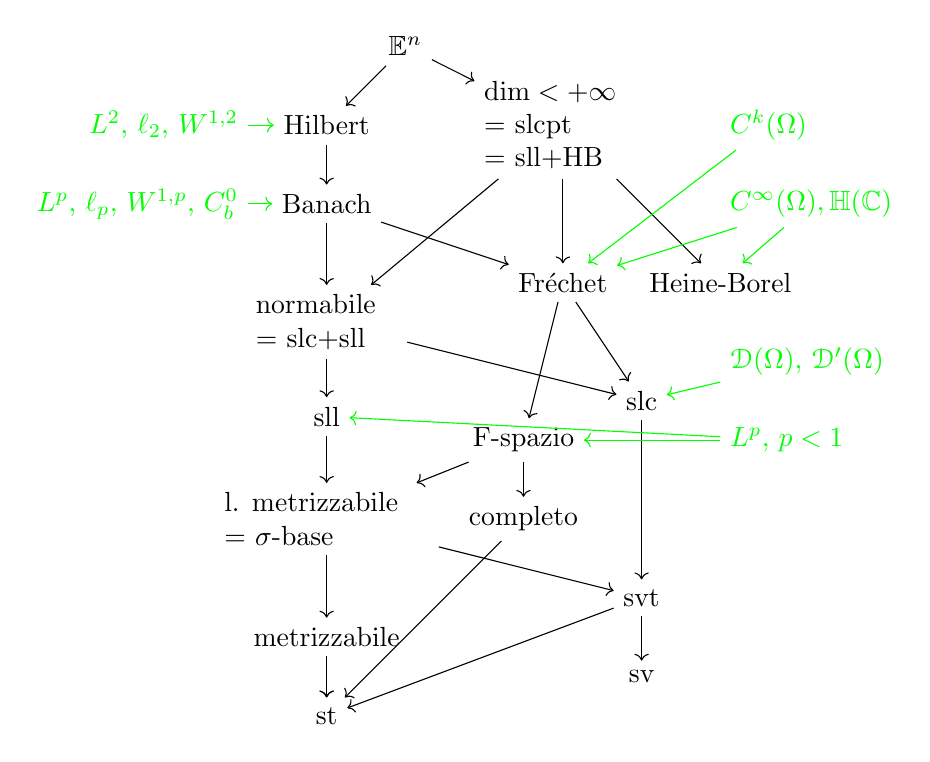
\begin{tikzpicture}[node distance=2cm]
    \draw node at (0,0)[name=En]{$\mathbb E^n$};
    \draw node at (-1,-1)[name=hilbert]{Hilbert};
    \draw node at (-1,-2)[name=banach]{Banach};
    \draw node at (-1,-3.5)[name=normabile]{\parbox[c]{1.8cm}{normabile\\= slc+sll}};
    \draw node at (-1,-4.7)[name=sll]{sll};
    \draw node at (-1,-6)[name=metrizzabile]{\parbox[c]{2.6cm}{l. metrizzabile\\= $\sigma$-base}};
    \draw node at (-1,-7.5)[name=metrico]{metrizzabile};
    \draw node at (-1,-8.5)[name=st]{st};
    \draw node at (2,-1)[name=finito,text width=2cm]{\parbox{3cm}{$\dim<+\infty$\\= slcpt\\= sll+HB}};
    \draw node at (4,-3)[name=hb]{Heine-Borel};
    \draw node at (2,-3)[name=frechet]{Fréchet};
    \draw node at (1.5,-5)[name=f]{F-spazio};
    \draw node at (3,-4.5)[name=slc]{slc};
    \draw node at (1.5,-6)[name=completo]{completo};
    \draw node at (3,-7)[name=svt]{svt};
    \draw node at (3,-8)[name=sv]{sv};

    \draw[->](En) -- (hilbert);
    \draw[->](En) -- (finito);
    \draw[->](hilbert) -- (banach);
    \draw[->](banach) -- (normabile);
    \draw[->](banach) -- (frechet);
    \draw[->](normabile) -- (sll);
    \draw[->](normabile) -- (slc);
    \draw[->](sll) -- (metrizzabile);
    \draw[->](metrizzabile) -- (metrico);
    \draw[->](metrizzabile) -- (svt);
    \draw[->](metrico) -- (st);
    \draw[->](finito) -- (hb);
    \draw[->](finito) -- (normabile);
    \draw[->](finito) -- (frechet);
    \draw[->](frechet) -- (f);
    \draw[->](frechet) -- (slc);
    \draw[->](f) -- (metrizzabile);
    \draw[->](f) -- (completo);
    \draw[->](slc) -- (svt);
    \draw[->](svt) -- (sv);
    \draw[->](svt) -- (st);
    \draw[->](completo) -- (st);
    \draw[->](metrico) -- (st);

    \begin{scope}[green]
      \draw node at (-2,-1)[name=H,left]{$L^2$, $\ell_2$, $W^{1,2}$};
      \draw[->](H) -- (hilbert);
      \draw node at (-2,-2)[name=Lp,left]{$L^p$, $\ell_p$, $W^{1,p}$, $C^0_b$};
      \draw[->](Lp) -- (banach);
      \draw node at (4,-1)[name=Ck,right]{$C^k(\Omega)$};
      \draw[->](Ck) -- (frechet);
      \draw node at (4,-2)[name=HC,right]{$C^\infty(\Omega), \HH(\CC)$};
      \draw[->](HC) -- (frechet);
      \draw[->](HC) -- (hb);
      \draw node at (4, -4)[name=D,right]{$\D(\Omega)$, $\D'(\Omega)$};
      \draw[->](D) -- (slc);
      \draw node at (4,-5)[name=Lpm,right]{$L^p$, $p<1$};
      \draw[->](Lpm) -- (f);
      \draw[->](Lpm) -- (sll);
    \end{scope}


  \end{tikzpicture}
\end{figure}

In generale un insieme $E$ in uno s.v.t.\ $V$ si dice \emph{limitato}
se è contenuto in un opportuno riscalamento di qualunque intorno dello
$0$.
Cioè $B$ è limitato se per ogni $U$ intorno di $0$ esiste $r>0$ tale
che $B\subset r U$.
\marginpar{limitato}
Osserviamo che è possibile che ogni intorno di $0$ sia illimitato, questo
ad esempio in tutti gli spazi localmente convessi non metrizzabili.
Attenzione che se anche la topologia è metrizzabile non è detto che i
limitati dello svt corrispondano ai limitati nella metrica: infatti
metriche che inducono la stessa topologia possono avere limitati
diversi (posso sempre rendere limitata una metrica mantenendo la
stessa topologia indotta).

\begin{theorem}\label{th:distanza_concava}
  Se $d$ è una distanza e $\phi\colon[0,+\infty)\to[0,+\infty)$ è una
      funzione concava con $\phi(0)=0$ allora $\phi$ è crescente e
      $d'=\phi\circ d$ è
      anch'essa una distanza che induce la stessa topologia di $d$.
\end{theorem}
\begin{proof}
  Dimostrazione omessa.
\end{proof}

Si usa tipicamente
\[
\phi(t) = \frac{t}{1+t} = 1-\frac{1}{1+t}
\]
per rendere limitata una distanza qualunque.

%% Anche il concetto di successioni di Cauchy può essere definito negli
%% spazi vettoriali topologici, anche se non sono metrizzabili. E'
%% infatti sufficiente (e necessario) avere una struttura \emph{uniforme}
%% che permetta di confrontare intorni in punti diversi dello
%% spazio. Mediante le traslazioni questo è possibile negli spazi
%% vettoriali. Tuttavia la completezza di uno spazio vettoriale
%% topologico richiede la convergenza di ogni \emph{net} di Cauchy.

%% Un net è una funzione a valori nello spazio definita su un qualunque
%% insieme diretto (un insieme con un ordine tale che dati due elementi
%% dell'insieme ce n'è sempre uno maggiore di entrambi). Se il dominio
%% del net sono i numeri naturali siamo in presenza di una usuale
%% \emph{successione}.
%% \marginpar{net}

%% Se $x_\alpha$ è un net in uno svt $X$.
%% Diremo che $x_\alpha$ converge a $x\in X$ se per ogni $U$ intorno di
%% $x$ esiste $\gamma$ tale che per ogni $\alpha\ge \gamma$ si ha
%% $x_\alpha \in U$.
%% \marginpar{convergenza di un net}
%% Diremo che $x_\alpha$ è di
%% Cauchy se per ogni $U$ intorno di $0$ esiste $\gamma$ tale che se
%% $\alpha,\beta\ge\gamma$ allora $x_\alpha -x_\beta \in U$.
%% \marginpar{net di Cauchy}

%% Uno svt $X$ si dice essere completo se ogni net di Cauchy converge.
%% \marginpar{completezza}

\section{propriet\`a di separazione}

%\cite[1.10]{Rudin}

\begin{proposition}
  Se $W$ è un intorno di $0$ in uno svt $X$ allora esiste $U$ intorno
  aperto di $0$ tale che $U=-U$ e $U+U\subset W$.
\end{proposition}

\begin{proof}
  Sfruttiamo la continuità della somma nel punto $(0,0)$. Dato un
  qualunque $W$ intorno di $0$ esistono $V_1, V_2$ intorni di $0$ tali
  che se $(x,y)\in V_1\times V_2$ allora $x+y \in W$. Questo significa
  che $V_1+V_2 \subset W$. Basterà allora prendere
  \[
  V=V_1\cap V_2,\qquad U = V \cap (-V).
  \]
\end{proof}

\begin{theorem}
  Sia $X$ uno svt, $K\subset X$ un compatto e $C\subset X$ un chiuso
  tali che $K\cap C=\emptyset$. Allora esiste un intorno $V$ di $0$
  tale che $(K+C) \cap (C+V) = \emptyset$.
\end{theorem}
\begin{proof}
  Sia $x\in K$ un punto qualunque. Visto che $x\not \in C$ e visto che
  $C$ è chiuso, esisterà un intorno aperto $W_x$ di $0$ tale che
  $(W_x + x) \cap C=\emptyset$.
  Tramite il lemma precedente possiamo considerare
  $V_x$ un intorno aperto di $0$ tale che
  $V_x+V_x +V_x \subset W_x$ e
  $V_x=-V_x$.
  Essendo $K$ compatto, ed essendo $V_x$ un
  ricoprimento aperto di $K$ al variare di $x\in K$, possiamo estrarre
  un ricoprimento finito, ovvero $x_1,\dots, x_m$ tali che
  $V_{x_i}+x_i$ ricoprono $K$ per $i=1,\dots, m$. Prendiamo quindi
  $V= V_{x_1} \cap\dots\cap V_{x_m}$ cosicchè
  $V$ è aperto.

  Per mostrare che $(K+V)\cap(C+V)=\emptyset$ è sufficiente mostrare
  che $K+V-V$ non interseca $C$.
  Sia dunque $x\in K$, $u\in V$ e $v\in V$. Esisterà $x_i$ tale che
  $x \in x_i + V_{x_i}$. Inoltre $u,v \in V \subset V_{x_i}$.
  Dunque
  \[
  x+u-v \in x_i + V_{x_i} + V_{x_i} - V_{x_i} \subset x_i +
  W_{x_i}.
  \]
  Ma, per costruzione, $x+W_x$ è disgiunto da $C$.
\end{proof}

Osserviamo che se due aperti sono disgiunti, anche la chiusura di uno
è disgiunto dall'altro.

\begin{corollary}
  Ogni svt è di Hausdorff ($T_2$).
\end{corollary}
\begin{proof}
  Dati $x,y$ in uno svt $X$ certamente $\{x\}$ è compatto e per
  ipotesi di svt abbiamo assunto che $\{y\}$ sia chiuso. Dunque
  possiamo applicare il teorema precedente per trovare un intorno
  $V$ di zero tale che $(x+V) \cap (y+V) = \emptyset$.
\end{proof}

Ricordiamo che in ogni spazio di Hausdorff gli insiemi compatti sono
anche chiusi.

\begin{corollary}
  Ogni intorno di $0$ contiene anche un intorno chiuso di $0$.
\end{corollary}
\begin{proof}
  Sia $W$ un intorno di $0$ nello svt $X$. $W$ contiene un intorno
  aperto $U$ di $0$. Sia $C=X\setminus U$ e
  $K=\{0\}$.
  Per il teorema precedente esiste $V$ intorno aperto di $0$
  tale che $V = K+V$ non interseca $C+V$. Ma allora anche
  $\overline{V}$ non interseca $C+V$ e quindi $V$ non interseca $C$.
  Dunque $\overline{V}\subset X \setminus C = U \subset W$.
\end{proof}

Un sottoinsieme $A$ di uno svt $X$ si dice essere \emph{bilanciato}
\marginpar{bilanciato}
se per ogni $x\in A$ e per ogni $c\in \CC$ si ha $cx\in A$.
L'insieme $A$ si dice \emph{convesso}
\marginpar{convesso}
se per ogni $t\in[0,a]$, $x,y\in A$ si ha $tx+(1-t)y\in A$.

\begin{theorem}
  Sia $U$ un intorno di $0$ in uno svt $X$. Allora $U$ contiene un
  intorno di $0$ bilanciato. Se inoltre $U$ è convesso allora $U$
  contiene un intorno di $0$ bilanciato e convesso.
\end{theorem}
\begin{proof}
Siccome $(\alpha, x)\mapsto \alpha x$ è continua (per definizione di svt)
e visto che $0 x= 0$, esiste un intorno $V$ di $0$ e un $\delta>0$
(intorno di $0$ in $\CC$)
tali che per ogni $\abs{\alpha} < \delta$ per ogni $x\in V$ si ha $\alpha
x\in U$ cioè $\alpha V\subset U$ per ogni $\abs{\alpha}<\delta$.
Dunque l'unione per $\abs{\alpha}< \delta$ di $\alpha V$ produce un
insieme bilanciato che contiene $V$ ed è contenuto in $U$.

Supponiamo ora che $U$ sia un intorno convesso di $0$. Poniamo
\[
W = \bigcap_{\abs{\alpha}=1} \alpha U.
\]
Siccome $W$ è intersezione di convessi, $W$ stesso è convesso.
Osserviamo inoltre che essendo $U$ convesso si ha $tU \subset U$ per
ogni $t\in [0,1]$. Dunque $tW \subset W$ per ogni $t\in[0,1]$ e,
ovviamente, $\alpha W = W$ per ogni $\abs{\alpha}=1$. Dunque per ogni
$\abs{\beta}\le 1$ si ha $\beta = t \alpha$ e $\beta W \subset
W$. Dunque $W$ è bilanciato.

Vogliamo mostrare che $W$ è un intorno di $0$. Per la continuità della
moltiplicazione $(x,t)\mapsto tx$ esiste un intorno $V$ di zero e un
$\delta>0$ tali che per ogni $\abs{\beta} < \delta$ si ha
$\beta V \subset U$. Questo significa che per ogni $\abs{\alpha}=1$
si ha $\frac{\delta}{2}\alpha^{-1} V \subset U$ ovvero
$\frac \delta 2 V \subset \alpha U$ da cui
$\frac \delta 2 V \subset W$. Ma $\frac \delta 2 V$ è un intorno di $0$ dunque
anche $W$ lo è.
\end{proof}

\begin{theorem}
  Un compatto $K$ in uno svt $X$ è limitato (oltre che chiuso, come
  già sappiamo).
\end{theorem}
\begin{proof}
  Sia $V$ un qualunque intorno di $0$. Dato $x\in K$ sappiamo che
  $x/k \to 0$ per $k\to +\infty$, cioè esiste $k\in \NN$ tale che
  $x/k \in V$. Dunque $K\subset \bigcup_{k=1}^\infty kV$.
  Estraendo un sottoricoprimento finito e osservando che $kV$ è una
  successione crescente di insiemi, deduciamo che esiste $k$ tale che
  $kV\supset K$. Dunque $K$ è limitato.
\end{proof}

\begin{theorem}\cite[1.15]{Rudin}
  Uno spazio localmente limitato (sll) ammette una base numerabile di
  intorni di $0$.
\end{theorem}
\begin{proof}
  Sia infatti $B$ un intorno limitato di $0$. $B$ contiene un intorno
  bilanciato di $0$ che a sua volta sarà limitato. Posso quindi
  supporre che $B$ sia bilanciato oltre che limitato.
  Per ogni $U$ intorno di
  $0$ esiste un $r>0$ tale che $B\subset r U$. Dunque posto  $\B = \{
  B/k\colon k\in \NN\}$ per ogni $U$ intorno di $0$ esiste un $V\in\B$
  tale che $V\subset U$ (basta prendere $k>r$ cosicché $B/k \subset r
  U /k \subset U$. Dunque $\B$ è una base di intorni di $0$.
\end{proof}

Vale anche il seguente teorema che non dimostriamo (ma si veda \cite[1.24]{Rudin}).

\begin{theorem}
  Uno svt che ammette una base numerabile di intorni di $0$ è metrizzabile.
\end{theorem}

\begin{theorem}
Se $X$ è uno svt e $Y$ è un suo sottospazio
che risulta essere un $F$-spazio (cioè metrizzabile e completo) allora
$Y$ è chiuso in $X$.
\end{theorem}
\begin{proof}
  Sia $d$ una metrica invariante su $Y$ e definiamo
  $B_k=\{ y\in Y\colon d(y,0) < 1/k\}$. Visto che i $B_k$ sono aperti
  in $Y$ devono esistere $U_k$ aperti in $X$ tali che
  $B_k=Y\cap U_k$. Gli $U_k$ sono intorni di $0$ in $X$.

  Consideriamo un punto $x\in \bar Y$. Per definizione ogni
  $Y\cap x+U_k$ è non vuoto.
  Dunque esiste $x_k \in Y\cap (x+U_k)$. Chiaramente $x_k$ è di Cauchy
  in $Y$ in quanto dato un qualunque intorno $U$ di $0$ esiste $m$
  tale che
  $U_m-U_m\subset U$ e quindi per ogni $k,j\ge m$ si ha $x_j-x \in
  U_m$, $x_k-x \in U_m$ da cui $x_k-x_j\in U_m -U_m \subset U$.
  Dunque $x_k$ converge in $Y$ ma non può che convergere a $x$, dunque
  $x\in Y$. Da cui $Y=\bar Y$.
\end{proof}

\section{Spazi localmente convessi e seminorme}

Uno svt X si dice essere uno slc (spazio localmente convesso) se
esiste una base di intorni convessi di $0$.

Un insieme $A$ si dice \emph{assorbente} se per ogni $x\in X$ esiste
$r>0$ tale che $x\in rA$.
Ovviamente se $X$ è uno svt
ogni intorno $U$ di $0$ è assorbente
in quanto per ogni $x\in X$, si ha $x/r\to 0$ per $r\to +\infty$ e
quindi per ogni $r$ sufficientemente grande si ha $x/r \in U$ ovvero
$x \in rU$.

\begin{theorem}\label{th:slc_base}
  Sia $X$ uno spazio vettoriale e sia $\F$ una famiglia non vuota di
  sottoinsiemi di $X$ tali che ogni $B\in \F$ sia: convesso,
  bilanciato e assorbente. Supponiamo inoltre che $\F$ sia
  \emph{separante} cioè che per ogni $x\neq 0$ esista $B\in \F$ ed
  esista $r>0$ tale che $rx \not \in B$.

  Allora se consideriamo $\B$ la famiglia di tutte le intersezioni
  finite di riscalati di elementi di $\F$:
  \[
    \B \defeq \{ \bigcup_{k=1}^N r_k B_k \colon r_k>0, B_k\in \F\}
  \]
  $\B$ risulta essere la base di intorni
  di $0$ di una topologia invariante $\tau$ che rende $X$ uno slc.
\end{theorem}
%
\begin{proof}
  Si definisce:
  \[
  \tau = \{ A \subset X \colon \forall x \in A\, \exists B \in \B
  \colon x \in x+ B \subset A\}.
  \]

  Verifichiamo che $\tau$ è una topologia. Unione di elementi di
  $\tau$ è ovviamente elemento di $\tau$ (qualunque sia $\B$).
  $X \in \tau$ in quanto $\B$ è non vuota e per ogni $B\in \B$ si ha $0\in B$
  essendo $B$ bilanciato.
  Per garantire che l'intersezione di due elementi di $\tau$ sia
  elemento di $\tau$ è sufficiente che intersezione di elementi di
  $\B$ contenga un elemento di $\B$. Ma questo è vero perché, per come
  è stata definita $\B$, l'intersezione di due elementi di $\B$ è ancora
  elemento di $\B$.
  Dunque $\tau$ è una topologia invariante per traslazioni di cui $\B$
  è una base di intorni di $0$.

  Affinché $(X,\tau)$ sia uno spazio vettoriale topologico dobbiamo
  mostrare che somma e prodotto sono operazioni continue e che $\{0\}$
  è chiuso. Una volta mostrato che $X$ è uno svt è ovvio che $X$ sia
  uno slc in quanto $\B$ è per costruzione una base di intorni
  convessi di $0$.

  Innanzitutto osserviamo che gli elementi di $\B$ sono anch'essi
  insiemi convessi, bilanciati e assorbenti. Infatti intersezione di
  bilanciati è bilanciato, intersezione di convessi è convesso,
  intersezione di bilanciati assorbenti è assorbente.

  Per dimostrare che la somma è continua è sufficiente dimostrare che
  per ogni $U$ intorno di $0$ esiste $V$ intorno di zero tale che
  $V+V\subset U$. Ma questo è facile da ottenere in quanto gli insiemi
  convessi bilanciati $B$ soddisfano la proprietà $B = B/2 + B/2$.

  Per dimostrare la continuità del prodotto $(\alpha,x)\mapsto \alpha
  x$ dobbiamo lavorare un pochino di più. Cerchiamo di mostrare che il
  prodotto è continuo nel punto $(\alpha_0, x_0)$ in $\CC \times X$.
  Dato $U$ un intorno di $0$ vogliamo mostrare che esiste un $W$
  intorno di $0$ e un $\eps>0$ tali che per ogni $\abs{\alpha}<\eps$ e
  per ogni $x\in W$ si ha $\alpha x- \alpha x_0 \in U$.

  Prendiamo $V$ un intorno convesso, bilanciato, assorbente di $0$
  tale che $V+V \subset U$ (questo è
  possibile per quanto osservato prima).
  Essendo $V$ assorbente esisterà $r>0$ tale che $x_0\in r V$.
  Scegliamo allora $\eps = 1/r$ e $W=V/(\abs{\alpha_0}+\eps)$.
  Si avrà allora per ogni $\abs{\alpha-\alpha_0}<\eps$ e per ogni
  $x\in x_0 + W$:
  \begin{align*}
    \alpha x - \alpha_0 x_0
    &= \alpha(x-x_0) + (\alpha -\alpha_0) x_0
    \in \alpha W + (\alpha-\alpha_0) r V \\
    &\subset \abs{\alpha} W + \abs{\alpha-\alpha_0} r V
    \subset (\abs{\alpha_0} + \eps) W + \eps r V\\
    &= V + V \subset U.
  \end{align*}
  Dunque anche la moltiplicazione è continua.

  Ci resta da dimostrare che $\{0\}$ è chiuso. Dimostriamo che ogni
  $x\neq 0$ ha un intorno aperto disgiunto da $0$. Dato $x\neq 0$ per
  l'ipotesi di separazione di $\F$ sappiamo che esiste
  $B\in \F\subset \B$ tale che $x \not \in B/r$ per qualche
  $r>0$. Dunque $0 = x- x \not \in x- B/r$. Ma $-B/r = B/r$ è un
  intorno di $0$ e quindi $x$ è punto interno al complementare di $\{0\}$.

\end{proof}

Una funzione $p\colon V \to \RR$ si dice seminorma se soddisfa le
seguenti proprietà:
\marginpar{seminorma}
\begin{enumerate}
\item $p(v+w)\le p(v) + p(w)$ (subadditività)
\item $p(\alpha v) = \abs{\alpha} p(v)$ ($1$-omogeneità)
\end{enumerate}
Diremo che una seminorma $p$ è una \emph{norma} se inoltre verifica la
proprietà
\begin{enumerate}
  \item[3.] $p(v)=0 \Rightarrow v=0$.
\end{enumerate}

\begin{theorem}
  Le seminorme hanno le seguenti proprietà:
  \begin{enumerate}
  \item $p(0)=0$;
  \item $\abs{p(x)-p(y)} \le p(x-y)$;
  \item $p(x)\ge 0$;
  \item $\{p(x) = 0\}$ è un sottospazio vettoriale di $X$;
  \item $B_p=\{x\in X\colon p(x)<1\} $ è bilanciato, convesso, assorbente.
  \end{enumerate}
\end{theorem}

\begin{proof}
  Si ha  $p(0) = p(0\cdot 0) = \abs{0}p(0) = 0p(0) = 0$.
  Inoltre dalla subadditività:
  \[
  p(x) = p(x-y+y) \le p(x-y) + p(y)
  \]
  si ottiene $p(x) - p(y) \le p(x-y) = p(-1(y-x)) = p(y-x)$.
  Scambiando $x$ con $y$ si ottiene dunque la disuguaglianza cercata.
  Ponendo poi $y=0$ si ottiene $p(x) \ge \abs{p(x)}\ge 0$.
  Presi $x,y\in \{p=0\}$ si ha $p(x+y) \le p(x) + p(y) = 0 + 0 = 0$
  dunque $x+y\in \{p=0\}$. Inoltre $p(\alpha x)=\abs{\alpha} p(x)=0$
  da cui anche $\alpha x \in \{p=0\}$.

  Chiaramente $B_p$ è bilanciato per
  omogeneità di $p$. Dati $x,y \in B_p$ e $t\in[0,1]$ si ha
  \begin{align*}
    p(tx+ (1-t)y) &\le p(tx) + p((1-t)y) \\
    &= tp(x) + (1-t)p(y) \le t + (1-t)
    = 1
  \end{align*}
  dunque $B_p$ è convesso.
  Per mostrare che $B_p$ è assorbente si
  prende un qualunque $x\in X$ e si sceglie $t > p(x)$. Allora
  $p(x/t) = p(x)/t < 1$ da cui $x\in t B_p$.
\end{proof}

\begin{theorem}
  Sia $p$ una seminorma su uno svt $X$. Sono equivalenti:
  \begin{enumerate}
  \item $p$ è continua;
  \item $p$ è continua in $0$;
  \item $B_p=\{p<1\}$ è aperto.
  \end{enumerate}
\end{theorem}
\begin{proof}
  Ovviamente 1 implica 2 e 2 implica 3. Dimostriamo che 3 implica
  1. Sia dunque $p$ una seminorma tale che $B_p=\{ p<1 \}$ è aperto.
  Dato un punto $x\in X$ vogliamo dimostrare che $p$ è continua in
  $x$.
  Per ogni $\eps>0$ dobbiamo quindi determinare un intorno $U$ di $x$ tale che
  $p(U) \subset (p(x)-\eps, p(x)+\eps)$.
  Scegliamo $U = x + \eps B_p$. Dato $y\in x + U$ si ha
  $y= x + \eps u$
  con $u\in B_p$ cioè $p(u)< 1$. Ma da un lato si ha
  \[
  p(x+\eps u) \le p(x) + \eps p(u) < p(x) + \eps
  \]
  e dall'altro
  \[
  p(x+\eps u) \ge p(x) - \eps p(u) > p(x) - \eps
  \]
  e il teorema è dimostrato.
\end{proof}

Una famiglia $\P$ si seminorme su uno svt $X$ si dice \emph{separante}
\marginpar{separante}
se per ogni $x\neq 0$ esiste $p\in \P$ tale che $p(x)>0$.

\begin{theorem}
Sia $\P$ una famiglia di seminorme separanti definite su uno spazio vettoriale
$X$. La topologia $\tau$ generata dalla base di intorni di $0$
data dalle intersezioni finite degli insiemi
\[
 r B_p = \{x\in X \colon p(x) < r\}
\]
al variare di $r>0$ e $p\in \P$, rende $X$ uno slc (spazio vettoriale
localmente convesso). Inoltre $\tau$ è
caratterizzata come la più debole topologia che rende $X$ uno svt
e che rende continua ogni
seminorma $p\in \P$.

A posteriori osserviamo che è sufficiente prendere $r=1/n$. Dunque se
$\P$ è numerabile si può trovare una base numerabile di intorni di $0$.
\end{theorem}
\begin{proof}
  Consideriamo la famiglia $\F=\{ r B_p \colon r>0, p\in \P\}$. Questa
  è una famiglia di insiemi convessi, bilanciati, assorbenti.
  Il fatto che $\P$ sia separante significa che anche $\F$ è
  separante.

  Per un teorema precedente sappiamo quindi
  che $\F$ genera una topologia $\tau$ che rende $X$ uno
  slc.

  Chiaramente la topologia $\tau$ rende continue tutte le seminorme
  $p\in \P$ in quanto $B_p$ è aperto per costruzione
  e si può applicare il teorema precedente.

  Inoltre ogni topologia invariante per traslazioni
  che rende continue tutte le seminorme
  $p\in \P$ deve contenere almeno le $B_p$ come intorni di $0$ e di
  conseguenza deve contenere ogni $r B_p$ e ogni intersezione finita
  di questi.
\end{proof}

Dato un insieme $B$ assorbente possiamo definire
un funzionale (detto \emph{gauge} o funzionale di Minkowski):
\[
\mu_B(x) = \inf \{t>0 \colon x/t \in B \}.
\]

\begin{theorem}
  Se $p$ è una seminorma
  si ha $p=\mu_{B_p}$.
\end{theorem}

\begin{proof}
  Osserviamo che:
  \begin{align*}
    \mu_{B_p}(x)
    &= \inf \{t > 0\colon p(x/t) < 1\}
    = \inf \{t>0\colon p(x) < t\} \\
    & = \inf (p(x),+\infty) = p(x).
  \end{align*}
\end{proof}

\begin{theorem}
Sia $B$ bilanciato, convesso, assorbente, in uno spazio vettoriale
$X$.
Risulta che $\mu_B$ è una seminorma su $X$. Inoltre
\[
\{\mu_B < 1\} \subset   B\subset \{\mu_B \le 1\}.
\]
\end{theorem}
\begin{proof}
Chiaramente $\mu_B$ è finito (in quanto $B$ è assorbente) ed è omogeneo
(per definizione).
Mostriamo la subadditività.
Siano $t=\mu_B(x)+\eps$, $s=\mu_B(y)+\eps$ per qualche $\eps>0$.
Allora $x/t, y/t\in B$ e siccome $B$ è convesso anche la loro combinazione:
\[
\frac{x+y}{s+t} = \frac{t}{s+t} \frac{x}{t} + \frac{s}{s+t}\frac{y}{s}.
\]
Dunque, per ogni $\eps>0$,
\[
\mu_B(x+y) = (s+t)\mu_B\left(\frac{x+y}{s+y}\right) \le s+t = \mu_B(x)
+ \mu_B(y) + 2\eps
\]
e la subadditività è dimostrata.

Chiaramente se $\mu_B(x)<1$ si ha $x \in B$ e se $\mu_B(x)>1$ si ha
$x\not \in B$ (basta osservare che essendo $B$ assorbente e convesso,
fissato $x$
l'insieme $\{t>0 \colon x/t\in B\}$ è un intervallo illimitato e
quindi coincide con uno dei
seguenti: $[\mu_B(x),+\infty)$ o $(\mu_B(x),+\infty)$.
\end{proof}

\begin{theorem}
  Sia $X$ uno slc. Allora la topologia di $X$ è generata da una famiglia
  di seminorme.
\end{theorem}
\begin{proof}
  Sia $\B$ una base di intorni convessi di $0$. Possiamo supporre che ogni
  $B\in \B$ sia aperto (la parte interna di un convesso è convessa).
  E' chiaro allora che la famiglia di seminorme
  $\P=\{\mu_B \colon B\in \B\}$ genera la topologia di $X$.
\end{proof}

\begin{theorem}\label{th:slc_conv}
  Sia $X$ uno slc la cui topologia è generata da una famiglia di
  seminorme $\P$.
  Allora si ha $x_j\to x$ se e solo se per ogni
  $p\in \P$ si ha $p(x_j-x)\to 0$.
\end{theorem}
%
\begin{proof}
  Chiaramente se $x_j \to x$ si ha $p(x_j-x)\to 0$ in quanto le
  seminorme $p_j$ sono continue.

  Viceversa supponiamo che $p(x_j-x)\to 0$ per ogni
  $p\in \P$. Dato un intorno $U$ di $0$ vogliamo mostrare che $x_j-x$
  sta definitivamente in $U$.
  L'intorno $U$ deve contenere una intersezione finita di riscalamenti
  di palle unitarie delle seminorme:
  \[
  U \supset \bigcap_{k=1}^m r_k B_{p_k}.
  \]
  Ma per ogni $k$ si ha $p_k(x_j-x)\to 0$ quindi esiste $N_k$ tale che
  per ogni $j>N_k$ si ha $p_k(x_j-x) < r_k$. Questo significa che per
  tali indici $j$ si ha $x_j-x \in r_k B_{p_k}$. Posto $N=\max_{k=1}^m
  N_k$ si ha il risultato voluto.
\end{proof}

\begin{theorem}\label{th:slc_metrizzabile}
  Se $\P$ è una famiglia separante, numerabile di seminorme sullo spazio
  vettoriale $X$ allora la topologia $\tau$ generata da $\P$
  è metrizzabile.
\end{theorem}
%
\begin{proof}
  Sia $\P=\{p_k\}_{k\in\NN}$ e definiamo
  \[
  d(x,y) = \max_k \frac{1}{2^k}\frac{p_k(x-y)}{1+p_k(x-y)}.
  \]
  Chiaro che $d$ soddisfa la disuguaglianza triangolare in quanto è
  massimo
  di distanze (si
  veda il Teorema~\ref{th:distanza_concava}). Inoltre $d(x,y)=0$
  implica $x=y$ in quanto $\P$ è separante.
  E' anche ovvio che la distanza è invariante per traslazioni. Dunque
  è sufficiente dimostrare che le palle $B_r = \{x\colon d(x,y)<r\}$
  formano una base di intorni per la topologia $\tau$.

  Da un lato osserviamo che $d(x)<r$ equivale a
  \[
  (2^{-k}-r) p_k(x) < r
  \]
  che è certamente soddisfatta per tutti i $k>\log_2(1/r)$,
  mentre per i rimanenti (finiti) indici $k$ si deve avere
  \[
  p_k(x) < \frac{r}{2^{-k}-r} =: r_k
  \]
  dunque $B_r$ risulta essere uguale ad una intersezione finita di
  insiemi della forma $r_k B_{p_k}$ e dunque contiene un intorno di
  $0$ della topologia $\tau$.

  Viceversa dato un qualunque intorno $W$ di $0$ per $\tau$ questo
  contiene una intersezione finita $k=1,\dots,m$ di insiemi della forma
  $r_k  B_{p_k}$.
  Basterà scegliere $r>0$ in modo che
  \[
  2r < \min_{k=1}^m 2^{-k} r_k
  \]
  infatti in tal caso ogni $x\in B_r$ soddisfa
  \[
  \frac{1}{2^k} \frac{p_k(x)}{1+p_k(x)} < r < \frac{2^{-k}r_k}{2}
  \]
  da cui segue $p_k(x) < r_k$. Dunque $B_r\subset W$.
\end{proof}

\begin{theorem}
  Sia $X$ uno slc generato da una famiglia di seminorme $\P$.
  Un insieme $C\subset X$ è limitato se e solo se ogni seminorma
  $p\in\P$ è
  limitata su $C$.
\end{theorem}
%
\begin{proof}
  Se $C$ è limitato allora per ogni $U$ intorno di $0$ esiste $r>0$
  tale che $C\subset rU$. In particolare preso $U=B_p$ si ha
  $C\subset rB_p$ che significa che $p(x)<r$ per ogni $x\in C$.

  Viceversa supponiamo che ogni $p\in\P$ sia limitata su $C$. Dato un
  qualunque $U$ intorno di $0$ sappiamo che $U$ contiene un intorno
  del tipo
  \[
  U \supset \bigcap_{k=1}^m r_k B_{p_k},\qquad p_k\in\P.
  \]
  Sappiamo che per ogni $k$ esiste $c_k$ tale che $p_k(x)<c_k$ per
  ogni $x\in C$. Posto
  \[
   r \defeq \max_{k=1}^m \frac{c_k}{r_k}
   \]
   si trova che ogni $x\in C$ sta in $r r_k B_{p_k}$ e quindi sta in
   $t U$.
\end{proof}


\begin{theorem}
  Uno svt $X$ è normabile se e solo se esiste un intorno convesso e
  limitato di $0$.
\end{theorem}
\begin{proof}
  Se $X$ è normabile è chiaro che la palla unitaria della norma è un
  convesso limitato (ogni intorno di $0$ contiene un riscalamento
  della palla per definizione).

  Viceversa sia $B$ un intorno convesso, limitato di $0$. Siccome $B$
  è un intorno di $0$ deve essere assorbente (in quanto per ogni $x$
  si deve avere $x/k\to 0$ per la continuità del prodotto e dunque $x$
  deve stare in $k B$). Dunque $p(x)=\mu_B(x)$ risulta essere una
  seminorma su $X$.

  Mostriamo ora che $p$ è una norma. Supponiamo che
  ci sia $x\neq 0$ tale che $p(x)=0$. Siccome $\{0\}$ è chiuso esiste
  un intorno $U$ di $0$ tale che $x\not \in U$. Ma allora non esiste
  $r>0$ tale che $B\subset rU$ in quanto per ogni $r>0$ si ha
  $p(rx)=rp(x)=0$ dunque $rx\in B$ ma $rx\not \in rU$.

  Mostriamo ora che la topologia generata da $\P=\{p\}$ coincide con
  $\tau$ la topologia originale su $X$. Visto che $B_p=B$ è un intorno
  di zero per $\tau$, è chiaro che la topologia indotta da $p$ è meno
  fine di $\tau$. Viceversa dato un intorno $U$ di zero per $\tau$
  siccome $B$ è limitato esiste $r>0$ tale che $B_p=B\subset rU$ cioè
  $B_p/r \subset U$ e dunque la topologia indotta da $p$ è più fine di
  $\tau$.
  \end{proof}

\section{lo spazio delle funzioni continue}

Sia $C(\Omega)$ lo spazio vettoriale delle funzioni continue definite
\marginpar{$C(\Omega)$}
su $\Omega$ aperto di $\RR^n$ a valori in $\CC$ (o in
$\RR$).
Su $C(\Omega)$ possiamo mettere la topologia generata dalle
seminorme
\[
p_K(f) \defeq \max_{x\in K} \abs{f(x)}
\]
dove $K$ è un qualunque compatto in $\Omega$.
Osserviamo subito che se scegliamo una famiglia crescente di compatti
$K_j$ che invade $\Omega$ allora ogni compatto $K$ risulta incluso in uno dei
$K_j$ e quindi le seminorme $p_{K_j}$ generano la stessa topologia
generata da tutte le $p_K$.

Inoltre se $K_j$ è crescente,
l'intersezione finita di riscalati dei convessi $B_{p_{K_j}}$
contiene un riscalato della $B_{p_{K_N}}$ con $N$ il massimo degli
indici considerati, dunque una base della topologia è data dalle
singole palle $B_{p_{K_j}}$ senza necessità di farne l'intersezione
finita.

Essendo le $p_{K_j}$ una quantità numerabile
risulta inoltre che questo spazio è metrizzabile.
La convergenza è data quindi dalla convergenza uniforme su ogni
compatto e determina la topologia dello spazio.
Lo spazio è anche
completo, perché se $f_k$ è una successione di Cauchy, allora su ogni
$K$ la successione $f_k$ converge ad una funzione continua $f$ che
quindi risulta essere definita su tutto $\Omega$. La convergenza
uniforme su ogni compatto implica inoltre la convergenza in $C(\Omega)$ e
dunque abbiamo mostrato che ogni successione di Cauchy converge.

Risulta quindi che $C(\Omega)$ è uno spazio di Frechét.

\section{Spazi di funzioni regolari}

Chiamiamo \emph{multi-indice} un elemento
\marginpar{multi-indici}
$\alpha = (\alpha_1, \dots, \alpha_n) \in \NN^n$
(intendiamo qui che $0\in \NN$).
Per ogni $x\in \RR^n$ e $\alpha\in \NN^n$ possiamo definire $x^\alpha
\in \RR$ tramite
\[
  x^\alpha \defeq x_1^{\alpha_1}\cdots x_n^{\alpha_n}.
\]
Analogamente possiamo definire l'operatore differenziale
\[
D^\alpha \defeq \left(\frac{\partial}{\partial x_1}\right)^{\alpha_1}\!\!\cdots
\left(\frac{\partial}{\partial x_n}\right)^{\alpha_n}\!\!.
\]
L'ordine di $D^\alpha$ (ovvero il numero di derivate)
è la \emph{lunghezza} di $\alpha$:
\[
\abs{\alpha} \defeq \alpha_1 + \dots + \alpha_n.
\]

Lo spazio $\E(\Omega)\defeq C^\infty(\Omega)$ è lo spazio delle funzioni scalari
\marginpar{$\E(\Omega)$}
definite su $\Omega$ che ammettono derivate di ogni ordine. Su tale
spazio, $D^\alpha\colon \E(\Omega)\to \E(\Omega)$ è definito per ogni $\alpha$.

Se $\Omega\subset \RR^n$, per ogni $\alpha \in \NN^n$ e per ogni
compatto $K$ di $\Omega$ possiamo definire una seminorma:
\begin{equation}\label{eq:palphaK}
p_{\alpha,K}(f) \defeq \max_{x\in K} \abs{D^\alpha f(x)}.
\end{equation}
Chiaramente queste seminorme separano $\E(\Omega)$ in quanto
per ogni $x\in \Omega$ posto $K=\{x\}$ e $\alpha=0$ si ha $\abs{f(x)}=0$.
Dunque $\E(\Omega)$ risulta essere uno spazio
localmente convesso con la topologia generata da suddette
seminorme. Inoltre selezionando una successione di compatti $K_j$ che
invade $\Omega$ è chiaro che le seminorme $p_{\alpha,K_j}$ generano la
stessa topologia in quanto se $K_j \supset K$ allora $p_{\alpha,K}\ge
p_{\alpha, K_j}$ e quindi $B_{p_{\alpha,K}}\subset B_{p_{\alpha, K_j}}$.
Visto che quest'ultima famiglia di seminorme è numerabile la topologia
generata risulta essere metrizzabile.
La convergenza è data dalla convergenza
uniforme di tutte le derivate su ogni compatto.

Inoltre lo spazio risultante è completo in quanto data una successione
di Cauchy $f_k$ la successione e tutte le sue derivate convergono
uniformemente su ogni compatto $K$ ad una funzione $f$ definita su
tutto $\Omega$. Dunque $\E(\Omega)$ risulta essere uno spazio di
Frechét.

Inoltre $\E(\Omega)$ ha la proprietà di Heine-Borel. Infatti
data una qualunque successione $f_k$ in un insieme limitato $C$ di
$\E(\Omega)$,
per la
caratterizzazione dei limitati sappiamo che ogni seminorma $p_j$
risulta limitata su tale successione e quindi la successione e tutte
le sue derivate sono uniformemente limitate su ogni compatto $K$. Per
Ascoli-Arzelà la successione ammette una estratta convergente.

$\E(\Omega)$ non è localmente limitato, altrimenti sarebbe
localmente compatto e avrebbe dunque dimensione finita, cosa che non
è, ma la vedremo tra poco.
Dunque
$\E(\Omega)$ non è normabile.

Definiamo il supporto di una funzione $f$ come il più piccolo chiuso
al di fuori del quale la funzione si annulla:
\[
\spt f \defeq \overline{\{x\in \Omega\colon f(x)\neq 0\}}.
\]

Fissato un compatto $K\subset \Omega$ possiamo definire
\[
\D_K(\Omega) \defeq \{ f\in \E(\Omega)\colon \spt f \subset K\}.
\]
Su $\D_K(\Omega)$ consideriamo la topologia indotta da
$\E(\Omega)$ cosicché $\D_K(\Omega)$ risulta essere un
sottospazio vettoriale di $\E(\Omega)$. Visto che la
convergenza di $\E(\Omega)$ è più forte della convergenza
uniforme su $K$ (data da $p_{0,K}$) se $f_k\in \D_K(\Omega)$ e
$f_k\to f$ si trova che il
supporto di $f$ è anch'esso contenuto in $K$, dunque
$f\in \D_K(\Omega)$.
Dunque $\D_K(\Omega)$ è un sottospazio vettoriale
chiuso di $\E(\Omega)$. La topologia di $\D_K(\Omega)$ è
generata dalle seminorme $p_{\alpha,K}$ in quanto se $J$ è un altro
compatto di $\Omega$ si ha $p_{\alpha,K}(f)\ge p_{\alpha,J}(f)$ per
ogni $f\in \D_K(\Omega)$.

In effetti possiamo osservare che la topologia di $\D_K(\Omega)$ non
dipende da $\Omega$... qualunque aperto contenente $K$ determina lo
stesso spazio con la stessa topologia (ogni funzione di $\D_K(\Omega)$
può essere estesa a zero fuori da $\Omega$ per determinare una
funzione in $\D_K(\RR^n)$, e viceversa la funzione in $\D_K(\RR^n)$
può essere ristretta ad $\Omega$). Dunque scriveremo più semplicemente
$\D_K$ al posto di $\D_K(\Omega)$.

E' utile osservare che $\D_K$ ha dimensione infinita se $K$ ha parte
interna non vuota. Se $K$ contiene una palla, conterrà anche una
quantità numerabile di palle di raggio sempre più piccolo. Su ognuna
di queste palle possiamo trovare una funzione non nulla a supporto
compatto nella palla, utilizzando il teorema seguente.
Chiaramente queste funzioni sono tra loro
indipendenti. Dunque $\D_K$ ha dimensione infinita (se $K$ ha parte
interna non vuota) e di conseguenza $\E(\Omega)$ ha dimensione
infinita (se $\Omega$ non è vuoto!)

\begin{theorem}\label{th:fun_cpt}
  \begin{enumerate}
    \item
      Esiste una funzione $f\in \E(\RR)$ tale che $0\le f(x)< 1$
      per ogni $x \in \RR$,
      $f(x) = 0$ se $x\le 0$ e $f(x) > 0$ se $x>0$;
    \item
      esiste una funzione $g\in \E(\RR)$ tale che $0\le g(x)
      \le 1$ per ogni $x\in \RR$, $f(x)=0$ per $x\le 0$ e $f(x)=1$ per
      $x\ge 1$.
    \item
      Dati $0<r<R$ esiste una funzione $\phi\in \E(\RR^n)$ tale
      che $\phi(x) = 1$ per $\abs{x}\le r$, $\phi(x)=0$ per
      $\abs{x}\ge R$ e $\abs{x} \in [0,1]$ per ogni $x\in \RR^n$.
  \end{enumerate}
\end{theorem}
%
\begin{proof}
  La funzione $f\colon \RR \to \RR$ può essere definita come segue
  \[
  f(x) =
  \begin{cases}
    e^{-\frac{1}{x}}& \text{per $x>0$}\\
    0 & \text{per $x\le 0$}.
  \end{cases}
  \]
  Con un poco di attenzione si può verificare che tutte le derivate di
  questa funzione risultano continue e si annullano per $x=0$ in
  quanto l'esponenziale $e^{-1/x}$ tende a zero per $x\to 0$, più
  velocemente di qualunque potenza di $x$.

  La funzione $g$ può essere definita tramite $f$:
  \[
  g(x) = \frac{f(x)}{f(x) + f(1-x)}.
  \]
  Il denominatore non si annulla mai, dunque la funzione è in
  $C^\infty$. Inoltre le proprietà richieste discendono facilmente
  dalle proprietà di $f$.

  La funzione $\phi$ si definisce quindi come
  \[
  \phi(x) = g\left(\frac{R-x}{R-r}\right).
  \]
\end{proof}

\section{lo spazio delle funzioni test}

Definiamo $\D(\Omega) \defeq C_c^\infty(\Omega)$ con $\Omega$ aperto non
\marginpar{$\D(\Omega)$}
vuoto di $\RR^n$ come lo spazio delle funzioni $f\in \E(\Omega)$
il cui supporto $\spt f$ è compatto in $\Omega$.

La funzione $\phi\in\D(\Omega)$ viene chiamata
\emph{funzione test}.
\marginpar{funzioni test}
Chiaramente $\D(\Omega)$ è uno spazio vettoriale
(complesso se le funzioni sono a valori in $\CC$).


Vogliamo mettere una topologia su $\D(\Omega)$.
Osserviamo che si ha
\[
\D(\Omega)=\bigcup_{\text{$K$ compatto in $\Omega$}} \D_K.
\]
Si tratterà dunque di ``fare il
limite per $K\to \Omega$'' delle topologie sui $\D_K$.

\emph{Osservazione.} Si potrebbe mettere su $\D(\Omega)$ la topologia
indotta da $\E(\Omega)$, ma tale topologia non sarebbe
sufficientemente forte. Infatti $\D(\Omega)$ non risulterebbe neanche
chiuso (e quindi non completo). Per fare un esempio è sufficiente
prendere un successione $\phi_k \in \D(\RR^n)$ di funzioni che valgono
$1$ su $B_k(0)$ e che valgono $0$ su $B_{k+1}(0)$ (l'esistenza di tali
funzioni è garantita dal teorema~\ref{th:fun_cpt}).
Tale successione converge uniformemente su ogni compatto (in quanto è
definitivamente costante $1$ su ogni compatto) e quindi
converge in $\E(\RR^n)$ alla funzione $1$.
Tale successione è in $\D(\Omega)$ ma il limite no.

\begin{theorem}
  Sullo spazio vettoriale $\D(\Omega)$ è definita
  la più fine topologia $\tau$ di slc che rende le immersioni
  $\D_K  \hookrightarrow \D(\Omega)$ continue per ogni compatto
  $K\subset \Omega$.

  Risulta inoltre che la topologia indotta da $\D(\Omega)$ su $\D_K$
  coincide con la topologia già definita su $\D_K$.
\end{theorem}
%
\begin{proof}
  Sia $\tau_K$ la topologia di $\D_K$ con $K$ compatto in $\Omega$.
  Affinché ogni immersione
  $i_K\colon \D_K \to \D(\Omega)$
  sia continua è necessario che l'intersezione di ogni aperto di
  $\D(\Omega)$ con $\D_K$ sia in $\tau_K$. D'altra parte perché la
  topologia sia localmente convessa deve essere determinata da una
  base di intorni aperti, convessi bilanciati di $0$.

  Definiamo dunque $\B$
  come la famiglia di tutti gli insiemi
  convessi e bilanciati in $\D(\Omega)$ tali che la loro intersezione
  con $\D_K$ sia elemento di $\tau_K$. Tali insiemi $B$ sono
  automaticamente assorbenti in quanto ogni $f\in \D(\Omega)$ sta in
  un qualche $\D_K$ e l'intersezione $B\cap \D_K$ essendo un intorno
  di $0$ in $\D_K$ è necessariamente assorbente in $\D_K$.

  Dunque per il Teorema~\ref{th:slc_base} sappiamo che $\B$ è la base di una
  topologia slc su $\D(\Omega)$.

  Inoltre tale topologia chiaramente
  rende continua ogni immersione
  $i_K\colon \D_K \hookrightarrow \D(\Omega)$.
  E' anche la più fine topologia con tale proprietà. Infatti una
  topologia localmente convessa è univocamente determinata dagli
  intorni convessi, bilanciati e aperti di $0$ e noi abbiamo
  dichiarato come aperti il massimo possibile di insiemi bilanciati e
  convessi in modo da mantenere la continuità delle immersioni.

  Chiaro dunque che se $A$ è un aperto in $\D(\Omega)$ allora per ogni
  compatto $K$ si ha che $A\cap \D_K=i_K^{-1}(A)$
  è aperto in $\D_K$.

  Viceversa vogliamo dimostrare che ogni aperto $A$ in $\D_K$ è
  intersezione di un aperto $A'$ di $\D(\Omega)$ con $\D_K$.
  Ricordiamoci che la topologia su $\D_K$ è generata dalle seminorme
  $p_\alpha = p_{\alpha,K}$ definite in \eqref{eq:palphaK}. Se
  $A=\{f\in \D_K\colon p_\alpha(f)< r\}$ per qualche $\alpha\in\NN^n$
  e $r>0$, allora si ha chiaramente $A=A'\cap \D_K$ con
  $A'=\{f\in  \D(\Omega)\colon p_\alpha(f)< r\}$.
  Lo stesso rimane vero se $A$ è intersezione finita di insiemi di
  quella forma, ovvero se $A$ è un elemento della base di $\D_K$
  definita dalle seminorme $p_\alpha$. Ma ogni aperto $A$ è unione di
  traslati di elementi di questo tipo. Il risultato segue.

\end{proof}

La costruzione che abbiamo appena fatto è quella di limite
induttivo.
La topologia risultante si chiama \emph{topologia finale}.

%%
\begin{theorem}
  \begin{enumerate}
  \item Per ogni $\alpha\in \NN^n$, la seminorma su $\D(\Omega)$
    definita da
    \[
    p_\alpha(f)\defeq \max_{x\in \Omega} \abs{D^\alpha(f)}
    \]
    è continua.

  \item Un insieme $E\subset \D(\Omega)$ è limitato se e solo se esiste
    un compatto $K\subset \Omega$ per cui $E\subset \D_K$ e inoltre
    per ogni $\alpha\in\NN^n$
    \[
    \sup_{f\in E} \max_{x\in K} \abs{D^\alpha f(x)} < +\infty.
    \]

  \item Lo spazio $\D(\Omega)$ ha la proprietà di Heine-Borel.

  \item Una successione $f_k$ è di Cauchy in $\D(\Omega)$ se e solo se
    esiste un compatto $K$ di $\Omega$ tale che
    per ogni $k$ si ha $f_k \in \D_K$  e $f_k$ è di Cauchy in $\D_K$.

  \item $f_j \to f $ in $\D(\Omega)$ se e solo se c'è un compatto $K$
    di $\Omega$ tale che il supporto di ogni $f_j$ è contenuto in
    $K$ e per ogni $\alpha\in \NN^n$ si ha $D^\alpha f_j\to f$
    uniformemente.

  \item In $\D(\Omega)$ ogni successione di Cauchy converge (cioè
    $\D(\Omega)$ è $\sigma$-completo).
  \end{enumerate}
\end{theorem}
%
\begin{proof}
  \cite[6.5]{Rudin}
  \begin{enumerate}
  \item
    Osserviamo che per ogni $K$ compatto in $\Omega$ si ha
    $B_{p_\alpha}\cap \D_K = B_{p_{\alpha,K}}$ dunque $B_{p_\alpha}$ è
    un convesso bilanciato assorbente ed è un intorno di $0$.
    Di conseguenza $p_\alpha$ è continua.

  \item
    Sia $E$ un limitato in $\D(\Omega)$.
    Sia $K_j$ una successione di compatti che invade $\Omega$ e
    supponiamo per assurdo che nessuno di essi contenga il supporto di
    tute le funzioni di $E$. Allora per ogni $j$ esiste
    $x_j\not \in K_j$ e $f_j\in E$ tali che $f_j(x_j)\neq 0$.
    Consideriamo l'insieme
    \[
    B = \{f\in \D(\Omega)\colon \abs{f(x_j)} < \abs{f_j(x_j)}/2^j, j\in \NN\}.
    \]
    Chiaramente $B$ è convesso e bilanciato. Inoltre per ogni compatto
    $K$ solo un numero finito di punti $x_j$ cadono in $K$, dunque
    $B\cap \D_K$ risulta essere aperto in $\D_K$, infatti contiene
    $\{p_{0,K}< m\}$ con $m=\max_{x_j\in K} \abs{f_j(x_j)}/2^j$.
    Ma allora dovrebbe esistere $r>0$ tale che $E\subset rB$ il che
    significa che
    \[
    \abs{f_j(x_j)} < \frac{r}{2^j}\abs{f_j(x_j)}
    \]
    che è assurdo in quanto $f/2^j \to 0$.
    Dunque se $E$ è limitato c'è un compatto $K$ tale che
    $E\subset \D_K$.

    Visto che su $\D_K$ c'è la topologia indotta da $\D(\Omega)$, $E$
    risulta limitato anche su $\D_K$ e dunque ogni $p_\alpha$ è
    limitata su $E$. Che è quello che dovevamo dimostrare.

    Viceversa se le funzioni di $E$ hanno tutte supporto in $K$ e se
    le seminorme $p_\alpha$ sono limitate su $E$ in $\D_K$ allora $E$
    risulta limitato in $\D_K$ e di conseguenza è limitato anche in
    $\D(\Omega)$.

  \item
    Sia $E$ un chiuso limitato. Allora $E\subset \D_K$ per un compatto
    $K$ di $\Omega$. Dunque $E$ è chiuso e limitato in $\D_K$ e
    quindi, avendo $\D_K$ la proprietà di Heine-Borel, esso è compatto
    in $\D_K$. Ma allora è compatto anche in $\D(\Omega)$.

  \item
    Innanzitutto osserviamo che (in generale) ogni successione di
    Cauchy è limitata.
    Infatti se $f_k$ è di Cauchy e $U$ è un intorno bilanciato di $0$ esiste $V$
    intorno di $0$ tale che $V+V\subset U$ ed esiste un $N$ tale che
    per ogni $j,k \ge N$ si ha $f_k-f_j \in V$ e in particolare per
    ogni $j\ge N$ si ha $f_j \in f_N + V$. Siccome $V$ è assorbente
    esiste $r_k>0$ tale che $f_k\in r_k V$. Prendendo
    $r=\max_{k=1}^N r_k$ risulta quindi $f_k \in rU$ per ogni
    $k\le N$ e inoltre, per $k\ge N$
    \[
    f_k \in f_N + V \subset r V + V \subset r V + rV \subset r U.
    \]
    Dunque ogni successione di Cauchy è limitata (e in particolare lo
    sono le successioni convergenti).

    Esiste quindi un compatto $K$ tale che
    l'intera successione è contenuta in $\D_K$.
    Dunque la successione $f_k$ è di Cauchy in $\D_K$ che significa
    esattamente quanto esposto.

    Viceversa se $f_k$ è di Cauchy in $\D_K$ è chiaramente di Cauchy
    anche in $\D(\Omega)$.

  \item
    la successione $f_j$ è di Cauchy, quindi c'è il compatto $K$ e la
    successione è in $\D_K$. In $\D_K$ la convergenza è quella
    esposta.

  \item è conseguenza di quanto detto sopra e del fatto che $\D_K$ è completo.

  \end{enumerate}
\end{proof}

\begin{theorem}
$\D_K$ è un sottospazio chiuso di $\D(\Omega)$ per ogni $K$ compatto
  in $\Omega$.
\end{theorem}
%
\begin{comment}
\begin{theorem}\label{th:slc_cont}
  Sia $Y$ uno slc.
  Sia $L\colon \D(\Omega) \to Y$ una mappa lineare. Allora sono
  equivalenti:
  \begin{enumerate}
  \item
    $L$ è continuo.
  \item
    $L$ è limitato (nel senso che manda insiemi limitati in insiemi limitati).
  \item
    $L$ manda successioni convergenti in successioni convergenti.
  \item
    la restrizione di $L$ ad ogni $\D_K$ è continua.
  \end{enumerate}
\end{theorem}
%
\begin{proof}
  Supponiamo che $L$ sia continuo. Sia $E$ un insieme
  limitato. Vogliamo mostrare che%
\footnote{Useremo le parentesi quadre $[]$ al posto delle parentesi
  tonde $()$ quando abbiamo a che fare con funzioni lineari.}
  $L[E]$ è limitato. Sia $V$ un
  intorno di $0$ in $Y$. Allora esiste un intorno $U$ di $0$ in
  $\D(\Omega)$ tale che $L[U]\subset V$. Siccome $E$ è limitato esiste
  $r>0$ tale che $E\subset r U$.
  Di conseguenza
  $L[E] \subset L[rU] = r L[U] \subset r V$. Dunque $L[E]$ è limitato.

  Sia $f_k$ una successione convergente in $\D(\Omega)$. Supponiamo
  che il limite sia $f=0$.
  Per quanto
  visto nel teorema precedente sappiamo che esiste un $K$ tale che
  $f_k \in\D_K$ per ogni $k$. Sappiamo che $\D_K$ è metrizzabile, sia
  $d$ una distanza invariante per traslazioni su $\D_K$. Sappiamo
  allora che $d(f_k,0)\to 0$.
  Supponiamo ora per un attimo che valga $d(f_k,0) < 1/k^2$.
  Allora, sfruttando l'invarianza di $d$:
  \begin{align*}
  d(0, k f_k)
  &\le \sum_{j=1}^k
  d((j-1)f_k,jf_k) \\
  & = \sum_{j=1}^k d(f_k,0)
    = k d(f_k,0)\\
    & \le k\frac{1}{k^2} \to 0.
  \end{align*}
  Dunque $k f_k$ è una successione limitata e, per
  ipotesi, $L[k f_k] = k L[f_k]$ è anch'essa limitata.
  Dunque per ogni $V$ intorno bilanciato di $0$ in $Y$ deve esistere $r>0$ tale
  che $k L[f_k]\in r V$ per ogni $k$. Ma per $k>r$
  si ha dunque $L[f_k] \in rV/k \in V$.
  Dunque $L[f_k]\to 0$ in $Y$.
  Questo è vero nell'ipotesi $d(f_k,0)< 1/k^2$. Ma da ogni sotto-successione di
  $f_k$ posso estrarre una sotto-sotto-successione che soddisfa questa
  ipotesi. Dunque da ogni sotto-successione di $L[f_k]$ si può estrarre una
  sotto-sotto-successione che converge a zero. Di conseguenza l'intera
  successione converge a zero.

  Supponiamo ora che $L$ mandi successioni convergenti in successioni
  convergenti e consideriamo la restrizione $L_K$ di $L$ ad un qualunque
  $\D_K$ con $K$ compatto in $\Omega$. Siccome $\D_K$ è metrizzabile
  risulta che la condizione sulle successioni convergenti è
  sufficiente (oltre che necessaria) alla continuità di $L_K$.
  (Se $X$ è uno spazio metrico e $Y$ uno spazio topologico,
  se una funzione $f\colon X \to Y$ manda successioni convergenti in
  successioni convergenti, allora $f$ è continua).

  Vogliamo ora concludere la dimostrazione supponendo che valga la
  proprietà che $L_K$ è continuo per ogni compatto $K\subset \Omega$.
  Vogliamo dimostrare che allora $L$ è continua. Sia $V$ un
  qualunque bilanciato, convesso, aperto in $Y$ e sia
  $U=L^{-1}[V]$· Allora $U$ è bilanciato e convesso in
  $\D_K(\Omega)$. Inoltre
  $U\cap \D_K = L^{-1}[V] \cap \D_K = L_K^{-1}(V)$ ed essendo $L_K$
  continuo scopriamo che $U\cap \D_K$ è aperto per ogni $K$ compatto
  in $\Omega$. Dunque,
  Essendo $L_K$ continuo sappiamo dunque che $L_K^{-1}(V)$
\end{proof}
\end{comment}

\begin{theorem}\label{th:slc_cont}
  Sia $Y$ slc e sia $L\colon \D(\Omega)\to Y$ una applicazione
  lineare. Allora sono equivalenti:
  \begin{enumerate}
  \item
    $L$ è continuo;
  \item
    $L$ è limitato (manda limitati in limitati);
  \item
    $L$ ristretto ad ogni $\D_K$ è limitato;
  \item
    $L$ ristretto ad ogni $\D_K$ è sequenzialmente continuo (manda
    successioni convergenti in successioni convergenti)
  \item
    $L$ è sequenzialmente continuo;
  \item
    $L$ ristretto ad ogni $\D_K$ è continuo
  \end{enumerate}
\end{theorem}
%
\begin{proof}
  In generale se $X$ e $Y$ sono svt un operatore $L\colon X\to Y$
  continuo è anche limitato. Sia infatti $V$ un qualunque intorno
  bilanciato di $0$ in $Y$. Esiste un $U$ intorno bilanciato di $0$ in
  $X$ tale che $L[U]\subset V$. Se $E$ è limitato in $X$ esiste $r>0$
  tale che $E \subset r U$. Ma allora $L[E] \subset rL[U] \subset r V$
  e dunque $L[E]$ è limitato in $Y$.

  Osserviamo ora che un insieme $E$ limitato in $\D_K$ è anche
  limitato in $\D(\Omega)$ e questo vale in generale quando $E$ è
  limitato rispetto alla topologia indotta su un sottospazio.
  Infatti sia $U$ un
  qualunque intorno di $0$ in $\D(\Omega)$.
  Allora $V=U\cap \D_K$ è un intorno di $0$ in $\D_K$ e se prendiamo
  un insieme $E$ limitato in $\D_K$ dovrà esistere $r>0$ tale che
  $E\subset r V$. Ma $rV \subset rU$ e dunque $E$ è limitato anche in
  $\D(\Omega)$. Dunque, visto che $L$ manda limitati di $\D(\Omega)$
  in limitati di $Y$, a maggior ragione manda i limitati di $\D_K$ in
  limitati.

  Sempre in generale se $X$ è uno svt metrizzabile e $Y$ è uno svt,
  e se $L\colon X\to Y$ è
  limitato allora $L$ manda successioni convergenti in successioni
  convergenti.
  Sia infatti $x_k\to 0$ in $X$. Supponiamo per un attimo che
  $d(0,x_k) < 1/k^2$ con $d$ una distanza invariante su $X$.
  In tal caso si ha,
  sfruttando l'invarianza di $d$:
  \begin{align*}
    d(0, k x_k)
    &\le \sum_{j=1}^k
    d((j-1)x_k,jx_k) \\
    & = \sum_{j=1}^k d(x_k,0)
    = k d(x_k,0)\\
    & \le k\frac{1}{k^2} \to 0.
  \end{align*}
  Dunque la successione $kx_k$ è anch'essa limitata (essendo
  convergente). Dunque per ipotesi la sua immagine
  $L[kx_k] = k  L[x_k]$
  è anch'essa limitata. Dunque per ogni $V$ intorno bilanciato
  di $0$ in $Y$ deve esistere $r>0$ tale che $k L[x_k] \in r V$ per
  ogni $k$. Ma per $k>r$ si avrà dunque
  $L[x_k] \in rV/k \subset V$.
  Dunque $L[x_k]\to 0$ in $Y$.

  Nel nostro caso $\D_K$ è metrizzabile dunque supponendo che la
  restrizione di $L$ a $\D_K$ sia limitata, si deduce che tale
  restrizione è sequenzialmente continua.

  Supponiamo ora di sapere che la restrizione di $L$ ad ogni $\D_K$ è
  sequenzialmente continua. Sia $f_k\to 0$ una qualunque successione
  convergente (non è restrittivo supporre che converga a zero). Allora
  per quanto visto in un teorema precedente esiste $K$ tale che
  l'intera successione è contenuta in $\D_K$. Dunque sulla successione
  $L$ coincide con la sua restrizione a $\D_K$ e dunque manda la
  successione convergente in una successione convergente.

  Se ora supponiamo che $L$ sia sequenzialmente continuo, è chiaro la
  restrizione di $L$ a $\D_K$ rimane ancora sequenzialmente
  continua. Ma ora c'è un risultato generale che ci dice che se $X$ è
  uno spazio metrico e $Y$ è uno spazio topologico, e se
  $f\colon X\to Y$ è sequenzialmente continua, allora $f$ è continua
  (il viceversa è vero anche se $X$ è solamente uno spazio
  topologico).
  Infatti supponiamo per assurdo che $f$ non sia continua in un punto
  $x\in X$. Allora esiste un intorno $V$ di $f(x)$ tale che per ogni
  $U$ intorno di $x$ si ha
  $f(U) \setminus V \neq \emptyset$.
  Per ogni $k\in \NN$ consideriamo dunque l'intorno
  $U_k = \{z\in X\colon d(z,x) < 1/k\}$. Dovrà dunque esistere
  $x_k\in U_k$ tale che $f(x_k)\not \in V$. Ma allora $x_k\to 0$ e
  nonostante questo $f(x_k)$ non converge a $f(x)$. Assurdo.
  Siccome $\D_K$ è metrizzabile (di nuovo!) possiamo applicare questo
  risultato e concludere che se $L$ è sequenzialmente continuo allora
  la sua restrizione ad ogni $\D_K$ è continua.

  L'ultimo passaggio è forse il più astratto. Fin'ora non abbiamo mai
  usato il fatto che $Y$ è uno slc (ci bastava svt).
  Supponiamo che $L$ ristretta
  ad ogni $\D_K$ sia continua. Osserviamo che la restrizione di $L$ a
  $\D_K$ non è altro che la composizione $L_K = L\circ i_K$ dove
  $i_K\colon \D_K\to \D(\Omega)$ è la mappa di inclusione.
  Ricordiamo ora che la topologia $\tau$ di $\D(\Omega)$ ha la
  proprietà di essere la topologia di slc
  più fine che rende continue le
  inclusioni $i_K$. Consideriamo ora su $\D(\Omega)$ la famiglia di insiemi
  \[
  \sigma = \{L^{-1}[A]\colon \text{$A$ aperto in $Y$}\}.
  \]
  E' molto facile verificare che $\sigma$ è una topologia (per le
  buone proprietà della mappa inversa). Osserviamo
  che $\sigma$ è la topologia più debole che rende continua
  la mappa lineare $L$. E' chiaro infatti che $L$ risulta continuo
  rispetto a questa topologia (abbiamo forzato le
  controimmagini di aperti ad essere aperti) ed è la topologia più
  debole in quanto contiene il minimo indispensabile di aperti per
  ottenere la continuità di $L$.
  Osserviamo ora che tale topologia $\sigma$ rende anche continua ogni
  inclusione $i_K$. Infatti se $A'$ è un aperto in $\D(\Omega)$ si ha
  $A'=L^{-1}[A]$ con $A$ aperto di $Y$ e dunque
  \[
  i_K^{-1}[A'] = i_K^{-1}[L^{-1}[A]] = (L\circ i_K)^{-1}[A]
  \]
  ed essendo per ipotesi $L\circ i_K$ continua, deduciamo che
  $i_K^{-1}[A']$ è effettivamente aperto in $\D_K$.
  Per la proprietà caratterizzante $\tau$ scopriamo dunque che $\tau$
  dev'essere più fine di $\sigma$. Ma allora se $L$ è continuo
  rispetto a $\sigma$ a maggior ragione dovrà essere continuo rispetto
  a $\tau$.

\end{proof}

\begin{theorem}
  Sia $K$ un compatto di $\Omega$. Si ha
  \begin{enumerate}
  \item $\D_K$ è un sottospazio chiuso di $\D(\Omega)$;
  \item $\D_K$ ha parte interna vuota;
    \end{enumerate}
  Di conseguenza risulta che $\D(\Omega)$ non è metrizzabile.
\end{theorem}
%
\begin{proof}
  Fissato $K$ compatto in $\Omega$ e scelta
  $f \in \D(\Omega) \setminus \D_K$
  vogliamo trovare un intorno $B$ di $0$ tale che $(f+B) \cap \D_K = \emptyset$.
  In effetti data $f$ basta considerare un $x\in \Omega\setminus K$ tale
  che $f(x)\neq 0$ e basta scegliere
  \[
  B = \{\phi \in \D(\Omega)\colon \abs{\phi(x)} < \frac{\abs{f(x)}}{2}\}.
  \]
  Chiaramente $B$ è un intorno di $0$ in quanto
  $B\supset r B_{p_{0,K}}$ con $r=\abs{f(x)}/2$. Inoltre è chiaro che
  se $\phi\in B$ allora $(f+\phi)(x)\neq 0$ in quanto
  \[
   \abs{(f+\phi)(x)} \ge \abs{f(x)}-\abs{\phi(x)} \ge
   \frac{\abs{f(x)}}{2} > 0.
  \]

  Se un sottospazio vettoriale $V$ di uno svt $X$ contenesse un
  intorno di un punto $x$ allora (traslando) conterrebbe anche un intorno
  di $0$. Allora $V$ sarebbe assorbente.
  Ma i
  riscalamenti di $V$ coincidono con $V$ e dunque si avrebbe
  $V=X$. Cioè nessun sottospazio vettoriale $V\neq X$ di uno svt $X$
  può avere parte interna.

  Se $K_j$ è una successione di compatti che invade $\Omega$ si ha
  trova che $\D(\Omega)$ è unione dei $\D_{K_j}$ ovvero è unione
  numerabile di chiusi con parte interna vuota.
  Se $\D(\Omega)$
  per assurdo
  fosse metrizzabile sarebbe anche completo (in quanto abbiamo visto
  che $\D(\Omega)$ è completo per successioni) e dunque
  si applicherebbe il Lemma di Baire, che afferma che non è
  possibile che uno spazio metrico completo sia unione numerabile di
  suoi sottoinsiemi chiusi e con parte interna vuota.
\end{proof}

\chapter{Distribuzioni}

Un funzionale lineare e continuo sullo spazio $\D(\Omega)$ si chiama
\emph{distribuzione}
\marginpar{distribuzione}
o \emph{funzione generalizzata}.
Lo spazio delle distribuzioni è lo spazio duale di $\D(\Omega)$ e si
indica con $\D'(\Omega)$.

Per ogni $\phi \in \D(\Omega)$ e $N\in \NN$ definiamo
\[
\Abs{\phi}_N
\defeq \max_{\abs{\alpha}\le N} p_\alpha(\phi)
= \max_{\abs{\alpha}\le N} \max_{x\in \Omega}
\abs{D^\alpha\phi(x)}.
\]

Dalla definizione discende che le norme $\Abs{\cdot}_N$ inducono su
$\D_K$ la stessa topologia indotta dalle norme $p_{\alpha,K}$. In
particolare queste norme sono continue su $\D(\Omega)$.

\begin{theorem}
  Un funzionale lineare $f$ su $\D(\Omega)$ è continuo (e quindi
  è una distribuzione) se e solo se per ogni $K$ compatto in $\Omega$
  esistono $N\in \NN$ e $c>0$ tali che
  \begin{equation}\label{eq:fbound}
     \abs{f[\phi]} \le c \Abs{\phi}_N\qquad \forall \phi \in \D_K.
  \end{equation}
\end{theorem}
%
\begin{proof}
  Per quanto visto nel Teorema~\ref{th:slc_cont} un funzionale lineare è continuo su
  $\D(\Omega)$ se e solo se è continuo su ogni $\D_K$. Ma la topologia
  su $\D_K$ è generata dalle seminorme $p_\alpha$ (che su $\D_K$ in
  realtà sono anch'esse norme) o, equivalentemente,
  dalle norme $\Abs{\cdot}_N$ appena introdotte.
  Visto che le
  norme $\Abs{\cdot}_N$ sono crescenti in $N$ una base di intorni di
  $0$ in $\D_K$ è data dalle palle
  \[
  rB_N = \{\phi \in \D_K\colon \Abs{\phi}_N < r\}
  \]
  al variare di $r>0$ e $N\in \NN$.
  Dunque $f$ è continuo su $\D_K$ se e solo se esistono $\eps>0$ ed
  $N\in \NN$ tali che
  $f(\eps B_N) \subset B_\CC = \{z\in \CC\colon \abs{z}<1\}$.
  Ma per ogni $\phi\in \D_K$ scelto $m=2\Abs{\phi}_N / \eps$ si ha
  $\phi/m \in \eps B_N$ per cui:
  \[
  \abs{f[\phi]} = m \abs{f(\phi/m)} \le m = \frac{2}{\eps} \Abs{\phi}_N
  \]
  come volevasi dimostrare.
\end{proof}

Diremo che una distribuzione $f\in \D(\Omega)$ ha \emph{ordine} $N$ se
\marginpar{ordine}
per ogni compatto $K$ di $\Omega$ esiste $c>0$
tale che la relazione \eqref{eq:fbound} risulti valida sempre con lo
stesso $N$.
Diremo che $f$ ha ordine infinito se tale $N$ non esiste.

\begin{example}[delta di Dirac]
  Sia $\Omega$ un aperto di $\RR^n$ e $x\in \Omega$.
  La \emph{delta di Dirac} in $x$
  è il funzionale $\delta_x$
  definito su $\D(\Omega)$ da
  \[
  \delta_x[\phi] \defeq \phi(x).
  \]
  Essendo
  \[
  \abs{\delta_x[\phi]} = \abs{\phi(x)} \le \Abs{\phi}_0
  \]
  possiamo concludere che $\delta_x \in \D'(\Omega)$ è una distribuzione
  di ordine $N=0$.
\end{example}

\begin{example}
  Il funzionale
  \[
  f[\phi] = \sum_{j=0}^{+\infty}\phi'(j), \qquad \phi \in \D(\RR)
  \]
  è una distribuzione in $\D'(\RR)$ di ordine $1$.
  Infatti si ha, se $\phi$ ha supporto compatto in $K=[0,n]$,
  \[
  \abs{f[\phi]} = \abs{\sum_{j=1}^{n-1} \phi'(j)} \le (n-2) \Abs{\phi}_1.
  \]
  Si può verificare che tale distribuzione non ha ordine $0$, in
  quanto è possible definire delle funzioni test $\phi_k$ tutte con
  supporto in $[-1,1]$ e tali che
  $\phi_k'(0)=1$ e $\Abs{\phi_k}_0\le 1/k$. Su queste funzioni si
  avrà allora
  \[
  \frac{\abs{f[\phi_k]}}{\Abs{\phi_k}_0} = k \to \infty.
  \]
\end{example}

\begin{example}
  Il funzionale
  \[
  f[\phi] = \sum_{j=0}^\infty \phi^{(j)}(j), \qquad \phi \in \D(\RR)
  \]
  è una distribuzione di ordine infinito. Infatti, fissato $N$,
  è possibile definire
  una successione di funzioni test $\phi_k$ tali che
  $\Abs{\phi_k}_N \le 1/k$  ma
  $\phi_k^{(N+1)}(N+1) = 1$.
\end{example}

\begin{comment}
\begin{corollary}
  Sia $K$ un compatto di $\Omega$. Si ha
  \begin{enumerate}
  \item $\D_K$ è un sottospazio chiuso di $\D(\Omega)$;
  \item $\D_K$ ha parte interna vuota;
  \item $\D(\Omega)$ non è metrizzabile.
  \end{enumerate}
\end{corollary}
%
\begin{proof}
  \begin{enumerate}
  \item
    Si ha
    \[
    \D_K = \{f\in \D(\Omega)\colon f(x)=0\ \forall x \in \Omega\setminus
    K \} = \bigcap_{x\in \Omega\setminus K} \delta_x^{-1}(\{0\}).
    \]
    Visto che $\delta_x$ è continuo, $\delta_x^{-1}$ manda chiusi in
    chiusi e l'intersezione di chiusi è chiusa, si ha il risultato
  \item
    Se un sottospazio vettoriale $V$ di uno svt $X$ contenesse un
    intorno di un punto $x$ allora (traslando) conterrebbe anche un intorno
    di $0$. Allora $V$ sarebbe assorbente.
    Ma i
    riscalamenti di $V$ coincidono con $V$ e dunque si avrebbe
    $V=X$. Cioè nessun sottospazio vettoriale $V\neq X$ di uno svt $X$
    può avere parte interna.
  \item
    Se $K_j$ è una successione di compatti che invade $\Omega$ si ha
    trova che $\D(\Omega)$ è unione dei $\D_{K_j}$ ovvero è unione
    numerabile di chiusi con parte interna vuota.
    Se $\D(\Omega)$
    per assurdo
    fosse metrizzabile sarebbe anche completo (in quanto abbiamo visto
    che $\D(\Omega)$ è completo per successioni) e dunque
    si applicherebbe il Lemma di Baire, che afferma che non è
    possibile che uno spazio metrico completo sia unione numerabile di
    suoi sottoinsiemi chiusi e con parte interna vuota.
    \end{enumerate}
\end{proof}
\end{comment}

\begin{example}[funzioni $L^1_{\loc}$ come distribuzioni]
  Sia $f\in L^1_{\loc}(\Omega)$. Possiamo allora definire il
  funzionale
  (con abuso di notazione identificheremo la funzione $f\in L^1_\loc$
  con il funzionale lineare $f\colon \D \to \CC$)
  \[
  f[\phi] \defeq \int_\Omega f(x)\phi(x)\, dx,
  \qquad \phi \in \D(\Omega).
  \]
  Chiaramente $\phi \mapsto f[\phi]$ è lineare (linearità dell'integrale) ed è continuo
  (di ordine $0$), in quanto se $\phi\in\D_K$ si ha
  \[
  \abs{f[\phi]} \le \int_\Omega\abs{f(x)}\cdot\abs{\phi(x)}\, dx
  \le \Abs{\phi}_0 \int_K \abs{f(x)}\, dx.
  \]
  Nel seguito considereremo quindi $L^1_\loc(\Omega) \subset \D'(\Omega)$.
\end{example}


\begin{example}[misure come distribuzioni]
  Se $\mu$ è una misura (complessa) di Borel su $\Omega$, oppure una
  misura positiva localmente finita, allora posto (di nuovo con abuso
  di notazione usiamo lo stesso simbolo per la misura e per il
  funzionale lineare ad essa associato):
  \[
  \mu[\phi] \defeq \int_\Omega \phi(x)\, d\mu(x), \qquad \phi\in\D(\Omega)
  \]
  si ha che $\mu$ è una distribuzione di ordine $0$. Dunque
  considereremo anche lo spazio delle misure su $\Omega$
  come un sottospazio di $\D'(\Omega)$.
\end{example}


\begin{example}
  Definiamo
  \[
  f[\phi] = \int_0^1 \phi(x,0)\, dx, \qquad \phi\in\D(\RR^2).
  \]
  E' semplice verificare che $f$ è una distribuzione. In effetti è la
  distribuzione associata alla misura unidimensionale di lebesgue
  ristretta al segmento $[0,1]\times\{0\}\subset \RR^2$.
\end{example}

\section{derivata di una distribuzione}
Indichiamo con $D_k$ l'operatore $D_k=\partial / \partial x_k$,
cosicché $D=(D_1, \dots, D_n)$.
Ispirati dall'integrazione per parti, che per le funzioni $f\in C^1$ ci garantisce che
\[
\int_\Omega (D_k f) \cdot \phi\, dx
= - \int_\Omega f \cdot D_k \phi \, dx
\qquad \forall\phi\in\D(\Omega)
\]
se $f\in \D'(\Omega)$ definiamo $D_k f$ tramite la formula
\marginpar{derivata}
\[
D_k f [\phi] \defeq -f[D_k\phi].
\]
E' facile convincersi che $D_k f$ è un operatore
lineare e continuo.
Inoltre se $f$ ha ordine $N$ la sua derivata ha
ordine $N+1$.

Per $\alpha \in \NN^n$, avendo definito $D^\alpha =
D_1^{\alpha_1}\dots D_n^{\alpha_n}$ avremo
\[
D^\alpha f[\phi] = (-1)^{\abs{\alpha}} f[D^\alpha \phi].
\]
Chiaramente si ha $D^\alpha D^\beta = D^{\alpha+\beta} = D^\beta D^\alpha$.

\begin{example}
  Consideriamo la funzione di \emph{Heavyside}
  \[
  H(x) =
  \begin{cases}
    0 & \text{se $x\le 0$,}\\
    1 & \text{se $x>0$.}
  \end{cases}
  \]
  Osserviamo che $H\in L^1_\loc(\RR)$ e che la derivata di $H$ è
  nulla quasi ovunque. Se consideriamo la distribuzione
  associata ad
  $H$ e ne
  facciamo la derivata (cioè facciamo la derivata distribuzionale di
  $H$) otteniamo invece
  \begin{align*}
    DH[\phi] &= - H[D\phi]
    = - \int_\RR H(x) \phi'(x)\, dx \\
    &= - \int_{0}^{+\infty} \phi'(x)\, dx = - (0 - \phi(0)) = \delta_0[\phi].
  \end{align*}
  Dunque la derivata distribuzione di $H$ è una delta di Dirac nel
  punto di salto $x=0$. (Curiosamente in questo caso sia $H$
  che $DH$ hanno ordine $0$.)
\end{example}

\section{la topologia sullo spazio delle distribuzioni}

Lo spazio $\D'(\Omega)$ è formato dai funzionali lineari e continui su
$\D(\Omega)$. E' usualmente chiamato \emph{spazio duale} di
$\D(\Omega)$ e la topologia che naturalmente viene utilizzata è la
cosiddetta topologia debole-* cioè la topologia più debole che rende
continui (su $\D'(\Omega)$) tutti i funzionali $\lambda_\phi$
definiti, per ogni $\phi \in \D(\Omega)$ da:
\[
   \lambda_\phi[f] \defeq f[\phi].
\]

Osserviamo ora che, in generale, se $\lambda$ è un funzionale lineare
su uno spazio vettoriale $X$, allora $\abs{\lambda}$ (definito da
$\abs{\lambda}(x)\defeq \abs{\lambda[x]}$) è una seminorma su $X$. Non
solo: $\lambda$ è continuo se e solo se $\abs{\lambda}$ è continua
(è sufficiente la continuità in $0$ che può essere
verificata facilmente tramite la definizione).

Osserviamo ora che la famiglia di seminorme
$\{\abs{\lambda_\phi}\colon \phi \in \D(\Omega)\}$ è separata. Infatti
dato $f\in \D'(\Omega)$, $f\neq 0$ significa esattamente che esiste
$\phi$ tale che $f[\phi]\neq 0$. Dunque
$\abs{\lambda_\phi}(f) = \abs{f[\phi]}\neq 0$.

Dunque la topologia debole-* induce su $\D'(\Omega)$ una topologia
localmente convessa. La convergenza per questa topologia $f_k\to f$ è
equivalente (per quanto visto nel Teorema~\ref{th:slc_conv}) a richiedere che
\[
\abs{\lambda_\phi}(f_k-f)\to 0,\qquad \forall \phi\in\D(\Omega)
\]
ovvero
\marginpar{convergenza}
\[
f_k[\phi]\to f[\phi],\qquad \forall \phi\in\D(\Omega).
\]

In particolare si ottiene il seguente.
\begin{theorem}
  Se $f_k\to f$ in $\D'(\Omega)$, allora per ogni $\alpha \in \NN^n$,
  \[
     D^\alpha f_k \to D^\alpha f.
  \]
\end{theorem}
%
\begin{proof}
  Banalmente
  \[
  D^\alpha f_k[\phi] = (-1)^{\abs{\alpha}}f_k[D^\alpha \phi]
  \to (-1)^{\abs{\alpha}} f[D^\alpha \phi] = D^\alpha f[\phi].
  \]
\end{proof}

\begin{theorem}\label{th:distr_puntuale}
  Se $f_k\in \D'(\Omega)$ e per ogni $\phi\in \D(\Omega)$ esiste il limite
  \[
  f[\phi] = \lim_k f_k[\phi]
  \]
  allora $f\in \D'(\Omega)$.
\end{theorem}

Per dimostrare il teorema precedente dovremo utilizzare il seguente
teorema, che assumiamo noto.

\begin{theorem}[Banach-Steinhaus]\label{th:BanachSteinhaus}
  \cite[2.6]{Rudin}
  Sia $X$ uno spazio di Frechét (slc metrizzabile completo) e $Y$ uno svt.
  Sia $\F\subset \L(X,Y)$ una famiglia di operatori
  lineari e continui da $X$ in $Y$. Se per ogni $x$ in $X$ l'insieme
  \[
  \F(x) \defeq \{ l(x) \colon l \in \F\}
  \]
  è limitato in $Y$ allora $\F$ è equicontinuo ovvero per ogni $V$
  intorno di $0$ in $Y$ esiste $U$ intorno di $0$ in $X$ tale che
  \[
    L[U] \subset V \qquad \forall L \in \F.
  \]
\end{theorem}
%
\begin{theorem}
  \cite[2.8]{Rudin}
  Sia $X$ uno spazio di Frechét (slc metrizzabile completo) e sia $Y$ uno svt.
  Se $L_k\in \L(X,Y)$ (mappe lineari continue)
  e se per ogni $x\in X$ esiste il limite
  \[
  L[x] = \lim_k L_k[x]
  \]
  allora $L\in \L(X,Y)$ (anche $L$ è lineare e continuo).
\end{theorem}
%
\begin{proof}
  La linearità di $L$ segue dalla linearità dell'operazione di limite.
  Consideriamo la famiglia di operatori lineari
  $\F=\{L_k\}_{k\in \NN}$. Siccome $L_k[x]$ è una
  successione convergente l'insieme dei suoi punti
  $\F(x)=\{L_k[x]\}_k$ è limitato. Dunque per il teorema di
  Banach-Steinhaus possiamo concludere che $\F$ è equilimitata ovvero
  per ogni $V$ intorno di $0$ in $Y$ esiste un $U$ intorno di $0$ in
  $X$ tale che $L_k[U]\subset V$ per ogni $k\ge 1$. Ma allora
  $L[U]\subset \overline{V}$ e dunque anche $L$ è continuo.
\end{proof}
%
\begin{proof}[Dimostrazione Teorema~\ref{th:distr_puntuale}]
  Osserviamo che $\D(\Omega)$ non è uno spazio di Frechét (non essendo
  metrizzabile). Comunque la linearità di $f$ è ovvia (in quanto
  discende dalla additività del limite).
  Per dimostrare $f$ è continuo è sufficiente mostrare che $f$ è
  continuo su ogni $\D_K$ (Teorema~\ref{th:slc_cont}). Ma $\D_K$ è in
  effetti uno spazio di Frechét e quindi il Teorema precedente si
  applica e ci garantisce
  che $f$ ristretto a $\D_K$ è continuo.
\end{proof}


\section{prodotto di una distribuzione per una funzione}

Se $f\in \D'(\Omega)$ e $g\in \E(\Omega)$, allora
se $\phi\in \D(\Omega)$ si ha $g\phi \in \D(\Omega)$ (in quanto
$\spt(g\phi)\subset \spt \phi$) e quindi
è ben definito il funzionale $gf$ su $\D(\Omega)$:
\[
  (gf)[\phi] \defeq f[g\phi],\qquad \forall\phi\in \D(\Omega).
\]
E' chiaro che $gf$ è lineare. Verifichiamo che $gf$ è
continuo. Per la regola di derivazione del prodotto, si può
dimostrare che vale
\[
D^\alpha (g\phi)(x) = \sum_{\beta\le \alpha} {\alpha\choose\beta}D^\beta g(x) D^{\alpha-\beta} \phi(x)
\]
con
\[
  {\alpha \choose \beta}
  \defeq {\alpha_1 \choose \beta_1}\cdots{\alpha_n \choose \beta_n}
  = \frac{\alpha!}{\beta!(\alpha-\beta)!}
\]
dove si pone
\[
\alpha! = \alpha_1!\cdots \alpha_n!
\]
Si avrà dunque
\[
\Abs{D^\alpha (g\phi)}_0 \le C_{\abs{\alpha}} \Abs{ \phi}_{\abs{\alpha}}
\]
dove $C_N$ è una costante che dipende da $g$ (e terrà conto del
massimo su $K$ di tutte le derivate fino all'ordine $N$ di $g$).
Dunque
\[
\Abs{g\phi}_N \le C_N \Abs{\phi}_N.
\]
Sapendo che $f$ è un funzionale continuo, sappiamo che per ogni
compatto $K$ esistono $c>0$ ed $N\in \NN$ tali che
\[
\abs{f[\phi]} \le c \Abs{\phi}_N.
\]
Ma allora
\[
\abs{gf[\phi]} = \abs{f[g\phi]} \le c \Abs{g\phi}_N \le c\cdot C_N \Abs{\phi}_N.
\]
Dunque $gf\in \D'(\Omega)$.

Vogliamo ora dimostrare che vale la regola di Leibniz per
$f\in\D'(\Omega)$ e $g\in \E(\Omega)$:
\marginpar{derivata del prodotto}
\[
  D_k (g\cdot f) = (D_k g) \cdot f + g \cdot D_k f
\]
dove le derivate di $f$ e di $g\cdot f$ sono derivate distribuzionali
(essendo $f$ e $g\cdot f$ distribuzioni) mentre la derivata di $g$ può
essere intesa come la
usuale derivata di una funzione $C^\infty$ (che comunque sappiamo
coincidere con la derivata distribuzionale).
Facciamo la verifica. Per ogni $\phi\in\D(\Omega)$ si ha:
\begin{align*}
D_k (gf)[\phi]
& = -gf[D_k \phi]
= -f[g D_k \phi]
= -f[D_k(g\phi]-(D_k g) \phi)\\
& = D_k f[g\phi] + (D_k g) f[\phi]
  = (g D_k f + (D_k g)f)[\phi].
\end{align*}

\begin{theorem}\label{th:distr_prod_conv}
  Se $f_k\to f$ in $\D'(\Omega)$ e $g_k\to g$ in $\E(\Omega)$
  allora $g_k\cdot f_k \to g\cdot f$
\end{theorem}
%
\begin{proof}
  Osserviamo che si ha
  \[
  g_k \cdot f_k - g\cdot f = (g_k -g) \cdot f_k + g\cdot (f_k-f).
  \]
  Il secondo addendo chiaramente tende a zero in quanto
  $f_k\to f$.
  Per il primo addendo l'idea è quella di sfruttare la limitatezza
  delle $f_k$ e quindi il teorema di Banach-Steinhaus.

  Fissiamo un compatto $K$ di $\Omega$ e consideriamo su $\D_K$ la
  famiglia di funzionali lineari $\F=\{ f_k\}_{k\in \NN}$.
  Visto che $f_k[\phi]\to f[\phi]$ sappiamo che $\F$ è puntualmente
  limitata, dunque per il Teorema~\ref{th:BanachSteinhaus} risulta
  essere equicontinua: per ogni $\eps>0$
  esiste un $U$ intorno di $0$ in $\D_K$ tale che
  per ogni $\phi \in U$ si ha $\abs{f_k[\phi]}< \eps$.
  D'altra parte, per ogni $\phi\in \D_K$ si ha $(g_k-g) \cdot \phi \to 0$ e
  dunque per $k$ abbastanza grande si avrà $(g_k-g)\cdot \phi \in U$.
  Dunque
  \[
    (g_k-g)\cdot f_k[\phi] = f_k((g_k-g)\cdot \phi) \in f[U] \subset B_\eps(0).
  \]
  Questo significa che per ogni $\phi \in \D(\Omega)$ si ha
  $(g_k-g)\cdot f_k[\phi]\to 0$ che è quanto volevamo dimostrare.
\end{proof}

\begin{comment}
Utilizzeremo il seguente risultato generale (conseguenza del teorema
di Banach-Steinhaus).
\begin{theorem}
  \cite[2.17]{Rudin}
  Sia $X$ uno spazio di Frechét, $Y,Z$ svt.
  Sia $B\colon X\times Y\to Z$ bilineare e
  separatamente continuo.
  Allora se $x_k\to x$ in $X$ e $y_k\to y$ in $Y$ si ha
  \[
  B(x_k, y_k) \to B(x,y)\qquad\text{in $Z$.}
  \]
\end{theorem}
%
\begin{proof}
  Siano $U$ e $W$ intorni di $0$ in $Z$ tali che
  $U+U\subset W$.
  Consideriamo la famiglia $\F\subset \L(X,Z)$
  \[
  \F = \{ x \mapsto B(x,y_k)\}_{k\in \NN}.
  \]
  Visto che $B(x,y_k)\to B(x,y)$ si ha che $\F(x)$ è limitato in $Z$ e
  dunque si può applicare il Teorema di Banach-Steinhaus
  (Teorema~\ref{th:BanachSteinhaus}). Dunque la famiglia $\F$ risulta
  equicontinua ovvero esiste un intorno $V$ di $0$ in $X$ tale che
  \[
  B(V,y_k) \subset U\qquad \forall k\in\NN.
  \]
  Visto che $x_k- x \to 0$ e $B(x,y_k-y) \to 0$
  per $k$ sufficientemente grande si avrà $x_k-x\in V$ e
  contemporaneamente $B(x,y_k-y)\in U$,
  dunque
  \begin{align*}
  B(x_k, y_k) - B(x,y) &= B(x_k-x,y_k) + B(x,y_k-y)\\
  &\in B(V,y_k)  + U \subset U + U \subset W.
  \end{align*}

\end{proof}


\begin{proof}[Dimostrazione Teorema~\ref{th:distr_prod_conv}]
  Fissato $\phi\in\D(\Omega)$ consideriamo la forma bilineare
  \[
  B(g, f) = (gf)[\phi] = f[g\phi].
  \]<
  Chiaramente $B$ è separatamente continuo su
  $\E(\Omega)\times \D'(\Omega)$ e applicando il teorema
  precedente
  si ottiene che se $g_k\to g$ e $f_k\to f$ allora
  \[
    (g_k f_k)[\phi] \to (gf)[\phi]
  \]
  da cui, per l'arbitrarietà di $\phi$: $g_kf_k \to fg$.
\end{proof}
\end{comment}

\section{localizzazione e supporto}

Se $\omega \subset \Omega$ sono aperti di $\RR^n$ ogni funzione $\phi
\in \D(\omega)$ può essere estesa a zero su $\Omega\setminus \omega$ e
diventa quindi una funzione $\phi \in \D(\Omega)$. Possiamo quindi
considerare che $\D(\omega)\subset \D(\Omega)$ (e l'inclusione è
ovviamente continua).
Dunque c'è anche una inclusione naturale $\D'(\Omega)\subset
\D'(\omega)$
in quanto ogni $f\in\D'(\Omega)$ essendo una funzione su $\D(\Omega)$ può essere
ristretta a $\D(\omega)$. Anche tale inclusione è ovviamente
continua.

Se $f\in \D'(U)$ e $g\in \D'(V)$ sono distribuzioni definite sugli
aperti $U$ e $V$ di $\RR^n$, diremo che $f=g$ su un aperto
$\omega\subset U\cap V$ se $f[\phi] = g[\phi]$ per ogni
$\phi \in \D(\RR^n)$ con $\spt \phi \subset \omega$.

Vogliamo ora verificare come sia possibile ricostruire una
distribuzione su $\Omega$ conoscendo la sua restrizione su un
ricoprimento aperto di $\Omega$.

\begin{theorem}[partizione dell'unità]\label{th:part1}
  \cite[6.20]{Rudin}
    Sia $\F$ una famiglia di aperti di $\RR^n$ la cui unione è un aperto $\Omega$. Allora esistono $\psi_i\in \D(\Omega)$ tali che
    \begin{enumerate}
    \item $\psi_i\ge 0$;
    \item ogni $\psi_i$ ha supporto in qualche $\omega\in \F$;
    \item per ogni $x\in \Omega$
    \begin{equation}\label{eq:part_uno}
      \sum_{i=1}^\infty \psi_i(x) = 1
    \end{equation}
    \item per ogni $K$ compatto di $\Omega$ esiste un aperto $W$ con $K\subset W \subset \Omega$ ed esiste $M\in \NN$ tale che per ogni $x\in W$ e per ogni $i > M$ si ha $\psi_i(x)=0$ (ovvero la somma in \eqref{eq:part_uno} ha solo un numero finito di addendi non nulli).
    \end{enumerate}
\end{theorem}
%
\begin{proof}
  Sia $S$ un denso numerabile in $\Omega$. Consideriamo le palle $B_i$
  che hanno centro in $S$, hanno raggio razionale e sono contenute in
  un qualche aperto della famiglia $\F$. Tale famiglia $B_i$ di palle è
  numerabile, e le palle di raggio la metà le chiamiamo $V_i$.
  Chiaramente le $V_i$ ricoprono ogni aperto della famiglia e quindi
  tutto $\Omega$.

  Per ogni indice $i$ consideriamo una funzione $\phi_i\in \D(\Omega)$
  che vale $1$ su $V_i$ e vale $0$ fuori da $B_i$ (come costruito
  nell'esempio ...).
  Definiamo le funzioni $\phi_i$ per induzione su $i\in \NN$.
  Poniamo $\psi_0 = \phi_0$ e poi:
  \[
  \psi_{i+1} = (1-\phi_0)(1-\phi_1)\dots (1-\phi_i)\phi_{i+1}.
  \]
  E' facile verificare, per induzione, che per ogni $i\in\NN$ si ha
  \[
  \psi_0 + \dots + \psi_i  = 1 - (1-\phi_0)\dots (1-\phi_i).
  \]
  Osserviamo ora che se $x\in V_i$ allora dalla relazione precedente
  si ottiene
  \[
  \psi_0(x) + \dots + \psi_i(x) = 1
  \]
  e dunque per ogni $j>i$ si ha $\psi_j(x)=0$. Quindi solo un numero finito
  di funzioni $\psi$ è non nulla nel punto $x$.

  Se ora prendiamo un compatto $K\subset \Omega$ dal ricoprimento
  fatto con le $V_i$ possiamo estrarre un ricoprimento finito. In
  particolare esisterà un $m\in \NN$ tale che $V_1,\dots, V_m$
  ricoprono $K$. Allora per ogni $x\in V_1\cup \dots\cup V_m$ si avrà
  \[
  \psi_0(x) + \dots + \psi_m(x) = 1.
  \]
\end{proof}

\begin{theorem}[localizzazione delle distribuzioni]
  Supponiamo $\F$ sia una famiglia di aperti tali che per ogni
  $\omega\in\F$ è definita una distribuzione
  $f_\omega\in \D'(\omega)$.
  Supponiamo che dati $\omega, \omega'\in \F$ si abbia
  \[
  f_\omega[\phi] = f_{\omega'}[\phi] \qquad \forall \phi \in
  \D(\omega\cap \omega').
  \]
  Allora, posto $\Omega = \bigcup \F$, esiste una unica $f\in
  \D'(\Omega)$ tale che per ogni $\omega \in \F$
  \[
    f[\phi] = f_\omega[\phi] \qquad \forall \phi \in D(\omega).
  \]
\end{theorem}
\begin{proof}
  Sia $\psi_i$ una partizione dell'unità come costruita nel
  Teorema~\ref{th:part1} e sia $\omega_i \in \F$ un aperto che
  contiene il supporto di $\psi_i$. Data qualunque $\phi\in\D(\Omega)$
  si ha $\phi = \sum_i \psi_i \phi$ e solo un numero finito di addendi
  è diverso da zero in quanto $\phi$ ha supporto compatto.
  Definiamo:
  \[
  f[\phi] = \sum_i f_{\omega_i}[\psi_i \phi].
  \]
  Chiaramente $f$ è lineare su $\D(\Omega)$. Verifichiamo che è anche continuo.
  Se prendiamo $\phi_j\to 0$ in $\D(\Omega)$ sappiamo
  esistere un compatto $K$ di $\Omega$ che contiene i supporti di ogni
  $\phi_j$. Allora (per quanto visto nel Teorema~\ref{th:part1})
  esiste un intero $m$ tale che
  \[
  f[\phi_j] = \sum_{i=0}^m f_{\omega_i}[\psi_i\phi_j], \qquad j\in\NN.
  \]
  Ma  $\psi_i\phi_j\to 0$ in $\D(\omega_i)$ quindi
  $f_{\omega_i}[\psi_i\phi_j]\to 0$ per ogni $i$ da cui segue
  $f[\phi_j]\to 0$. Dunque $f\in \D'(\Omega)$.

  Per mostrare che $f$ coincide con $f_\omega$ su ogni $\omega\in\F$
  osserviamo che data $\phi\in \D(\omega)$ si ha
  $\psi_i\phi \in \D(\omega_i\cap \omega)$
  e dunque, per ipotesi,
  $f_{\omega_i}[\psi_i \phi] = f_\omega[\psi_i \phi]$
  da cui
  \[
  f[\phi] = \sum_i f_\omega[\psi_i \phi] = f_\omega\big[\sum_i \psi
  \phi\big] = f_\omega[\phi].
  \]
  L'unicità di $f$ è garantita dal fatto che l'equazione che definisce
  $f$ deve necessariamente essere valida.
\end{proof}

\begin{corollary}
  Siano $f,g\in \D'(\Omega)$ e supponiamo che $f=g$ in $\D'(\omega)$
  per ogni $\omega$ in una famiglia $\F$ di aperti di $\Omega$. Se
  $\bigcup \F = \Omega$ allora $f=g$ in $\D'(\Omega)$.
\end{corollary}
\begin{proof}
  Per il teorema precedente esiste una unica distribuzione in
  $\D'(\Omega)$ che coincide con $f$ su ogni $\omega\in \F$. Dunque $f=g$.
\end{proof}

\begin{definition}
  Sia $f\in\D'(\Omega)$. Definiamo il \emph{supporto} di $f$ come
  \[
  \spt f = \Omega\setminus
  \bigcup\{\omega\subset \Omega\colon \text{$\omega$ aperto e
    $f=0$ in $\D'(\omega)$}\}.
  \]
\end{definition}
Per come è definito il supporto,
e per il corollario precedente, possiamo affermare che $f=0$ in
$\D'(\Omega\setminus \spt(f))$.

\begin{theorem}\label{th:distr_supp_comp}
  Sia $f\in \D'(\Omega)$ e sia $S=\spt f$.
  \begin{enumerate}
  \item se $\phi\in\D(\Omega)$ e $\spt \phi$
    è disgiunto da $S$ allora $f[\phi]=0$;
  \item se $S=\emptyset$ allora $f=0$;
  \item se $g \in \E(\Omega)$ e $g = 1$ su un aperto
    contenente $S$ allora $g \cdot f = f$;
  \item se $S$ è compatto allora esistono $C>0$ e
    $N\in\NN$ tali che
    \[
    \abs{f[\phi]} \le C \Abs{\phi}_N.
    \]
    In particolare $f$ ha ordine $N$ finito.
  \end{enumerate}
\end{theorem}
%
Per la dimostrazione ci servirà il seguente.
\begin{theorem}
  Sia $\Omega$ un aperto di $\RR^n$ e $K$ un compatto in
  $\Omega$. Allora esiste $\phi\in \D(\Omega)$ e un aperto
  $\omega\supset K$ tale che $\phi(x) = 1$ per ogni $x\in \omega$.
\end{theorem}
%
\begin{proof}
  Sia $\F_1=\{B_\rho(x)\colon \overline{B_{\rho}(x)}\subset \Omega\}$
  la famiglia di tutte le palle aperte la cui chiusura è contenuta in
  $\Omega$. Da $\F_1$ possiamo estrarre un ricoprimento finito
  $\F_2=\{B_1,\dots, B_N\}$ di palle che ricoprono $K$.
  Allora posto $B_0=\Omega\setminus K$ si ha che $\F = \{B_0,
  B_1,\dots, B_N\}$ è un
  ricoprimento finito di $\Omega$. Allora possiamo trovare una
  partizione dell'unità formata da funzioni $\psi_i$ con supporto in
  $B_i$ e tali che $\sum_{i=0}^N \psi_i(x)=1$.
  Definiamo $\phi = \sum_{i=1}^N \psi_i$.
  Chiaramente $\spt \phi \subset \bigcup_{i=1}^N B_i$ è un compatto di
  $\Omega$, dunque $\phi\in \D(\Omega)$. Posto $C=\spt \psi_0$ si ha
  che $\phi=1$ su $\omega = \Omega \setminus C$
  (in quanto $\psi_0=0$ su $\Omega\setminus C$). Ma $C$ è un chiuso
  contenuto in $B_0$ cioè un chiuso disgiunto da $K$ dunque
  $\omega\supset K$.
\end{proof}

\begin{proof}[Dimostrazione Teorema~\ref{th:distr_supp_comp}]
  \begin{enumerate}
  \item se il supporto di $\phi$ non interseca $S$ possiamo dire che
    $\phi\in \D(\Omega\setminus S)$. Ma $f=0$ in $\D'(\Omega\setminus
    S)$.
  \item Ovvio in quanto $f=0$ in $\D'(\Omega\setminus S)$.
  \item Sia $\omega\supset S$ l'aperto su cui $g=1$.
    Allora posto $\omega' = \Omega\setminus S$ si ha $\omega \cup
    \omega' = \Omega$.
    Chiaramente $f=0=gf$ in $\D'(\omega')$ mentre $g\cdot f=1\cdot f=f$ in
    $\D'(\omega)$. Ma allora $f=g\cdot f$ su tutto $\Omega$.

  \item Se $S$ è compatto esisterà (per il teorema precedente)
    $g\in \D(\Omega)$ che vale
    identicamente $1$ su $S$. Allora si avrà $f=g\cdot f$ per quanto visto
    prima. Inoltre per ogni $\phi\in \D(\Omega)$ avremo che
    $g\cdot \phi\in \D_K$ dove $K$ è il supporto di $g$.
    Ma su $\D_K$ vale una stima del tipo:
    \[
    \abs{f[g\cdot \phi]} \le c \Abs{g\cdot \phi}_N
    \]
    con qualche $c>0$ e $N\in \NN$.
    E, per la formula di Leibniz,
    $\Abs{g\cdot \phi}_N \le c'\Abs{\phi}_N$.
    Dunque per ogni $\phi\in\D(\Omega)$ si ha
    \[
    \abs{f[\phi]} = \abs{g\cdot f[\phi]} = \abs{f[g\phi]}
    \le cc'\Abs{\phi}_N.
    \]
  \end{enumerate}
\end{proof}

Il seguente
\marginpar{$\E'(\Omega)$}
teorema caratterizza $\E'(\Omega)$ come
il sottospazio di $\D'(\Omega)$ delle distribuzioni a supporto
compatto.

\begin{theorem}
  Sia $f\in \D'(\Omega)$ una distribuzione a supporto compatto. Allora
  $f$ si estende con continuità, in modo unico, a tutto $\E(\Omega)$.
  Viceversa ogni $f\in \E'(\Omega)$
  è anche in $\D'(\Omega)$ ed ha supporto compatto.
\end{theorem}
%
\begin{proof}
  Sia $f\in \D'(\Omega)$ a supporto compatto e consideriamo una funzione
  $\psi\in \D(\Omega)$ tale che $f=\psi f$ come nel teorema
  precedente. Allora possiamo definire $\tilde f$ su $\E$ mediante la
  seguente:
  \[
  \tilde f[\phi] = f[\psi \phi]
  \]
  infatti $\psi\phi\in \D(\Omega)$ se $\phi\in \E(\Omega)$. Chiaramente
  $\tilde f$ risulta continuo in quanto se $\phi_k\to \phi$ in
  $\E(\Omega)$ allora $\psi\phi_k$ hanno tutte supporto contenuto in
  $K=\spt \psi$ e $\psi\phi_k\to \psi\phi$ in $\D_K$.

  Per l'unicità è sufficiente osservare che $\D(\Omega)$ è denso in
  $\E(\Omega)$.
  Consideriamo infatti una successione di compatti $K_j$ che invadono $\Omega$
  e prendiamo una successione $\psi_j\in \D(\Omega)$ di funzioni che
  valgono identicamente $1$ su $K_j$.
  Data una qualunque $\phi\in\E(\Omega)$ si ha
  $\psi_k \phi \to \phi$ in $\E(\Omega)$ con $\psi_k\phi\in \D(\Omega)$.

  Viceversa se $f\in \E'(\Omega)$ allora $f$ può essere ristretta a
  $\D(\Omega)$ e chiaramente risulta $f\in\D'(\Omega)$. Supponiamo per
  assurdo che $f$ non abbia supporto compatto. Prendiamo una successione
  crescente di compatti $K_j$ che invadono tutto $\Omega$. Se $f$ non ha
  supporto compatto esisteranno $\phi_j\in \D(\Omega)$ tali che
  $\spt \phi_j \subset \Omega\setminus K_j$ e $f[\phi_j]\neq 0$.
  Dividendo $\phi_j$ per $f[\phi_j]$ possiamo anzi supporre che
  $f[\phi_j]=1$.
  Ma ora osserviamo che $\phi_j\to 0$ in $\E(\Omega)$ in quanto,
  ricordiamo, la topologia di $\E$ richiede la convergenza uniforme su
  ogni compatto ma, su ogni compatto, la successione $\phi_j$ è
  definitivamente nulla. Dunque per continuità si dovrebbe avere
  $1 = f[\phi_j]\to f[0] = 0$ che è assurdo.
\end{proof}


\begin{theorem}\label{th:supp_punt}
  Sia $f\in \D'(\Omega)$, $p\in \Omega$. Se $\spt f\subset \{p\}$
  \[
  f = \sum_{\abs{\alpha}\le N} c_\alpha D^\alpha \delta_p
  \]
  con $N\in\NN$ e $c_\alpha\in\CC$.
\end{theorem}
%
Per la dimostrazione ci servirà il seguente risultato puramente
algebrico
\begin{theorem}
  Sia $X$ uno spazio vettoriale sul campo $\KK$. Siano
  $\xi_0, \xi_1,\dots,\xi_n$ funzionali lineari su $X$ e sia
  $V=\{x\in X\colon \xi_k(x)=0, k=1,\dots, n\}$. Se $\xi$ si annulla su
  $V$ allora $\xi$ è combinazione lineare dei $\xi_1,\dots,\xi_n$.
\end{theorem}
%
\begin{proof}
  Consideriamo l'operatore lineare $\xi\colon X\to \KK^n$ definito da
  \[
  \xi[x] = (\xi_1[x],\dots, \xi_n[x]).
  \]
  Per ipotesi sappiamo che $\ker \xi \subset \ker \xi_0$. Questo
  significa che è possibile definire una mappa lineare
  $f\colon \KK^n\to \KK$ che renda commutativo il diagramma
  \[
  \begin{tikzcd}
    X \arrow[rd, "\xi_0"] \arrow[r, "\xi"] & \KK^n \arrow[d, dashed, "f"]\\
    & \KK
    %%%
  \end{tikzcd}
  \]
  Cioè, posto $f(y_1,\dots,y_n) = \sum_{i=1}^n \alpha_i y_i$ si avrà
  \[
  \xi_0[x] = f[\xi[x]] = \sum_{i=1}^n \alpha_i \xi_i[x]
  \]
  come si doveva dimostrare.
\end{proof}

\begin{proof}[Dimostrazione Teorema~\ref{th:supp_punt}]
  Supponiamo per semplicità $p=0$.

  Per un teorema precedente sappiamo che $f$, avendo supporto
  compatto, ha ordine finito $N\in \NN$, cioé
  \[
  \abs{f[\phi]} \le C \Abs{\phi}_N \qquad \forall \phi \in D(\Omega).
  \]

  In base al teorema algebrico appena enunciato sarà sufficiente dimostrare
  che $f$ si annulla su tutte le funzioni test su cui si annullano le
  distribuzioni $D^\alpha \delta$ ovvero sulle $\phi\in \D(\Omega)$
  tali che $D^\alpha \phi(0)=0$ per $\abs{\alpha}\le N$.

  Sia $g$ una funzione con supporto in $B_2(0)$ tale che $g=1$ su
  $B_1(0)$.
  Consideriamo quindi $g_\eps(x) = g(x/\eps)$ cosicché $g_\eps$ ha
  supporto in $B_{2\eps}(0)$. Visto che $g_\eps =1$ in un intorno del
  supporto di $f$ per ogni $\eps>0$ si ha
  $f=g_\eps f$, dunque possiamo fare la seguente stima (si utilizza la
  formula di Leibniz per le derivate del prodotto)
  \begin{equation}\label{eq:stima_supp_punt}
    \begin{aligned}
      \abs{f[\phi]} & = \abs{f[g_\eps\phi]} \le C \Abs{g_\eps \phi}_N
      \le C \max_{\abs{x}\le 2\eps} \max_{\abs{\alpha}\le N}
      \abs{D^\alpha(g_\eps \phi)(x)} \\
      &\le C \max_{\abs{x}\le 2\eps}\max_{\abs{\alpha}\le N}\sum_{\beta\le \alpha} {\alpha \choose \beta} \abs{D^\beta
        g_\eps(x)}\cdot\abs{D^{\alpha-\beta} \phi(x)}.
    \end{aligned}
  \end{equation}
  Dobbiamo dunque stimare le derivate di $g_\eps$ e le derivate di
  $\phi$.

  Fissata una funzione $\phi$ tale che $D^\alpha\phi(0)=0$ per ogni
  $\abs{\alpha} \le N$, dato $\eta>0$
  per continuità dovrà esistere un $\rho>0$
  tale che
  \[
  \abs{D^\alpha\phi(x)}\le \eta\qquad\text{se $\abs{x}\le \rho$ e
    $\abs{\alpha} = N$}.
  \]
  Avendo una stima sulla derivata di ordine massimo possiamo
  stimare le derivate più basse, scrivendole come integrale delle
  derivate successive (o con Lagrange).
  Ricordando che la funzione e le derivate si
  annullano in $0$, si otterrà una stima del tipo:
  \[
  \abs{D^\alpha \phi(x)} \le c \eta \abs{x}^{N-\abs{\alpha}}
  \qquad \forall \abs{x}\le \rho.
  \]

  Importante notare che la costante $c$ (come quelle che verranno
  introdotte in seguito) non dipende da $\phi$.

  Per la funzione $g_\eps(x) = g(x/\eps)$
  si avranno invece le seguenti stime (in
  quanto ad ogni derivata ``esce'' un fattore $1/\eps$)
  \[
    \abs{D^\alpha g_\eps(x)} \le \frac{c'}{\eps^{\abs{\alpha}}}.
  \]

  Riprendendo la stima~\eqref{eq:stima_supp_punt} si ha dunque, per
  ogni $\eps<\rho/2$,
  \begin{align*}
    \abs{f[\phi]}
    & \le C\max_{\abs{\alpha}\le N}\sum_{\beta\le\alpha}
    {\alpha \choose \beta}\frac{c'}{\eps^{\abs{\beta}}}
    c\eta (2\eps)^{N-\abs{\alpha}+\abs{\beta}} \\
    & \le c'' \eta \max_{\abs{\alpha}\le N}\sum_{\beta\le \alpha}\eps^{N-\abs{\alpha}}
    \le c''' \eta.
  \end{align*}
  Essendo $\eta$ arbitrariamente piccolo dovrà essere $\abs{f[\phi]}=0$.
\end{proof}

\section{distribuzione come derivata di una funzione}

Vedremo ora che ogni distribuzione è la derivata $\alpha$-esima di una
funzione continua $f$. Questo significa che se volevamo avere uno
spazio di funzioni generalizzate contenente le funzioni continue e
tale che ogni funzione generalizzata risulti derivabile, allora lo
spazio delle distribuzioni che abbiamo definito è il più piccolo
possibile.

\begin{theorem}
  Sia $\Omega$ un aperto di $\RR^n$.
  Sia $f\in \D'(\Omega)$ una qualunque distribuzione e sia $K$ un
  compatto di $\Omega$. Allora esiste una funzione $g\in C^0(\Omega)$
  tale che
  \[
    f[\phi] = (-1)^{\abs{\alpha}} \int_\Omega g(x)
    D^\alpha\phi(x)\, dx \qquad \forall \phi \in \D_K
  \]
\end{theorem}
%
\begin{proof}
  Senza perdita di generalità possiamo supporre che
  $K\subset Q=[0,1]^n$
  (in caso contrario si potrà traslare e riscalare $\Omega$ in modo che
  entri nel cubo $Q$). Data $\phi \in \D_K$ considereremo quindi $\phi$
  estesa a zero fuori da $K$ in modo che risulti $\phi\in \D_Q$.

  Osserviamo innanzitutto che ogni derivata di $\phi$ può essere
  stimata con una qualunque derivata
  di ordine superiore (disuguaglianza di
  Poincaré). Dal teorema di Lagrange sappiamo infatti che per ogni
  $x\in Q$ esiste $y_1\in [0,1]$ tale che:
  \[
  \phi(x) = \phi(x_1,x_2,\dots,x_n) - \phi(0,x_2,\dots,x_n) =
  D_1 \phi(y_1,x_2,\dots, x_n)
  \]
  da cui
  \[
  \Abs{\phi}_0 \le \Abs{D_1 \phi}_0.
  \]
  Ripetendo in tutte le direzioni, anche per le derivate successive,
  si ottiene, per ogni $N\in \NN$, posto $\vec N = (N,\dots,N)$
  \[
  \Vert\phi\Vert_N \le \Abs{D^{\vec N} \phi}_0.
  \]

  Data $\phi\in \D_Q$, osserviamo ora che per $x\in Q$ vale
  \[
  \phi(x)
  = \int_0^{x_1} D_1 \phi (y_1,x_2,\dots, x_n)\, dy_1
  \]
  che ripetuto su ogni direzione, ci permette di concludere
  \begin{equation}\label{eq:dvec1}
  \phi(x) = \int_{Q(x)} D^{\vec 1} \phi(y)\, dy
  \end{equation}
  dove $Q(x) = [0,x_1]\times \dots \times [0,x_n]$,
  $\vec 1 =  (1,\dots,1)$.
  In particolare si avrà (stima della norma uniforme con la norma
  $L^1$ delle derivate)
  \[
    \Abs{\phi}_0 \le \int_Q \abs{D^{\vec 1} \phi(x)}\, dx.
  \]

  Ora sappiamo che fissato $K$ esistono $c>0$ e $N\in \NN$ tali che
  per ogni $\phi\in \D_K$
  \begin{equation*}
  \abs{f[\phi]} \le c \Abs{\phi}_N.
  \end{equation*}
  Utilizzando le stime precedenti si ottiene dunque una stima di $f$
  tramite la norma $L^1$ delle derivate $(\vec N + \vec 1)$-esime:
  \begin{equation}\label{eq:stimaF}
  \abs{f[\phi]} \le c \Abs{D^{\vec N}\phi}_0 \le \int_Q \abs{D^{\vec N
      + \vec 1} \phi(x)}\, dx.
  \end{equation}
  Osserviamo ora che l'operatore $D^{\vec 1}\colon \D_K \to \D_K$ è
  iniettivo per \eqref{eq:dvec1}.
  Anche $D^{\vec N+\vec 1} = (D^{\vec 1})^{N+1}$ è dunque
  iniettivo. Di conseguenza posto
  \[
  V = D^{\vec N+\vec 1}(\D_K) = \{D^{\vec N + \vec 1} \phi\colon
  \phi \in \D_K\}
  \]
  è possibile trovare un funzionale lineare
  $L\colon V\to \CC$ che renda commutativo il diagramma:
  \[
  \begin{tikzcd}
    \D_K \arrow[r, "D^{\vec N+ \vec 1}"] \arrow[rd, "f"] &
    V \arrow[d, dashed, "L"]\\
    & \CC
    %%%
  \end{tikzcd}
  \]
  cioè tale che
  \[
  L[D^{\vec N+\vec 1}\phi] = f[\phi].
  \]
  Osserviamo ora che $L$ risulta continuo rispetto alla norma di
  $L^1(Q)$, infatti da \eqref{eq:stimaF}, si ottiene
  \[
  \abs{L[\psi]} \le \int_Q \abs{\psi(x)}\, dx.
  \]

  Grazie al Teorema di Hahn-Banach (supposto noto) possiamo estendere
  $L$ ad un funzionale lineare e continuo $\tilde L$ definito su tutto
  $L^1(Q)$. Dunque $\tilde L$ si può rappresentare (identificazione
  del duale di $L^1$ con $L^\infty$, supposto noto) tramite una
  funzione $h\in L^\infty(Q)$:
  \[
  \tilde L (\psi) = \int_Q h(x)\psi(x)\, dx.
  \]

  Si ottiene dunque:
  \[
  f[\phi] = L[D^{\vec N + \vec 1} \phi] = \int_Q h(x) D^{\vec N + \vec
    1}\phi(x)\, dx.
  \]
  Per ottenere una funzione di classe $C^0$ facciamo una ulteriore
  integrazione:
  \[
  g(x)\defeq \int_{Q(x)} h(y)\, dy.
  \]
  Per la proprietà di continuità dell'integrale risulta che $g$ è una
  funzione continua (anzi lipschitziana) su $Q$.
  Vogliamo mostrare che la derivata distribuzionale $D^{\vec 1}f$ è
  uguale a $h$ (in analogia con quanto succedeva per le funzioni
  regolari).
  Per ogni $\phi\in \D_Q$ si ha infatti (applicando Fubini-Tonelli)
  \begin{align*}
  \int_Q g(x) D^{\vec 1}\phi(x)\, dx
  & = \int_Q \left(\int_0^{x_1}\dots\int_0^{x_n} h(y)
  \, dy_1,\dots, dy_n\right) D^{\vec 1}\phi(x)\,dx \\
  & = \int_Q h(y)\left(\int_{y_1}^1\dots\int_{y_n}^1 D^{\vec 1}\phi(x)\,
  dx_1,\dots,dx_n\right) dy\\
  & = (-1)^n\int_Q h(y) \phi(y)\, dy.
  \end{align*}
  Dunque
  \[
  f[\phi] = \int_Q h(x) D^{\vec N+\vec 1} \phi(x)\, dx
   = (-1)^n \int_Q g(x) D^{\vec N + \vec 2} \phi(x)\, dx.
  \]
  A meno di un segno, che può essere incorporato nella funzione $g$,
  abbiamo quindi dimostrato il teorema.
\end{proof}

\begin{theorem}
  Sia $f\in \D'(\Omega)$ una distribuzione
  con supporto in un compatto $K$ contenuto nell'aperto $\Omega\subset \RR^n$.
  Sia $V$ un qualunque aperto contenente $K$ (e
  contenuto in $\Omega$). Allora
  \[
  f = \sum_{k=1}^m D^{\alpha_k} g_k
  \]
  con $g_k\in \D'(\Omega)$ le distribuzioni associate a opportune
  funzioni continue $g_k\colon \Omega\to \CC$ ognuna con supporto
  contenuto in $V$ e $\alpha_k\in \NN^n$, $k=1,\dots,m$ con $m\in \NN$.
\end{theorem}
%
\begin{proof}
  Sia $W$ un aperto contenente $K$ a chiusura compatta in $\Omega$.
  Sia $\psi\in \D'(\Omega)$ una funzione che vale identicamente $1$ su
  $K$ e con supporto in $W$. Allora, per il teorema precedente
  applicato al compatto $\overline W$, sappiamo che esiste
  $g\in C^0(\Omega)$, $\alpha \in \NN^n$ tali che (essendo $\psi\phi$
  a supporto in $W$ ed essendo $f$ a supporto in $K$) si ha
  \[
  f[\psi\phi] = (-1)^{\abs{\alpha}}\int_\Omega g(x) D^\alpha (\psi\phi)(x)\, dx
  \qquad \forall \phi\in\D(\Omega).
  \]
  Per la regola di Leibniz abbiamo:
  \[
    D^\alpha(\phi\psi) = \sum_{\beta\le\alpha}{\alpha \choose \beta}
    D^{\alpha-\beta} \psi(x) D^\beta \phi(x)
  \]
  da cui, ricordando che $\psi f = f$, e posto
  \[
    g_\beta = (-1)^{\abs{\alpha}+\abs{\beta}} g(x) D^{\alpha-\beta}\psi(x)
  \]
  si ha
  \begin{align*}
  f[\phi] &= f[\psi\phi] = \sum_{\beta\le \alpha}(-1)^{\abs\alpha}
  \int_\Omega g(x)D^{\alpha-\beta}\psi(x) D^\beta\phi(x)\, dx \\
  &= \sum_{\beta\le\alpha} (-1)^{\abs\beta} \int_\Omega g_\beta(x)
  D^\beta\phi(x) \, dx \\
  &= \sum_{\beta\le\alpha} D^\beta g_\beta[\phi].
  \end{align*}
 \end{proof}

\begin{theorem}
  Sia $f\in \D'(\Omega)$, $\Omega$ aperto di $\RR^n$.
  Per ogni $\alpha \in \NN^n$ esistono
  $g_\alpha\in C^0(\Omega)$ tali che su ogni compatto solamente un
  numero finito di funzioni $g_\alpha$ non si annulla, e si ha:
  \[
    f = \sum_{\alpha\in \NN^n} D^\alpha g_\alpha.
  \]
\end{theorem}
%
\begin{proof}
  Siano $V_j$, $j\in\NN$, una famiglia crescente di aperti a chiusura
  compatta in $\Omega$ tali che la loro unione sia tutto
  $\Omega$. Consideriamo la corrispondente
  partizione dell'unità, formata dalle funzioni $\psi_j\in \D(\Omega)$
  ognuna con supporto contenuto in $V_j$.

  Si avrà allora per ogni $\phi\in\D(\Omega)$ (ricordando che sul
  supporto di $\phi$ solo un numero di addendi è diverso da zero nella
  somma $\sum_j \psi_j(x) = 1$)
  \[
  f[\phi] = f[\sum_j \psi_j \phi] = \sum_j f[\psi_j \phi] = \sum_j
  \psi_j f[\phi].
  \]
  Ora sappiamo che $\psi_j f$ è una distribuzione a supporto compatto
  in $\overline{V_j}$ e quindi possiamo applicare il teorema
  precedente per ottenere
  \[
  \psi_j f = \sum_{k=1}^{m_j} D^{\alpha_{kj}} g_{kj}.
  \]
  Si ottiene dunque il risultato atteso:
  \[
  f = \sum_j \sum_k D^{\alpha_{kj}} g_{kj}.
  \]
\end{proof}

I seguenti teoremi caratterizzano le misure come le distribuzioni
positive.
\marginpar{distribuzioni positive}
Se $f\in\D'(\Omega)$ è una distribuzione diremo che $f$ è non negativa,
$f\ge 0$, se per ogni $\phi\ge 0$ (ovvero $\phi(x)\ge 0$ per ogni $x
\in \Omega$) si ha $f[\phi]\ge 0$.

\begin{theorem}
Sia $f\in \D'(\Omega)$ una distribuzione non negativa a supporto
compatto. Allora esiste una misura non-negativa, finita, $\mu$ tale
che
\[
  f[\phi] = \int_\Omega \phi(x)\, d\mu(x).
\]
\end{theorem}
%
\begin{proof}
  Sia $g\in \D(\Omega)$ una funzione non negativa tale che $g=1$ su un
  aperto contenente $K=\spt f$. Allora si ha $f=gf$.

  Osserviamo ora che per ogni $\phi\in \D(\Omega)$, per ogni $x\in \Omega$ si ha
  \[
  -\Abs{\phi}_0 \cdot g(x)  \le \phi(x) \cdot g(x) \le \Abs{\phi}_0
  \cdot g(x)
  \]
  da cui le funzioni $(\Abs{\phi}_0 - \phi)\cdot g$ e
  $(\phi+\Abs{\phi}_0)\cdot g $
  risultano essere non negative. Dunque, dalla non negatività di $f$,
  si ottengono le seguenti stime
  \[
  - \Abs{\phi}_0 \cdot f[g]\le f[g\cdot \phi] \le \Abs{\phi}_0 \cdot f[g]
  \]
  ovvero $f$ ha ordine $0$:
  \[
  \abs{f[\phi]} = \abs{f[g\cdot \phi]} \le f[g] \Abs{\phi}_0.
  \]
  Dunque $f$ può essere esteso come funzionale lineare continuo a
  tutto lo spazio $C^0(\Omega)$ e può quindi essere rappresentato
  (nota la dualità delle misure con le funzioni continue)
  tramite una misura:
  \[
  f[\phi] = \int_\Omega \phi(x)\, d\mu(x).
  \]
  La misura $\mu$ è necessariamente reale non negativa, in quanto
  $\mu(\chi_B)$ è positivo quando $\chi_B$ è la funzione
  caratteristica di un insieme $B$.
\end{proof}

\begin{theorem}
  Sia $f\in\D'(\Omega)$ una distribuzione non negativa. Allora esiste
  una misura non negativa, $\sigma$-finita $\mu$ tale che
  \[
    f[\phi] = \int_\Omega \phi(x)\, d\mu(x).
  \]
\end{theorem}
%
\begin{proof}
  Si invade $\Omega$ con una successione crescente di aperti $V_j$ a
  chiusura compatta in $\Omega$.
  Allora esistono $\psi_j$ con supporto in $V_j$
  partizione dell'unità: $\sum_j \psi_j = 1$.

  La distribuzione $\psi_j f$ è a supporto compatto e quindi, per il
  teorema precedente, si rappresenta tramite una misura finita
  $\mu_j$:
  \[
  \psi_j f[\phi] = \int_\Omega \phi(x)\, d\mu_j(x).
  \]
  Ma allora, per ogni $\phi\in \D(\Omega)$ si ha (le somme essendo
  finite visto che $\phi$ ha supporto compatto)
  \[
   f[\phi] = f\big(\sum_j \psi_j \phi\big) = \sum_j \psi_j f[\phi] =
   \sum_j \int_\Omega \phi(x)\, d\mu_j(x)
   = \int_\Omega \phi(x) \, d\mu(x)
   \]
   con $\mu = \sum_j \mu_j$. E risulta in effetti che $\mu$ è finito su
   ogni $V_j$.
\end{proof}


\section{Convoluzioni}

Sulle funzioni definite su tutto $\RR^n$ possiamo definire
l'operazione di convoluzione. Cercheremo di estendere tale operazione
anche alle distribuzioni.

Se $\phi\colon\RR^n\to \CC$ e $x\in \RR^n$ definiamo $\tau_x \phi \colon
\RR^n\to \CC$ come
\marginpar{$\tau_x \phi$}
\[
\tau_x \phi(y) \defeq \phi(y-x)
\]
l'operatore che trasla il grafico di $u$ lungo il vettore $x$.
Definiamo inoltre
\marginpar{$\check \phi$}
\[
\check \phi(x) = \phi(-x).
\]

Definiamo allora la convoluzione tra le funzioni $u$ e $v$, come la
funzione definita da:
\marginpar{$\phi * \psi$}
\[
(\phi * \psi)(x)\defeq\int_{\RR^n} \phi(y)\, \psi(x-y) \, dy =
\int_{\RR^n} \phi\, \tau_x \check \psi
\]
nelle opportune condizioni per cui l'integrale converga (ad esempio se
$\phi\in C^\infty$ e $\psi\in C^\infty_c$ o viceversa).
Tramite un cambio di variabile nell'integrale è facile mostrare che
$\phi*\psi=\psi*\phi$.

Poniamo ora $\D\defeq \D(\RR^n) = C_c^\infty(\RR^n)$
ed $\E\defeq \E(\RR^n)=C^\infty(\RR^n)$.
\marginpar{$\D, \E$}
Per analogia possiamo definire per
$f\in\D'$ e $\phi\in\D$, oppure per $f\in \E'$ e $\phi\in \E$:
\marginpar{$f*\phi$}
\[
(f*\phi)(x) \defeq f[\tau_x \check \phi]
\]
cosicché $f*\phi\colon \RR^n\to\CC$.
Ovviamente se $\phi\in \E$ e $\psi\in \D$ si può considerare
la distribuzione $f\in \D'$ associata a $\phi$ e la distribuzione
$g\in \E'$ associata a $\psi$,
in tal caso si avrà: $f * \psi = \phi * \psi = g * \phi$.
Possiamo anche definire la traslazione e il simmetrico di una
distribuzione $f\in\D'$ o $f\in \E'$, mediante
le seguenti relazioni:
\[
\tau_x f[\phi] \defeq f[\tau_{-x}\phi],\qquad
\check f[\phi] \defeq
f[\check \phi]
\]
con $\phi\in\D$.
E' facile verificare che $\tau_x f$ e $\check f$ sono anch'esse
distribuzioni. Una semplice verifica ci dice inoltre che
\[
(f*\phi)(x) = \tau_x\check f[\phi].
\]
E' anche facile verificare che
\[
  (f*\phi)\check\, = \check f * \check \phi.
\]

\begin{theorem}
  Siano $f\in\D'$ e $\phi\in\D$ oppure $f\in \E'$ e $\phi \in \E$.
  Allora
  $\tau_x(f * \phi) = (\tau_x f) * \phi = f * (\tau_x\phi)$ per
    ogni $x\in \RR^n$.
\end{theorem}
%
\begin{proof}
Basta applicare le definizioni per ottenere che ognuna delle
      tre espressioni è uguale a $f[\tau_{y-x}\check \phi]$ (si userà in
      particolare che $(\tau_x \phi)\check\, = \tau_{-x}\check \phi$).
\end{proof}

\begin{theorem}
  Siano $f\in\D'$ e $\phi\in\D$ oppure $f\in \E'$ e $\phi \in \E$.
  Allora
  $\spt(f*\phi) \subset \spt f + \spt \phi$ (in particolare se
    $f\in \E'$ e $\phi\in \D$ allora $f*\phi\in \D$).
\end{theorem}
%
\begin{proof}
      Sia $x\in \RR^n$ tale che
      $(f*\phi)(x) = f[\tau_x \check \phi] \neq 0$.
      Allora significa che $\spt f$ e $\spt \tau_x \check \phi$ hanno
      intersezione non vuota.
      Ma $\spt \tau_x\check \phi = x-\spt\phi$ e dunque otteniamo che
      $x\in \spt f + \spt \phi$.
      Dunque $\spt (f*\phi)\subset \spt f + \spt \phi$.
      E se $f\in \E'$ allora $f$ ha supporto compatto, dunque se anche
      $\phi$ ha supporto compatto pure $f * \phi$ ha supporto compatto.
\end{proof}

\begin{theorem}
  Siano $f\in\D'$, $\phi\in \D$, $\psi\in\D$. Allora
  \[
  (f * \phi) * \psi
  =
  f*(\phi*\psi).
  \]
  Inoltre risulta
  \[
    f*\phi[\psi] = f[\check \phi * \psi].
  \]
\end{theorem}
%
\begin{proof}
  La seconda affermazione discende immediatamente dalla prima, in quanto
  \begin{align*}
    f*\phi[\psi]
    &= \int (f*\phi)(x) \cdot\psi(x)\, dx
    = \int (f*\phi)(x) \cdot \check \psi(0-x)\, dx \\
    &= ((f*\phi)*\check \psi)(0)
    = (f*(\phi*\check \psi))(0) = f[\check \phi * \psi].
  \end{align*}

  Sia $z\in \RR^n$ fissato.
  Si ha:
  \begin{align*}
    ((f*\phi) * \psi)(z)
    &= \int (f*\phi)(x) \cdot \psi(z-x)\, dx \\
    &= \int f[\tau_x \check \phi]\cdot \psi(z-x)\, dx \\
    &= \int f[\psi(z-x)\cdot\tau_x \check \phi]\, dx \\
    &= \int f[y \mapsto \psi(z-x) \phi(x-y)]\, dx\\
    &= \int f[\Phi(x)]\, dx
  \end{align*}
  dove $\Phi\colon \RR^n \to \D$ è definita da
  \[
  \Phi(x)(y) \defeq \psi(z-x)\phi(x-y).
  \]
  D'altro canto
  \begin{align*}
    (f*(\phi*\psi))(z)
    &= f[\tau_z (\check{\phi*\psi})]\\
    &= f[y\mapsto (\phi*\psi)(z-y)]\\
    &= f\big[y\mapsto \int \phi(x)\psi(z-y-x)\, dx\big]\\
    &= f\big[y\mapsto \int \phi(x-y)\psi(z-x)\, dx\big]\\
    &= f\big[y\mapsto \int \Phi(x)(y)\, dx\big].
  \end{align*}

  Osserviamo ora che $\Phi(x)=0$ se
  $z-x \not\in \spt \psi$ ovvero se $x\not\in z-\spt \psi$.
  Dunque $\spt \Phi \subset J \defeq z-\spt \psi$.
  Inoltre se $x\in J$ si ha che $\Phi(x)(y)=0$
  se $x-y\not \in \spt\phi$ ovvero se $y\not \in x-\spt \phi$.
  Dunque
  $\spt \Phi(x) \subset x-\spt \phi \subset K \defeq J - \spt\phi$.
  Dunque $\Phi(x)\in \D_K$ e si ha
  \[
  J \stackrel\Phi\longrightarrow \D_K \stackrel f\longrightarrow \CC.
  \]

  Per quanto riguarda l'integrale $\int f[\Phi(x)]\, dx$ possiamo
  approssimare uniformemente la funzione $f\circ \Phi\colon J \to \CC$
  con le funzioni
  \[
  \sum_{i=1}^{N} f[\Phi(x_i^k)] \chi_{Q_i^k}
  \]
  dove $Q_i^k$ sono dei cubi di lato $1/k$ centrati in $x_i^k$ a due a
  due con parte
  interna disgiunta e che ricoprono tutto $J$.
  Si ha allora
  \[
  \int f[\Phi(x)]\, dx = \lim_{k\to +\infty} \sum_{i=1}^N
  f[\Phi(x_i^k)] |Q_i^k| = \lim_{k\to +\infty}f[S_k]
  \]
  dove
  \[
  S_k = \sum_{i=1}^N \Phi(x_i^k) |Q_i^k| = \frac{1}{k^n} \sum_{i=1}^N
  \Phi(x_i^k) \in \D_K.
  \]

  D'altro canto si ha $S_k  \to \int \Phi(x)\, dx$ uniformemente su $K$
  per $k\to +\infty$. Infatti
  \begin{align*}
    &\abs{S_k(y)-\int \Phi(x)(y)\, dx}
    \le \sum_{i=1}^N \int_{Q_i^k} \abs{\Phi(x_i^k)(y)-\Phi(x)(y)}\, dx \\
    &\le \sum_{i=1}^N \int_{Q_i}
    \abs{\psi(z-x_i^k)\phi(x_i^k-y)-\psi(z-x)\phi(x-y)}\, dx \\
    &\le \frac{C \Abs{\phi}_1 \Abs{\psi}_1}{k^n}.
  \end{align*}
  Dunque $\int \Phi$ è una funzione continua. Inoltre osserviamo che si
  ha
  \[
  D^\alpha S_k = \frac{1}{k^n}\sum_{i=1}^N D^\alpha \Phi(x_i^k)
  \]
  da cui risulta che
  $\Abs{D^\alpha S_k}_0\le |J|  \Abs{\Phi}_{\abs{\alpha}}$.
  Dunque le funzioni $S_k$ hanno tutte le derivate equilimitate. Visto
  che le derivate seconde sono equilimitate, le derivate prime oltre
  ad essere equilimitate sono anche equicontinue. A meno di
  sottosuccessioni si ha dunque che le derivate prime di $S_k$
  convergono uniformemente a qualcosa che, necessariamente, è la
  corrispondente derivata della funzione $\int_J \Phi$. Ripetendo questo
  per ogni derivata successiva scopriamo che
  $D^\alpha S_k \to D^\alpha \int_J \Phi$ uniformemente su $K$.
  Dunque la convergenza è in $\D_K$ e dunque, per la continuità di
  $f$, possiamo finalmente concludere che
  \[
  f[S_k] \to f\left[\int \Phi(x)\, dx\right] = f\left[y \mapsto \int \Phi(x)(y)\, dx\right].
  \]
  Era quello che dovevamo dimostrare.
\end{proof}

\begin{theorem}
  Siano $f\in \E'$, $\phi\in \E$ e $\psi\in \D$. Allora
  \[
  (f*\phi)*\psi = f*(\phi * \psi) = (f*\psi)*\phi.
  \]
\end{theorem}
%
\begin{proof}
  Ricordiamo che i supporti di $(f*\phi)*\psi$,
  $(f*\psi)*\phi$,
  e $f*(\phi*\psi)=f*(\psi*\phi)$
  sono tutti contenuti in $\spt f + \spt \phi + \spt \phi$.
  Dunque, se consideriamo una funzione $\phi_c \in \D$ possiamo dire
  che se $z\not \in \spt f  + \spt (\phi-\phi_c) + \spt \psi$ si avrà
  \begin{align*}
    (f * ((\phi-\phi_c) * \psi ))(z)
    &= ((f*(\phi - \phi_c))*\psi)(z)\\
    &= ((f*\psi)*(\phi - \phi_c))(z)
    = 0
  \end{align*}
  cioè,
  ricordando che il risultato di associatività
  è già stato dimostrato per $\phi_c\in \D$,
  si potrà concludere:
  \begin{gather*}
    ((f*\phi)*\psi)(z) = (f * (\phi * \psi))(z) =  ((f*\psi)*\phi)(z)
  \end{gather*}

  La condizione $z\not \in \spt f + \spt(\phi_c - \phi) + \spt \psi$ è
  equivalente a richiedere che $\phi_c = \phi$ su
  $K\defeq z-\spt f -\spt \psi$ (si osservi infatti che in generale
  $z\not \in A+B$ è equivalente a $A\subset \RR^n\setminus(z-B)$).
  Visto che $f$ e $\psi$ hanno supporto compatto risulta che $K$ è
  compatto ed è quindi possibile trovare una $g\in \D$ che sia
  identicamente uguale ad $1$ su $K$ cosicché $\phi_c = g\phi$ ha la
  proprietà richiesta.
\end{proof}

Abbiamo fin'ora dimostrato che è possibile fare il prodotto di
convoluzione tra una distribuzione e due funzioni se almeno due dei
tre attori hanno supporto compatto. E in tal caso vale la proprietà
associativa.

\begin{theorem}\label{th:distrib_equivalence}
  Date $f,g \in \D'$ risultano equivalenti:
  \begin{enumerate}
  \item $f=g$,
  \item $f*\phi = g*\phi$ per ogni $\phi \in \D$,
  \item $(f*\phi)(0) = (g*\phi)(0)$ per ogni $\phi \in \D$.
  \end{enumerate}
\end{theorem}
%
\begin{proof}
  E' ovvio che la prima implica la seconda e la seconda implica la
  terza. Per dimostrare che la terza implica la prima si osservi che
  \begin{align*}
    f[\phi]
    = f[\tau_0 \check{\check \phi}]
    = (f*\check \phi)(0).
  \end{align*}
\end{proof}

\begin{theorem}
  Siano $f,g\in \D'$ e $\phi \in \E$. Se almeno due dei tre attori
  hanno supporto compatto allora
  \[
    f * (g*\phi) = g * (f * \phi).
  \]
\end{theorem}
%
\begin{proof}
  Data $\psi\in \D$ si ha, applicando i risultati precedenti (si
  osservi che non viene mai fatto il prodotto di convoluzione tra due
  distribuzioni):
  \begin{align*}
    (f * (g * \phi)) * \psi
    &= (f* \psi) * (g * \phi)
    = (g*\phi) * (f * \psi)\\
    &= g * ((f*\psi) * \phi)
    = g * ((f*\phi) * \psi)\\
    &= (g * (f*\phi)) * \psi.
  \end{align*}
Tramite il Teorema~\ref{th:distrib_equivalence} si ottiene il
risultato voluto.
\end{proof}

Ci servirà il seguente teorema che assumiamo noto.
\begin{theorem}[grafico chiuso]
  \cite[2.15]{Rudin}
  Siano $X$ e $Y$ spazi di Frechét e sia $L\colon X \to Y$ lineare. Se
  il grafico $\Gamma_L = \{(x, y)\in X\times Y\colon y=Lx\}$ è
  chiuso in $X\times Y$ allora $L$ è continuo.
\end{theorem}

\begin{theorem}
  Se $f\in \D'$ allora l'operatore $f*\colon \D\to \E$ definito
  da
  \[
  (f*)[\phi] \defeq f*\phi, \qquad \forall \phi\in\D
  \]
  risulta essere lineare e
  continuo. Inoltre già sappiamo che $f*$ commuta con le traslazioni:
  $\tau_x (f*\phi) = f*(\tau_x \phi)$ per ogni $x\in \RR^n$.

  Viceversa se $L\colon \D\to\E$ è un operatore lineare e
  continuo che commuta con le traslazioni
  $\tau_x\circ L = L \circ \tau_x$ per ogni $x\in \RR^n$,
  allora esiste una unica
  distribuzione $f\in \D'$ tale che $L[\phi]=f*\phi$.
\end{theorem}
%
\begin{proof}
  Che $f*$ sia lineare è immediato. La continuità di $f*$ su $\D$ è
  equivalente alla continuità di $f*$ ristretto ad ogni $\D_K$ con $K$
  compatto in $\RR^n$. Visto  che $\D_K$ è di Frechét possiamo
  applicare il teorema del grafico chiuso: è quindi sufficiente
  dimostrare che se $\phi_k\to \phi$ in $\D_K$ e se $f*\phi_k\to \psi$
  in $\E$ allora $\psi = f*\phi$. Ma questo è immediato in
  quanto si ha
  \begin{align*}
    \psi(x) &= \lim_k (f*\phi_k)(x)
    = \lim_k f[\tau_x \check \phi_k]\\
    &= f[\lim_k \tau_x \check \phi_k]
    = f[\tau_x \check \phi]
    = (f*\phi)(x).
  \end{align*}

  Per il viceversa, sia $L\colon \D \to \E$ un operatore
  lineare e continuo. Osserviamo che se $f\in \D'$ allora
  \[
  f[\phi] = f[\tau_0 \phi] = (f * \check \phi)(0).
  \]
  Dunque per dimostrare l'asserzione dovremo definire
  $f\colon \D\to \CC$ tramite
  \[
  f[\phi]\defeq L[\check \phi](0).
  \]
  La linearità di $f$ discende immediatamente dalla linearità di $L$.
  Ed anche la continuità:
  \[
   f[\phi_k] = L[\check \phi_k](0) \to L[\check \phi](0) = f[\phi].
  \]
  Verifichiamo che $f*=L$ sfruttando il fatto che $L$ commuta con le
  traslazioni:
  \begin{align*}
    (f*\phi)(x) &= f[\tau_x \check \phi]
    = L[(\tau_x \check \phi)\check\,]
    = L[\tau_{-x}\phi](0) \\
    &= (\tau_{-x} L[\phi])(0)
    = L[\phi](x).
  \end{align*}
\end{proof}

\begin{comment}
Osserviamo che se $f\in \E'$ allora l'operatore $f*$ definito da
$f*[\phi]=f*\phi$ può essere visto come operatore $\E\to \E$ o anche
$\D\to\D$.
\end{comment}

Possiamo quindi definire il prodotto di convoluzione tra due
distribuzioni, se almeno una delle due ha supporto compatto.
Siano
$f\in \D'$ e $g\in \E'$.
\marginpar{$f*g$}
Poniamo, per ogni $\phi\in\D$,
\begin{align*}
  (f*g)[\phi] &\defeq (g*f)[\phi]
  \defeq (g * (f*\check \phi))(0).
\end{align*}
Mettendo insieme i risultati precedenti possiamo quindi
osservare che si ha
\begin{align*}
  (g * (f*\check \phi))(0)
  &= g[(f*\check\phi)\check\,]
  = g[\check f * \phi]
  = g[(\check f *)[\phi]]
\end{align*}
dunque risulta che $f*g = g*f = g\circ \check f*$. Essendo composizione di
funzioni continue (e lineari) risulta quindi dimostrato che $f*g\in \D'$.
Inoltre, per come lo abbiamo definito, vale la proprietà associativa,
in quanto:
\begin{align*}
(f*g)*\phi(x)
&= (f*g)[\tau_x\check \phi]
= (g * (f*\tau_x \phi))(0)\\
&= \tau_{-x}(g * (f * \phi))(0)
= (g * (f * \phi))(x).
\end{align*}

E' anche facile verificare che $\spt(f*g)\subset \spt f + \spt g$.
Prendiamo infatti una $\phi\in \D$. Ci chiediamo sotto quali
condizioni si ha $(f*g)[\phi]=0$. Ovvero
\[
(f*g)[\phi] = g * (f * \check \phi)(0) = 0.
\]
Questo è vero se $0\not \in \spt g + \spt f - \spt \phi$ e dunque è
vero se $\spt \phi$ è disgiunto da $\spt g + \spt f$.

\begin{theorem}
  Siano $f,g,h$ distribuzioni in $\D'$ e almeno due delle tre siano a
  supporto compatto. Allora
  \[
    (f*g)*h = f * (g* h).
  \]
  (Ricordiamo che per definizione abbiamo $f*g = g*f$).
\end{theorem}
%
\begin{proof}
  Per il Teorema~\ref{th:distrib_equivalence} sarà sufficiente
  dimostrare che facendo la convoluzione di entrambi i membri per una
  stessa funzione $\phi\in\D$, si ottiene l'uguaglianza.

  Sviluppiamo la definizione di $(f*g)*h$:
  \[
  ((f*g)*h)*\phi = (f*g)*(h*\phi) = f*(g*(h*\phi)).
  \]
  D'altro lato sviluppiamo la definizione di $f*(g*h)$:
  \[
  (f*(g*h))*\phi = f * ((g*h)*\phi) = f*(g*(h*\phi)).
  \]
  Avendo ottenuto lo stesso risultato, qualunque sia $\phi\in \D$, il
  teorema è dimostrato.
\end{proof}

Il seguente teorema identifica nella distribuzione $\delta_0$
l'elemento neutro della
convoluzione.

\begin{theorem}
Per ogni $\phi\in \E$ ed ogni $f\in \D'$ si ha
\[
\delta_0 * \phi = \phi, \qquad
\delta_0 *f = f.
\]
\end{theorem}
%
\begin{proof}
  Per la prima si ha semplicemente:
  \[
   (\delta * \phi) (x) = \delta[\tau_{x}\check \phi] =
  \check\phi(0-x) = \phi(x).
  \]
  Per la seconda, per ogni $\phi\in D$ si ha
  \[
  (\delta * f)*\phi = \delta * (f*\phi) = f*\phi
  \]
  da cui, per il Teorema~\ref{th:distrib_equivalence} si ottiene il
  risultato voluto.
\end{proof}

\begin{theorem}\label{th:Dconvol}
  Siano $f\in\D'$ e $\phi\in\D$ oppure $f\in \E'$ e $\phi \in \E$.
  Allora
  \[
  D^\alpha(f*\phi) = (D^\alpha f) * \phi = f * D^\alpha \phi \qquad
  \forall\alpha\in\NN^n.
  \]
\end{theorem}
%
\begin{proof}
      Sia $e_j$ il $j$-esimo vettore della base canonica di
      $\RR^n$. Valutiamo il limite del rapporto incrementale che
      definisce la derivata parziale
      $D_j(f*\phi)$:
      \begin{equation}\label{eq:conv_rapp_inc}
      \begin{aligned}
        \frac{(f*\phi)(x+he_j) - (f*\phi)(x)}{h}
        &= \frac{(f*\tau_{-he_j}\phi)(x) - (f*\phi)(x)}{h} \\
        &= \tau_x\check f\left[\frac{\tau_{-he_j} \phi - \phi}{h}\right].
      \end{aligned}
      \end{equation}
      Osserviamo ora che per $h\to 0$ e per ogni $\alpha\in \NN^n$
      \[
      \frac{\tau_{-he_j}D^\alpha\phi-D^\alpha\phi}{h}(x) =
      \frac{D^\alpha\phi(x+he_j)-D^\alpha\phi(x)}{h}
      \to D_j D^\alpha\phi(x).
      \]

      %% Se siamo nel caso $\D' * \D$ consideriamo un compatto $K$ che è un
      %% intorno del supporto di $\phi$, in modo che le
      %% $\tau_{-he_j}\phi$ abbiano tutte supporto in $K$ quando $h$ è
      %% sufficientemente piccolo. Se invece siamo in $\E' * \E$,
      %% possiamo prendere $K$ come un intorno del compatto su cui $f$ ha
      %% supporto.

      Osserviamo allora che la convergenza è uniforme su ogni compatto $K$
      in quanto $D^\alpha\phi$ è derivabile con derivata limitata su
      $K$.
      Dunque
      \[
      \frac{\tau_{-he_j}\phi -\phi}{h}\to
      D_j \phi
      \]
      in $\D$ (se $\phi \in \D$) o in $\E$ (se $\phi \in \E$).
      Per la continuità di $\tau_x\check f$ si ha dunque che
      il limite del rapporto incrementale \eqref{eq:conv_rapp_inc}
      esiste e dunque $f*\phi$ è derivabile nella direzione
      $e_j$ e si ha:
      \[
      D_j(f*\phi) = \tau_x \check
      f[D_j\phi] =
      f * D_j\phi.
      \]
      Questo è vero per ogni direzione e, iterando, anche per le derivate
      successive. Dunque $f*\phi\in \E$ e vale $D^\alpha(f*\phi)
      = f * D^\alpha \phi$.

      Per quanto riguarda $(D^\alpha f)*\phi$ si ha
      \begin{align*}
        (D_j f*\phi)(x)
        &= D_j f [\tau_x\check \phi]
        = - f [D_j \tau_x\check \phi]\\
        &= - f[\tau_x D_j \check\phi]
        = f[\tau_x \check D_j \phi]
        = (f * D_j \phi)(x).
      \end{align*}
\end{proof}

\begin{theorem}
  Siano $f\in \D'$ e $g\in \E'$. Allora
  \[
   D^\alpha(f*g) = (D^\alpha f) * g = f * (D^\alpha g).
   \]
\end{theorem}
%
\begin{proof}
  Osserviamo innanzitutto che vale (caso particolare in cui $g=\delta$):
  \[
  (D^\alpha f) * \phi = f * D^\alpha \phi = f * D^\alpha(\delta * \phi)
  = f * D^\alpha \delta * \phi
  \]
  da cui
  \[
  D^\alpha f = (D^\alpha \delta) * f.
  \]
  Dunque, in generale,
  \[
  D^\alpha (f*g) = (D^\alpha \delta) * f * g
  = (D^\alpha f) * g.
  \]
  Si procede in modo analogo se  $f$ e $g$ sono scambiati (non importa
  quale dei due ha supporto compatto).
\end{proof}

\section{mollificatori}

Data una funzione $\rho\in \D(\RR^n)$ con supporto contenuto nella palla
unitaria $B_1(0)$ e con integrale unitario: $\int \rho(x)\, dx = 1$
possiamo costruire le funzioni, chiamate
\marginpar{nucleo di convoluzione}
\emph{nuclei di convoluzione} o \emph{mollificatori}
per ogni $\eps>0$:
\[
\rho_\eps(x) = \frac{1}{\eps^n}\rho(1/\eps).
\]
La funzione $\rho_\eps$ ha supporto in $B_\eps(0)$ e ha sempre
integrale unitario.

\begin{theorem}\label{th:mollificazione}
  Siano $\rho_\eps$ nuclei di convoluzione. Allora si ha
  per ogni $\phi \in \D$
  \[
  \phi * \rho_\eps \to \phi\qquad \text{in $\D$}
  \]
  e per ogni $f\in \D'$
  \[
    f * \rho_\eps \to f \qquad \text{in $\D'$}.
  \]
\end{theorem}
\begin{proof}
  Si ha, per $\eps\to 0^+$
  \begin{align*}
    \abs{(\phi*\rho_\eps)(x)-\phi(x)}
    &= \abs{\int_{B_\eps} (\phi(y)  - \phi(x)) \rho_\eps(x-y)\, dy} \\
    &\le \int_{B_\eps} \Abs{\phi}_1 \eps \rho_\eps(x-y)\, dy
    = \eps \Abs{\phi}_1 \to 0.
  \end{align*}
  Dunque $\phi * \rho_\eps \to \phi$ uniformemente. Inoltre essendo
  $D^\alpha(\rho * \rho_\eps) = (D^\alpha \rho) * \rho_\eps \to D^\alpha \rho$
  anche le derivate convergono uniformemente e quindi si ha la
  convergenza nello spazio $\D$.

  Per quanto riguarda le distribuzioni, si ha, per quanto visto in un
  teorema precedente
  \[
  f*\rho_\eps[\phi] = f[\check \rho_\eps * \phi]
  \to f[\phi]
  \]
  in quanto abbiamo verificato che $\check\rho_\eps * \phi \to \phi$
  in $\D$.
\end{proof}

In base ai teoremi precedenti possiamo affermare che ogni
distribuzione $f\in \D$ è limite di distribuzioni associate a funzioni
$\E$. Ovvero $\E$ è un sottospazio denso di $\D'$.

Ci servirà anche la densità di $\D$ in $L^p$, come dimostrato nel
seguente.
\begin{theorem}\label{th:DdenseL1}
  Sia $p\in [1,+\infty)$.
  Se $\phi\in L^p$ allora
  \[
  \phi*\rho_\eps \to \phi \qquad\text{in $L^p$}
  \]
  per $\eps \to 0^+$ dove $\rho_\eps$ sono nuclei di convoluzione.
  Di conseguenza risulta che $\D$ è denso in $L^p$.
\end{theorem}
%
\begin{proof}
  Si ha
  \begin{align*}
    \abs{(\phi * \rho_\eps)(x)-\phi(x)}
    &\le \int \abs{\phi(y)-\phi(x)} \rho_\eps(x-y)\, dy\\
    &= \int \abs{\phi(x-\eps z) - \phi(x)} \rho_\eps(\eps z) \eps^n
    \, dz\\
    &= \int \abs{\phi(x-\eps z) - \phi(x)}\rho(z)\, dz.
  \end{align*}
  Applicando ora la disuguaglianza di Jensen si ottiene:
  \[
  \abs{\phi*\rho_\eps(x)-\phi(x)}^p \le \int \abs{\phi(x-\eps z) - \phi(x)}^p \rho(z)\, dz
  \]
  da cui
  \begin{align*}
    \Abs{\phi * \rho_\eps - \phi}_{L^p}^p
    &\le \iint \abs{\phi(x-\eps z) - \phi(x)}^p \rho(z) \, dx\, dz\\
    &= \int \Abs{\tau_{\eps z} \phi -\phi}_{L^p}^p \rho(z)\, dz.
  \end{align*}
  Per $\eps\to 0^+$ è noto che $\tau_{\eps z} \phi \to \phi$ in
  $L^p$.
  Dunque la funzione integranda tende a zero ed è dominata da
  $2\Abs{\phi}_{L^1} \rho(z)$.
  Di conseguenza l'integrale tende a zero per $\eps\to 0^+$.
  Significa che $\Abs{\phi*\rho_\eps - \phi}_{L^p}^p \to 0$, come
  volevamo dimostrare.

  Se ora $\phi\in L^p$ ha supporto compatto, si trova che
  $\phi * \rho_\eps$ sono funzioni in $\D$ che convergono in $L^p$ a
  $\phi$. D'altra parte, se $\phi$ non ha supporto compatto può
  comunque essere approssimata in $L^p$ per $R\to +\infty$
  dalle funzioni a supporto compatto
  $\phi\cdot\chi_{B_R}$ dove $\chi_{B_R}$ è la funzione caratteristica
  della palla di raggio $R$ centrata nell'origine. Questo dimostra che
  $\D$ è denso in $L^p$.
\end{proof}

Il seguente è una formulazione in termini distribuzionali del
cosiddetto \emph{Teorema fondamentale del calcolo delle variazioni}.
Garantisce che la mappa
$L^1_\loc \to \D$ che associa ad una funzione la distribuzione ad essa
associata, è iniettiva.

\begin{theorem}\label{th:Lambdaf}
  Se $\phi\in L^1_\loc\subset \D'$. Se $\phi=0$ come distribuzione
  allora $\phi=0$ quasi ovunque.
\end{theorem}
%
\begin{proof}
  Per ogni $k\in \NN$ consideriamo l'insieme
  \[
  E_k^\pm = \{x\in \RR^n \colon \abs{x}\le k, \pm\phi(x) \ge 1/k\}.
  \]
  Ogni $E_k^\pm$ è limitato per definizione e si ha
  \[
   \bigcup_k E_k^+ \cup E_k^- = \{\phi\neq 0\}.
  \]

  Fissiamo $E=E_k^+$ e sia $\chi_E \in L^1$ la funzione caratteristica di tale
  insieme.

  Applicando il teorema di Fubini-Tonelli possiamo verificare che vale
  \[
  \int \phi \cdot (\chi_E * \rho_\eps)
  = \int \int \phi(x) \cdot \chi_E(y) \rho_\eps(x-y)\, dx\, dy
  = \int \chi_E\cdot (\phi * \rho_\eps)
  \]
  Ma il lato sinistro è nullo in quanto $\psi=\chi_E*\rho_\eps\in \D$ e per
  ipotesi $\int \phi\psi = \phi[\psi] = 0$.
  Per il teorema precedente sappiamo invece che
  $\chi_E*\rho_\eps\to \chi_E$ in $L^1$.
  Dunque, per quanto riguarda il lato destro si trova:
  \[
  \int \chi_E \cdot (\phi*\rho_\eps) = \int_E \phi*\rho_\eps \to
  \int_E \phi \ge \abs{E}/k.
  \]
  Significa che $E=E_k^+$ ha misura nulla. Lo stesso può dirsi per
  $E_k^-$ e dunque l'unione di tutti questi insiemi ha ancora misura
  nulla. Che è quello che dovevamo dimostrare.
\end{proof}

\chapter{Trasformata di Fourier}

La \emph{trasformata di Fourier} di una funzione $\phi\in L^1(\RR^n)$ è
\marginpar{$\F$}
la funzione $\F[\phi]$ definita su $\RR^n$ da
\[
\F[\phi](t) = (2\pi)^{-\frac n 2}
\int_{\RR^n} \phi(x) e^{-i(t,x)}\,dx,
\qquad t \in \RR^n
\]
dove $(x,t)\defeq x_1 t_1 + \dots + x_n t_n$ è l'usuale prodotto
scalare su $\RR^n$.

\begin{theorem}\label{th:fourier}
  Siano $\phi,\psi\in L^1(\RR^n)$, $x\in \RR^n$. Sia $\exp_{ix}(t) \defeq e^{i(t,x)}$,
  $\tau_x f(y) \defeq f(y-x)$, $h_\lambda f(x) \defeq f(x/\lambda)$.
  Allora
  \begin{enumerate}
  \item $\F[\tau_x \phi] = \exp_{-ix} \cdot \F[\phi]$;
  \item $\F[\exp_{ix} \cdot \phi] = \tau_x \F[\phi]$;
  \item se $\phi * \psi\in L^2$ allora $\F[\phi*\psi] = (2\pi)^{\frac n 2} \F[\phi] \cdot \F[\psi]$;
  \item $\F[h_\lambda \phi] = \lambda^n h_{1/\lambda} \F[\phi]$ per
    $\lambda>0$;
    \item $\F[\check \phi] = \check \F[\phi].$
  \end{enumerate}
\end{theorem}
%
\begin{proof}
  \begin{enumerate}
  \item Si ha:
    \begin{align*}
      \F[\tau_x \phi](t)
      &= (2\pi)^{-\frac n 2} \int \phi(y-x) e^{-i(y,t)}\, dy\\
      &= (2\pi)^{-\frac n 2} \int \phi(z) e^{-i(x+z,t)}\, dy
      = e^{-i(x,t)} \F[\phi](t).
    \end{align*}
  \item Si ha:
    \begin{align*}
      \F[\exp_{ix}\cdot \phi](t)
      &= (2\pi)^{-\frac n 2} \int \phi(y)e^{i(x,y)}e^{-i(t,y)}\, dy\\
      &= (2\pi)^{-\frac n 2} \int \phi(y)e^{-i(t-x,y)}\, dy
      = \F[\phi](t-x).
    \end{align*}
  \item Si ha:
    \begin{align*}
      \F[\phi*\psi](t)
      &= (2\pi)^{-\frac n 2}\int \int \phi(y)\psi(x-y)\, dy \cdot e^{-i(t,x)}\, dx\\
      &= (2\pi)^{-\frac n 2}\int \int \phi(y)\psi(x-y)e^{-i(t,x-y)} e^{-i(t,y)}\, dx\, dy\\
      &= (2\pi)^{\frac n 2}\F[\phi](t) \cdot \F[\psi](t).
    \end{align*}
  \item Si ha:
    \begin{align*}
      \F[h_\lambda \phi](t)
      &= (2\pi)^{-\frac n 2}\int \phi(x/\lambda) e^{-i(t,x)}\, dx \\
      &= (2\pi)^{-\frac n 2}\int \phi(y) e^{-i(t,\lambda y)}\, \lambda^n dy
      = \lambda^n \F[\phi](\lambda t)
    \end{align*}
  \item Si ha:
    \begin{align*}
      \F[\check \phi](t)
      &= (2\pi)^{-\frac n 2}\int \phi(-x) e^{-i(t,x)}\, dx\\
      &= (2\pi)^{-\frac n 2}\int \phi(x) e^{-i(t,-x)}\, dx
       = \F[\phi](-t) = \check \F[\phi](t).
    \end{align*}
  \end{enumerate}
\end{proof}

\section{funzioni a decrescenza rapida}
Presi $\alpha,\beta \in \NN^n$ poniamo
\[
q_{\alpha,\beta}(\phi) = \sup_{x\in \RR^n} \abs{x^\alpha D^\beta \phi(x)}
\]
definiamo lo \emph{spazio di Schwartz} delle funzioni a decrescenza
\marginpar{$\S$}
rapida come
\[
\S = \{\phi\in \E\colon \text{$q_{\alpha,\beta}(\phi) < +\infty$ per ogni $\alpha, \beta \in \NN^n$}\}.
\]
In buona sostanza queste sono le funzioni che all'infinito tendono a
zero, con tutte le derivate, più velocemente di qualunque polinomio.

E' chiaro che se $\phi\in \S$ anche $x^\alpha D^\beta \phi \in \S$
per ogni multi-indice $\alpha$ e $\beta$.

Su $\S$ ogni $q_{\alpha,\beta}$ risulta essere una seminorma. E' chiaro inoltre
che $q_{0,0}$ separa i punti, dunque possiamo
considerare su $\S$ la topologia localmente convessa generata da tale
famiglia di seminorme.

Chiaramente $\D \subset \S \subset \E$.

Osserviamo anche che $\S\subset L^1$ e che la convergenza in $\S$ è
più forte della convergenza in $L^1$. Infatti
\begin{align*}
  \int \abs{\phi(x)}\, dx
  & \le \int \frac{(1+x^2)^n\abs{\phi(x)}}{(1+x^2)^n}\, dx \\
  & \le c \sup_{x\in \RR^n} \abs{(1+x^2)^n \phi(x)} \le \sum_{\abs{\alpha}\le 2n} q_{\alpha,0}(\phi).
\end{align*}

\begin{theorem}\label{th:SFrechet}
$\S$ è uno spazio di Frechét.
\end{theorem}
%
\begin{proof}
    Sia $\phi_k$ una successione di Cauchy in $\S$. Allora per ogni
    $\alpha,\beta\in \NN^n$ sappiamo che $x^\alpha D^\beta \phi_k$ è di
    Cauchy rispetto alla convergenza uniforme, dunque tale successione
    converge uniformemente ad una funzione continua
    $\psi_{\alpha,\beta}$. Posto $\phi=\psi_{0,0}$ è facile osservare che
    necessariamente si deve avere
    $\psi_{\alpha,\beta} = x^\alpha D^\beta \phi$.
    Dunque $\phi\in \S$ e $\phi_k \to \phi$ in $\S$. Risulta quindi che $\S$ è
    completo. Inoltre esso è metrizzabile in quanto la topologia è
    generata da una famiglia numerabile di seminorme
    (Teorema~\ref{th:slc_metrizzabile}).

\end{proof}

\begin{theorem}\label{th:proprietaS}
  Se $\psi\in \S$ e $\alpha\in \NN^n$ ognuna
  delle mappe $\S\to\S$
  \[
  \phi \mapsto x^\alpha \cdot \phi,\qquad
  \phi \mapsto \psi\cdot \phi,\qquad
  \phi \mapsto D^\alpha \phi
  \]
  è continua.
\end{theorem}
%
\begin{proof}
    E' sufficiente osservare che le seminorme $q_{\alpha,\beta}$ delle
    funzioni $x^\alpha \phi$, $\psi \cdot \phi$ e $D^\alpha \phi$ si stimano con
    somme finite delle seminorme $q_{\alpha,\beta}$ di $\phi$.
\end{proof}

\begin{theorem}\label{th:proprietaF}
  Se $\phi\in \S$ e $\alpha\in\NN^n$, allora
  \[
  \F[D^\alpha \phi] = (it)^\alpha \F[\phi],\qquad
  \F[x^\alpha \phi] = (iD)^\alpha \F[\phi].
  \]
\end{theorem}
%
\begin{proof}
    Si ha
    \[
    \F[D_j \phi](t)
    = \int D_j \phi(x) e^{-i(t,x)}\, dx.
    \]
    Visto che la funzione integranda ha decrescita rapida
    all'infinito (la funzione esponenziale sull'asse immaginario
    è limitata)
    possiamo fare una integrazione per parti in cui il termine di
    bordo risulterà nullo.
    Per convincerci di questo consideriamo l'integrale
    ristretto alla palla $B_R\defeq B_R(0)$:
    \begin{align*}
      \int_{B_R} D_j \phi(x) e^{-i(t,x)}\, dx
      &= \int_{\partial B_R} \phi(x) e^{-i(t,x)} \nu_j(x) d\sigma(x)\\
      & \quad - \int_{B_R} \phi(x) D_j e^{-i(t,x)}\, dx.
    \end{align*}
    Il termine di bordo tende a zero per $R\to +\infty$ in quanto tale
    termine si stima con
    $c R^{N-1} \sup_{x\in \partial B_R} \abs{\phi(x)}$
    e $f$ tende a zero più velocemente di qualunque potenza di $x$.

    Dunque si ottiene
    \begin{align*}
    \F[ D_j \phi](t)
    &= -\int \phi(x) D_j e^{-i(t,x)}\, dx\\
    &= i t_j \int \phi(x) e^{-i(t,x)}\, dx = i t_j \F[f](t).
    \end{align*}
    Applicando iterativamente questa formula alle derivate successive,
    si ottiene il risultato desiderato.

    Viceversa, si ha
    \begin{align*}
      \F[x_j\phi](t)
      &= \int x_j \phi(x) e^{-i(t,x)}\, dx\\
      &= i\int \phi(x) \frac{\partial}{\partial t_j} e^{-i(t,x)}\, dx\\
      &= i\frac{\partial}{\partial t_j}\int \phi(x)  e^{-i(t,x)}\, dx\\
      &= i D_j \F[\phi](t).
    \end{align*}
    Lo scambio della derivata con l'integrale è giustificata dal
    teorema di convergenza dominata, visto che le derivate della
    funzione integranda sono a decrescenza rapida e quindi sono sommabili.

    Iterando con le derivate successive si ottiene il risultato
    voluto.
\end{proof}


\begin{theorem}\label{th:FStoS}
  Se $\phi\in \S$ allora $\F[\phi]\in\S$.
  Inoltre $\F\colon\S\to \S$ è lineare e continuo.
\end{theorem}
%
\begin{proof}
    Si ha
    \begin{align*}
      \abs{t^\alpha D^\beta \F[\phi](t)}
      &= \abs{\F[D^\alpha (x^\beta \phi(x]))(t)}
      &\le (2\pi)^{-\frac n 2}\Abs{D^\alpha (x^\beta \phi(x))}_{L^1}.
    \end{align*}
    Dunque se $\phi\in \S$ sapendo che anche
    $D^\alpha x^\beta \phi(x)$ sta in $\S$ e sapendo che la norma
    $L^1$ risulta quindi essere limitata,
    si ottiene che $q_{\alpha,\beta}(\F[\phi])$ è limitata. Dunque
    $\F[\phi] \in \S$.

    Inoltre se $\phi_k\to 0$ in $\S$
    allora la norma $L^1$ di $D^\alpha x^\beta \phi(x)$ tende a zero e
    quindi anche ogni seminorma $q_{\alpha,\beta}(\F[\phi_k])\to 0$.
    Dunque $\F\colon \S\to \S$ è continuo.
\end{proof}

Consideriamo lo spazio delle funzioni continue che si annullano
all'infinito:
\marginpar{$C_0$}
\[
  C_0 \defeq \{\phi \in C(\RR^n)\colon \lim_{\abs{x}\to+\infty}
  \phi(x) = 0\}.
\]
E' semplice osservare che $C_0$ è un sottospazio vettoriale chiuso di
$C$ con la topologia indotta dalla convergenza uniforme. Inoltre $C_0$
può essere visto come la chiusura di $\S$ in $L^\infty$.
Possiamo infatti pensare di compattificare $\RR^n$ con un punto
all'infinito. Le funzioni in $C_0$ sono esattamente quelle che possono
essere estese a zero con continuità nel punto all'infinito. La
convergenza uniforme garantisce la continuità del limite e quindi
l'annullarsi all'infinito.

Ci servirà nel seguito il seguente risultato

\begin{theorem}\label{th:FL1toC0}
  Se $\phi \in L^1$ allora $\F[\phi]\in C_0$.
  Inoltre $\F\colon L^1 \to C_0$ è lineare e continua.
\end{theorem}
%
\begin{proof}
  Abbiamo già osservato che
  \begin{equation}\label{eq:stima_Linfty_fourier}
    \Abs{\F[\phi]}_{L^\infty} \le (2\pi)^{\frac n 2} \Abs{\phi}_{L^1}.
  \end{equation}
  Dunque $\F\colon L^1\to L^\infty$ è continua.
  Per il Teorema~\ref{th:DdenseL1} sappiamo
  che $\S$ è denso in $L^1$. Dunque
  \[
  \F[L^1] = \F[\overline\S^{L^1}]\subset \overline{\F[\S]}^{L^\infty}.
  \]
  Visto che $\F[\S]\subset \S$ e che $\overline{\S}^{L^\infty}=C_0$ si
  ottiene il risultato voluto.
\end{proof}

\begin{theorem}\label{th:gaussiana}
  Sia $g(x) = e^{-\frac{\abs{x}^2}{2}}$.
  Allora $g\in\S$ e $\F[g] = g$.
\end{theorem}
%
\begin{proof}
  Nel caso $n=1$, cioè per $x\in \RR$ osserviamo che la funzione
  $u(x) = e^{-x^2/2}$
  soddisfa l'equazione differenziale
  \[
  u' = - x u.
  \]
  Dunque, facendo la trasformata di Fourier $v=\F[u]$ si ottiene
  \[
  i x v = - i v'
  \]
  cioè anche $v$ soddisfa la stessa equazione. Allora osserviamo che si
  ha
  \[
  \left(\frac{v}{u}\right)' = \frac{v' u - v u'}{u^2} = \frac{-x v u -
    v x u}{u^2} = 0.
  \]
  Dunque $v=cu$ per qualche costante $c\in \RR$. Per determinare $c$
  calcoliamo $v(0)$:
  \[
  v(0) = \F[u](0) = (2\pi)^{-\frac 1 2}\int e^{-x^2/2}\, dx  = 1 = u(0).
  \]
  Dunque $u=v$, cioè $\F[u]=u$.

  In $\RR^n$ si osserva che
  \[
  g(x) = e^{-\frac{\abs{x}^2}{2}} = e^{-\frac{x_1^2 + \dots +
      x_n^2}{2}} = u(x_1) \cdots u(x_n)
  \]
  e analogamente
  \[
  e^{-i(t,x)} = e^{-i(t_1x_1+\dots+t_nx_n)} = e^{-it_1x_1}\cdots e^{-it_nx_n}.
  \]
  Quindi
  \begin{align*}
    \F[g](t)
    &= \int u(x_1)e^{-it_1x_1} \cdots u(x_n) e^{-it_nx_n}\, dx_1\, \dots\, dx_n\\
    &= \F[u](t_1) \cdots \F[u](t_n) = u(t_1)\cdots u(t_n) = g(t).
  \end{align*}
\end{proof}

\begin{theorem}
  Se $\phi,\psi \in L^1$ si ha
  \[
   \int \F[\phi] \cdot \psi = \int \phi \cdot \F[\psi].
  \]
\end{theorem}
%
\begin{proof}
  E' una immediata conseguenza del teorema di Fubini. Si ha infatti:
  \begin{align*}
  \int \F[\phi] \cdot \psi
  &= \int \left((2\pi)^{-\frac n 2}\int \phi(y) e^{-i(x,y)}\, dy\right)\psi(x)\, dx\\
  &= \int \phi(y) \left((2\pi)^{-\frac n 2}\int \psi(x) e^{-i(x,y)}\, dx\right) \, dy
  = \int \phi \cdot \F[\psi].
  \end{align*}
\end{proof}

\begin{theorem}[teorema di inversione]
Se $\psi\in \S$ allora $\F[\F[\psi]] = \check \psi$. Ovvero l'operatore $\check \F$ è l'inverso di $\F$.
\end{theorem}
%
\begin{proof}
  Consideriamo la funzione $\phi(x) = e^{-\abs{x}^2/2}$ e le sue
  dilatate $\phi_\lambda(x) = \phi(x/\lambda)$. Si avrà allora
  \[
  \F[\phi_\lambda](x) = \lambda^n \F[\phi](\lambda x)
  = \lambda^n  \phi(\lambda x).
  \]
  Dal teorema precedente si ha
  \begin{equation}\label{eq:inversione}
  \int \F[\phi_\lambda]\cdot \psi
  = \int \phi_\lambda \cdot \F[\psi].
  \end{equation}
  Per il lato sinistro si ha
  \[
  \int \F[\phi_\lambda] \cdot \psi
  = \int \lambda^n \phi(\lambda x) \psi(x)\, dx
  = \int \phi(z) \psi(z/\lambda)\, dz.
  \]
  Per $\lambda\to \infty$ la funzione integranda tende puntualmente a
  $\psi(0)\phi(z)$.
  Inoltre la convergenza è dominata da
  $2\phi(z)\Abs{\psi}_{L^\infty}$, dunque si può passare al limite per
  ottenere, per $\lambda \to +\infty$
  \[
  \int \F[\phi_\lambda]\cdot \psi \to \psi(0)\int \phi(z)\, dz =
  (2\pi)^{\frac n 2} \psi(0).
  \]

  Per quanto riguarda il lato destro di \eqref{eq:inversione}
  si ha
  \[
  \int \phi_\lambda \cdot \F[\psi]
  = \int \phi(y/\lambda) \F[\psi](y)\, dy
  \]
  la funzione integranda tende puntualmente a $\phi(0) \F[\psi]$ e
  la convergenza è dominata dalla stessa funzione
  $\phi(0) \abs{\F[\psi]}$ che è sommabile in quanto
  essendo $\psi\in \S$ abbiamo anche $\F[\psi]\in \S\subset L^1$.
  Dunque passando al limite per $\lambda\to +\infty$ si ottiene:
  \[
  \int \phi_\lambda \F[\psi] \to \int \F[\psi](y)\, dy = (2\pi)^{\frac
    n 2} \F[\F[\psi]](0).
  \]
  Dunque abbiamo mostrato che
  \[
  \psi(0) = \F[\F[\psi]](0).
  \]

  Per concludere basta osservare che
  \begin{align*}
    \F[\F[\psi]](x)
    & = (\tau_{-x} \F[\F[\psi]])(0)
    = \F[\F[\tau_x \psi]](0) \\
    & = (\tau_x\psi)(0) = \psi(-x) = \check\psi(x).
  \end{align*}
\end{proof}


\begin{theorem}
  Se $\phi\in L^1$ e $\F[\phi]\in L^1$ allora
  \[
  \F[\F[\phi]] = \check \phi \qquad{\text{quasi ovunque}}.
  \]
\end{theorem}
%
\begin{proof}
  Data qualunque $\psi\in \S$ si ha
  \begin{align*}
    \int \check \phi \cdot \psi
    &= \int \check \phi \cdot \F \F \check \psi
    = \int (\F \check \phi) \cdot (\F \check \psi) \\
    &= \int (\F\F\check \phi) \cdot \check \psi
     = \int (\F\F\phi) \cdot \psi.
  \end{align*}
  Questo significa che $\check \phi = \F\F \phi$
  (le due funzioni coincidono come distribuzioni)
  e per il Teorema~\ref{th:Lambdaf}
  le funzioni
  stesse coincidono quasi ovunque.
\end{proof}

\begin{theorem}
  Se $\phi,\psi\in\S$ allora $\phi*\psi\in \S$ e
  \[
  \F[\phi\psi]=(2\pi)^{\frac n 2}\,\F[\phi]*\F[\psi].
  \]
\end{theorem}
%
\begin{proof}
  Sappiamo che (Teorema~\ref{th:fourier})
  $\F[\phi*\psi] = (2\pi)^{-\frac n 2}\F[\phi]\cdot \F[\psi]$ e visto che
  $\F[\phi],\F[\psi]\in \S$ (Teorema~\ref{th:FStoS}) anche il loro
  prodotto è in $\S$,
  dunque, sapendo che $\F\colon \S\to\S$ è invertibile,
  \[
  \phi*\psi = (2\pi)^{-\frac n 2}\check \F[\F[\phi]\cdot\F[\psi]] \in \S.
  \]
  inoltre
  \begin{align*}
    \F\phi*\F\psi &= \check \F \F[\F\phi * \F\psi]
    = (2\pi)^{-\frac n 2}\check \F[(\F\F\phi)\cdot(\F\F \psi)]\\
    &= (2\pi)^{-\frac n 2}\check \F[\check \phi\cdot \check\psi]
    = (2\pi)^{-\frac n 2}\F[\phi \cdot \psi].
  \end{align*}

\end{proof}

%% \begin{theorem}[formula di Parseval]
%%   Se $\phi,\psi\in\S$ allora
%%   \[
%%     \int \phi\cdot \bar\psi = \int \F[\phi] \cdot \overline{\F[\psi]}.
%%   \]
%% \end{theorem}
%% %
%% \begin{proof}
%%   Da una verifica diretta si osserva che
%%   \[
%%   \F[\bar \phi] = \check{\overline{\F[\phi]}} = \overline{\F[\check \phi]}
%%   \]

%%   Dunque:
%%   \begin{align*}
%%     \int \phi \cdot \bar \psi
%%     &= \int \phi \cdot\F[\F\check{\bar \psi}]
%%     = \int \F \phi \cdot\F\check{\bar \psi}
%%     = \int \F \phi \cdot\overline{\F \psi}.
%%   \end{align*}

%% \end{proof}

\begin{theorem}
  Siano $X$ e $Y$ spazi metrici, $A$ un denso in $X$ e
  $f\colon A\subset X\to Y$ una
  funzione uniformemente continua.
  Allora esiste una unica estensione $\tilde f\colon X\to Y$
  continua su tutto $X$ che coincide con $f$ su $A$.
  Se inoltre $f$ è una isometria, anche $\tilde f$ lo è.
\end{theorem}


\begin{theorem}[Plancherel]
  $\F\colon \S\to\S$ si estende in modo unico ad una isometria
  $\tilde \F\colon L^2\to L^2$:
  \[
  \int \tilde\F[\phi]\cdot \tilde\F[\psi]
  = \int \phi \cdot \psi
  \qquad \forall \phi\in L^2.
  \]
\end{theorem}
%
\begin{proof}
  Per ogni $\phi\in\S$
  si ha
  \[
  \F[\bar \phi] = \check{\overline{\F[\phi]}} = \overline{\F[\check \phi]}
  \]

  Dunque,
  date $\phi,\psi\in\S$ si ha (formula di Parseval):
  \begin{align*}
    \int \phi \cdot \bar \psi
    &= \int \phi \cdot\F[\F\check{\bar \psi}]
    = \int \F \phi \cdot\F\check{\bar \psi}
    = \int \F \phi \cdot\overline{\F \psi}.
  \end{align*}

  Questo significa che $\F\colon\S\subset L^2\to L^2$ è una isometria
  rispetto alla metrica di $L^2$.
  Sappiamo che $\S$ è denso in $L^2$, dunque esiste una unica
  estensione di $\F$ a tutto $L^2$:
  \[
  \tilde \F\colon L^2 \to L^2.
  \]

  Vogliamo ora mostrare che $\tilde F$ coincide con $\F$ su
  $L^1\cap L^2$.
  Data $\phi\in L^1\cap L^2$ sappiamo che
  $\phi_\eps = \phi * \rho_\eps \to \phi$
  sia in $L^2$ che in $L^1$.
  Ma $\phi_\eps\in\S$ dunque $\tilde \F[\psi_\eps]=\F[\psi_\eps]$.
  Da un lato $\tilde \F[\phi_\eps]\to \tilde \F[\phi]$ in $L^2$,
  in quanto $\tilde \F$ è una isometria e quindi è continua su $L^2$.
  Dall'altro $\F[\phi_\eps]\to \F[\psi]$ in $L^\infty$ in quanto
  abbiamo già osservato che $\F\colon L^1 \to C_0$ è continua.
  Ma allora
  necessariamente i due limiti coincidono quasi ovunque.
\end{proof}

\section{distribuzioni temperate}
\begin{theorem}
  $\D$ è denso in $\S$ e l'inclusione $\D\hookrightarrow \S$ è continua.
\end{theorem}
%
\begin{proof}
  Sia $\psi\in\D$ tale che $\psi=1$ sulla palla $B_1$.
  Data qualunque $\phi\in\S$ consideriamo le funzioni
  \[
  \phi_r(x) \defeq \phi(x) \psi(x/r).
  \]
  Chiaramente $\phi_r \in\D$, vogliamo mostrare che $\phi_r \to \phi$
  in $\S$ per $r\to +\infty$.

  Chiaramente $\phi(x)=\phi_r(x)$ se $\abs{x}\le r$.
  Se invece $\abs{x}\ge r$
  per ogni $\alpha,\beta \in\NN^n$ si ha
  \begin{align*}
    \abs{x^\alpha D^\beta (\phi-\phi_r)(x)}
    &= \abs{x^\alpha D^\beta (\phi(x)\cdot (1-\psi(x/r)))}\\
    &= \abs{x^\alpha \sum_{\gamma\le \beta}{\beta \choose \gamma}
      D^{\beta-\gamma} \phi(x) r^{-\abs{\gamma}}D^\gamma (1-\psi)(x/r)}
  \end{align*}
  Essendo $\phi\in\S$ si ha che
  $x^\alpha D^{\beta-\gamma}\phi\in C_0$
  mentre $r^{-\abs{\gamma}} D^\gamma(1-\psi)\le \Abs{D^\gamma(1-\psi)}_0$ è limitata.
  Quindi,
  per $r\to +\infty$,
  \[
  \sup_{\abs{x}\ge r} x^\alpha D^{\beta-\gamma}\phi(x)\to 0.
  \]
  Dunque si ottiene la convergenza a zero di
  $q_{\alpha,\beta}(\phi-\phi_r)$
  e di conseguenza $\phi_r\to\phi$ in $\S$.
  E' quindi dimostrato che $\D$ è denso in $\S$.

  Per dimostrare che l'inclusione $\D\hookrightarrow\S$ è continua è
  sufficiente osservare che su $\D_K$ le topologie di $\D$ e di $\S$
  coincidono entrambe con la topologia della convergenza uniforme di
  tutte le derivate. Infatti su un compatto $K$ il termine $x^\alpha$
  è limitato e non dà quindi alcun contributo.
\end{proof}

Un funzionale $f\in \S'$ viene chiamato
\emph{distribuzione temperata}.
\marginpar{$\S'$}
Visto che $f\colon \S\to \CC$ e visto che $\D$ si immerge con
continuità in $\S$, risulta che la restrizione di $f$ a  $\D$ è un
funzionale lineare e continuo. Inoltre, la restrizione di $f$ a $\D$
determina univocamente $f$, in quanto $\D$ è denso in $\S$.
In questo senso possiamo affermare che $\S'\subset \D'$ (così come
abbiamo considerato $\E'\subset \D'$).

\begin{theorem}
  Le distribuzioni a supporto compatto sono temperate:
  $\E'\subset \S'$.
\end{theorem}
%
\begin{proof}
  E' una semplice conseguenza del fatto che la topologia di $\S$ è più forte
  della topologia di $\E$ (ristretta ad $\S$) in quanto richiede in
  particolare la
  convergenza uniforme di tutte le derivate (mentre in $\E$ è
  sufficiente la convergenza uniforme su ogni compatto).
  Dunque un funzionale lineare e continuo su $\E$ si può restringere
  ad $\S$ e risulterà ancora essere un funzionale lineare e continuo.
\end{proof}

\begin{theorem}
  Sia $\mu$ una misura positiva di Borel tale che
  \[
  \int (1+\abs{x}^2)^{-N} d\mu(x) < +\infty
  \]
  per qualche $N\in\NN$. Allora $\mu\in \S'$.
\end{theorem}
%
\begin{proof}
  Dobbiamo mostrare che $\mu$, definito su $\D$ da
  \[
  \mu[\phi] = \int \phi(x)\, d\mu(x)
  \]
  è continuo su $\D$ rispetto alla topologia di $\S$.
  E' sufficiente osservare che
  \begin{align*}
    \abs{\mu[\phi]}
    &\le \int (1+\abs{x}^2)^N\phi(x)\, (1+\abs{x}^2)^{-N}\, d\mu(x)\\
    &\le C \max_{\abs{\alpha}\le 2N} q_{\alpha,0}(\phi)
    \int
  (1+\abs{x}^2)^{-N}\, d\mu(x).
  \end{align*}
  Dunque se $\phi_k\to 0$ in $\S$ anche $\mu[\phi_k]\to 0$.
\end{proof}

\begin{comment}
\begin{theorem}
  Se $\phi\in L^1_\loc$ ha crescita al più polinomiale, cioè esiste
  $C>0$ ed $N\in \NN$ tali che
  \[
  \abs{\phi(x)} \le C ((1+\abs{x}^2)^N)
  \]
  allora $\phi \in \S'$.
\end{theorem}
%
\begin{proof}
  Consideriamo la misura $\mu = C (1+\abs{x}^2)^N dx$. Si avrà
  \[
  \int (1+\abs{x}^2)^{-N-n} \, d\mu(x)
  \le \int \frac{C}{(1+\abs{x}^2}^n}\, dx < +\infty.
  \]
  Dunque per il teorema precedente si ha che $\mu \in \S'$.
  Chiaramente si ha
  \[
  \abs{\phi[\psi]} \le \abs{\int \phi(x)\psi(x)\, dx}
  \le \abs{\int C(1+\abs{x}^2)^N \phi(x)\, dx
  = \abs{\int \psi(x)\, d\mu(x)} = \abs{\mu[\psi]}.
  \]
  e dunque se $\mu$ è continuo su $\S$ anche $\phi$ lo è.
\end{proof}
\end{comment}

\begin{theorem}
  Se $f\in L^p$ con $p\in [1,+\infty]$.
  Allora $f\in\S'$.
\end{theorem}
%
\begin{proof}
  Si ha, applicando la disuguaglianza di H\"older con $q$ esponente
  coniugato a $p$:
  \begin{align*}
    \abs{f[\phi]}
    & =\Abs{f\cdot \phi}_{L^1}
    \le \Abs{f}_{L^p} \Abs{\phi}_{L^q}.
  \end{align*}
  Notiamo ora che
 \begin{align*}
 \Abs{\phi}_{L^q}^q
   & = \int \abs{\phi(x)}^q\, dx
    \le \int \frac{(1+x^2)^{qn} \abs{\phi(x)}^q}{(1+x^2)^n}\\
    &\le \left(\sum_{\abs{\alpha}\le 2n} q_{\alpha,0}(\phi)\right)^q
    \int \frac{dx}{(1+x^2)^n}
 \end{align*}
 da cui si ottiene
 \[
   \Abs{\phi}_{L^q} \le C \sum_{\abs{\alpha}\le 2n} q_{\alpha,0}(\phi).
 \]
 Risulta quindi che l'operatore $f\colon \S\to \CC$ è limitato dunque continuo
 e di conseguenza $f\in\S'$.
\end{proof}

\begin{theorem}
Se $f(x) = x^\alpha$ con $\alpha \in \NN^n$ allora $f \in \S'$.
\end{theorem}
%
\begin{proof}
Si ha
\begin{align*}
\abs{f[\phi]}
& \le \int \abs{x^\alpha} \phi(x)\, dx
\le \frac{\abs{(1+x^2)^n x_\alpha \phi(x)}}{(1+x^2)^n}\, dx\\
&\le C \sum_{\abs{\beta}\le \abs{\alpha}+2n} q_{\beta,0}(\phi).
\end{align*}
\end{proof}

\begin{theorem}
Se $f\in\S'$, $\alpha\in\NN^n$, $\psi\in \S$, allora
\[
D^\alpha f,
\qquad x^\alpha\cdot f,
\qquad \psi\cdot f
\]
sono in $\S'$ (distribuzioni temperate).
\end{theorem}
%
\begin{proof}
Sappiamo che $D^\alpha f$, $x^\alpha\cdot f$ e $g\cdot f$ sono distribuzioni e
per ogni $\phi\in\D$ vale
\[
D^\alpha f[\phi] = (-1)^{\abs{\alpha}} f[D^\alpha \phi],
\qquad x^\alpha f[\phi] = f[ x^\alpha \phi],
\qquad \psi f[\phi] = f[\psi \phi].
\]
Per le proprietà delle funzioni a crescita lenta, Teorema~\ref{th:proprietaS},
le mappe che mandano $\phi \in \S$ in $D^\alpha \phi$,
$x^\alpha \phi$ e $\psi \phi$ sono operatori
da $\S\to\S$. Risulta quindi che i funzionali $D^\alpha f$, $x^\alpha \cdot f$
e $\psi f$ sono continui da $\S\to \CC$.
\end{proof}

\section{trasformata di Fourier di distribuzioni temperate}

Data $f\in \S'$ definiamo la sua trasformata di Fourier
\marginpar{$\F f$}
tramite la seguente formula
\[
\F f[\phi] = f[\F \phi].
\]
Visto che $\F\colon \S\to \S$ è continuo, risulta che $\F f\in \S'$.
La definizione appena data estende l'usuale trasformata di Fourier per
quelle distribuzioni che si rappresentano con funzioni
$f\in L^1$.
Infatti per la formula di Parceval si ha
\[
\F f[\phi]
= f[\F\phi]
= \int f \cdot \F \phi
= \int \F f \cdot  \phi
= (\F f)[\phi].
\]
Lo stesso vale per la trasformata di Fourier-Plancherel di funzioni
$f\in L^2$, infatti anche in quel caso vale la formula di Parceval e
si può ripetere la dimostrazione fatta per le $f\in L^1$.

\begin{theorem}
  $\F\colon \S' \to \S'$ è un operatore lineare continuo,
  bigettivo.
\end{theorem}
\begin{proof}
  E' chiaro che $\F$ è lineare e bigettivo, in quanto
  \[
  \F\F f[\phi] = f[\F\F \phi] = f[\check \phi] = \check f[\phi]
  \]
  e quindi $\F\F f = \check f$. Dunque $\F$ è iniettivo e surgettivo e
  $\F^{-1} = \check \F$.

  Verifichiamo che $\F$ è continuo in $0$.
  Ricordiamo che su $\S$ c'è la topologia generata dalle seminorme
  $q_{\alpha,\beta}$ e quindi su $\S'$ c'è la topologia generata dalle
  seminorme $\abs{\lambda_\phi}$ dove
  $\abs{\lambda_\phi}(f) = \abs{f[\phi]}$ al variare di $\phi \in
  \S$.

  Dunque se $W$ è un intorno di $0$ in $\S'$ esso dovrà contenere una
  intersezione finita di palle di seminorme
  $\abs{\lambda_\phi}$. Ovvero esisteranno $\phi_1,\dots,\phi_m$ tali
  che
  \[
   W \supset \{f\in \S'\colon \abs{f[\phi_k]}<1, k=1,\dots,m\}.
  \]
  Scegliamo
  \[
  V \defeq \{f\in \S'\colon \abs{f[\F \phi_k]}<1, k=1, \dots, m\}.
  \]
  chiaramente anche $V$ è un intorno di $0$ in $\S'$ e visto che
  $\F f[\phi_k] = f[\F \phi_k]$ è chiaro che $\F[V]\subset W$.
\end{proof}

\begin{theorem}
La trasformata di Fourier su $\S'$ soddisfa le seguenti proprietà:
\begin{enumerate}
\item
  \[
  \F (D^\alpha f) = (it)^\alpha \F f, \qquad
  \F (x^\alpha f) = (-iD)^\alpha \F f;
  \]
\item
  \[
  \F \tau_x f = \exp_{-ix} \cdot \F f,
  \qquad \F (\exp_{ix} \cdot f) = \tau_x \F f,
  \qquad \F \check f = \check \F f.
  \]
\end{enumerate}
%
\begin{proof}
  \begin{enumerate}
  \item
    Si ha infatti:
    \begin{align*}
    \F[D^\alpha f][\phi]
    &= D^\alpha f[\F \phi]
    = (-1)^{\abs{\alpha}}f[D^\alpha \F \phi]
    = i^{\abs{\alpha}}f[\F x^\alpha \phi] \\
    &= i^{\abs{\alpha}} \F f[x^\alpha \phi]
    = (ix)^\alpha \F f[\phi].
    \end{align*}
    e, viceversa:
    \begin{align*}
      \F[x^\alpha f] [\phi]
      &= x^\alpha f[\F \phi]
      = f[x^\alpha \F \phi]
      = (-i)^{\abs{\alpha}} f[\F D^\alpha \phi] \\
      &= (-i)^{\abs{\alpha}} \F f[D^\alpha \phi]
      = (iD)^\alpha \F f[\phi].
    \end{align*}
  \item
    Dalle corrispondenti proprietà sulle funzioni test:
    \begin{align*}
    (\F \tau_x f)[\phi]
    &= (\tau_x f)[\F \phi]
      = f[\tau_{-x}\F \phi]
      = f[\F[\exp_{-ix}\cdot \phi]]\\
    &= (\F f)[\exp_{-ix}\cdot \phi] = (\exp_{-ix} \cdot \F f)[\phi];
    \end{align*}
    viceversa
    \begin{align*}
      \F [\exp_{ix} \cdot f][\phi]
      &= (\exp_{ix} \cdot f)[\F \phi]
      =f [\exp_{ix} \cdot \F \phi]
      = f[\F \tau_{-x} \phi]\\
      &= (\F f)[\tau_{-x}\phi]
      = (\tau_x \F f)[\phi]
    \end{align*}
    e infine
    \[
    (\F\check f)[\phi]
    = \check f[\F \phi]
    = f[\F \check \phi]
    = (\F f)[\check \phi]
    = (\check \F f)[\phi].
    \]
  \end{enumerate}
\end{proof}
\end{theorem}

Proviamo, ad esempio, a calcolare $\F \delta_0$.
\marginpar{$\F \delta_0$}
Si ha
\begin{align*}
  (\F\delta_0)[\phi]
  &= \delta_0 [\F \phi] = (\F \phi)(0)\\
  &= (2\pi)^{-\frac n 2}\int \phi(x)\, dx = (2\pi)^{-\frac n 2}[\phi].
\end{align*}
Dunque $\F \delta_0 = (2\pi)^{-\frac n 2}$ (ovvero la distribuzione associata
alla costante $(2\pi)^{-\frac n 2}$).
Visto che $\check \F \F f = \check f$ troviamo anche
$\F[1] =
(2\pi)^{\frac n 2} \F \F \delta_0 = (2\pi)^{\frac n 2} \check \delta_0
= (2\pi)^{\frac n 2} \delta_0$.
\marginpar{$\F 1$}

Inoltre troviamo che
\marginpar{$\F \delta_x$}
\[
\F[\delta_x] = \F[\tau_x\delta_0] = \exp_{-ix} \F \delta_0 =
(2\pi)^{-\frac n 2}\exp_{-ix}.
\]
Viceversa
\marginpar{$\F \exp_{ix}$}
\[
\F [\exp_{ix}] = \F[\exp_{ix} \cdot 1] = \tau_x \F 1
=
(2\pi)^{\frac n 2} \tau_x \delta_0 = (2\pi)^{\frac n 2}\delta_x.
\]

\begin{lemma}
  Sia $\phi\in \S$. Allora considerato il rapporto incrementale:
  \[
  \phi_h(x) = \frac{\phi(x+he_k)-\phi(x)}{h}
  \]
  per $h\to 0$ si ha la convergenza in $\S$:
  \[
  \phi_h \to D_k \phi.
  \]
\end{lemma}
%
\begin{proof}
  Passiamo alle trasformate di Fourier. Si ha
  \begin{align*}
    \F[\phi_h]
    &= \frac{\F[\tau_{-he_k} \phi] -\F\phi}{h}
    = \frac{\exp_{ihe_k} \F \phi - \F \phi}{h}
    = \frac{\exp_{ihe_k}-1}{h} \F \phi
  \end{align*}
  mentre
  \[
  \F[D_k \phi] = (it_k) \F \phi.
  \]
  Dunque $\F[\phi_h - \phi] = \psi_h \F \phi$ dove
  \[
  \psi_h(t) = \frac{e^{iht_k}-1}{h} - it_k.
  \]
  Osserviamo che, per la formula di Taylor al secondo ordine con resto
  di Lagrange, si ha
  \[
  e^{iht_k} = 1 + it_k h -\frac{1}{2} t_k^2 e^{-i h' t_k} h^2
  \]
  da cui
  \[
  \abs{\psi_h(t)} \le \frac{ht_k^2}{2}.
  \]
  Inoltre
  \[
  D_k \psi_h
  = \frac{i h e^{iht_k}}{h} - i
  =  i (e^{iht_k}-1) = - h' t_k
  \]
  da cui
  \[
  \abs{D_k \psi_h} \le h \abs{t_k}.
  \]
  E ancora
  \[
  D_k^2 \psi_h = -h e^{iht_k}
  \]
  da cui
  \[
  \abs{D_k^2 \psi_h} \le \abs{h}
  \]
  e iterando con le derivate successive con $m \ge 2$ si avrà
  \[
  \abs{D_k^m \psi_h} \le \abs{h}^{m-1}.
  \]
  Osserviamo che la derivata rispetto ad ogni altra variabile è nulla
  e quindi si ha, in generale,
  \[
  \abs{D^\beta \psi_h(t)} \le \abs{h}(1+\abs{t}^2)
  \]
  e
  \begin{align*}
  \abs{t^\alpha D^\beta \psi_h(t) \F \phi(t)}
  &= \abs{\sum_{\gamma\le \beta}{\beta \choose \gamma}
    D^{\beta-\gamma} \psi_h(t) t^\alpha D^{\gamma}\F\phi(t)} \\
  &\le h \sum_{\gamma\le \beta}{\beta \choose \gamma}
  (1+\abs{t}^2) t^\alpha D^\gamma\F\phi(t) \\
  & \le C h \sum_{\abs{\gamma}\le \beta}\sum_{\abs{\eta}\le
  \abs{\alpha+2}} q_{\beta,\eta}(\F\phi) \to 0
  \end{align*}
  per $h\to 0$.
\end{proof}

Definiamo il prodotto di convoluzione $f*\phi$ con $f\in \S'$ e
$\phi\in \S$ mediante la solita formula:
\[
  (f*\phi)(x) = f[\tau_x\check \phi].
\]

\begin{theorem}
  Siano $f\in \S'$ e $\phi\in \S$. Allora $f*\phi \in \E$ e per ogni
  $\alpha \in \NN^n$ si ha
  \[
  D^\alpha(f*\phi) = (D^\alpha f) * \phi = f * D^\alpha \phi.
  \]
  Inoltre $f*\phi\in \S'$.
\end{theorem}
%
\begin{proof}
  Avendo a disposizione il lemma precedente possiamo riprodurre la
  dimostrazione del Teorema~\ref{th:Dconvol}.
  Questo ci garantisce che $f*\phi \in \E$ e che vale la formula per
  scaricare la derivata.

  Vogliamo ora dimostrare che $f*\phi$ ha crescita polinomiale, cosicché
  sarà dimostrato che $f*\phi\in \S'$.
  Visto che $f\colon \S\to \CC$ è continuo, sappiamo che
  esiste un intorno di zero in $\S$
  che viene mandato nella palla unitaria di $\CC$. Tale intorno
  contiene una intersezione finita di riscalati di palle unitarie per
  le seminorme $q_{\alpha,\beta}$.
  Dunque esisteranno un
  numero finito di coefficienti $c_{\alpha,\beta}$ tali che
  \[
  \abs{(f*\phi)(x)} =
  \abs{f[\tau_x\check \phi]} \le \sum c_{\alpha,\beta}
  q_{\alpha,\beta}(\tau_x\check \phi).
  \]
  Ora osserviamo che si ha
  \begin{align*}
    q_{\alpha,\beta}(\tau_x\check \phi)
    &= \sup_{y\in \RR^n} \abs{y^\alpha D^\beta \phi(x-y)}\\
    &= \sup_{z\in \RR^n} \abs{(x+z)^\alpha D^\beta \phi(z)}\\
    &\le \sup_{z\in \RR^n} \sum_{\gamma\le \alpha}
    {\alpha\choose\gamma} \abs{x^\gamma} \abs{z^{\alpha-\gamma}
      D^\beta\phi(z)}\\
    & \le \sum_{\gamma\le\alpha} {\alpha\choose\gamma}\abs{x^\gamma}
    q_{\alpha-\gamma,\beta}[\phi].
  \end{align*}
  E dunque $f*\phi$ ha crescita al più polinomiale.
\end{proof}

\begin{theorem}
  Se $f\in \S'$ e $\phi\in\S$ si ha
  \[
  \F[f*\phi] = (2\pi)^{-\frac n 2} \F \phi \cdot \F \psi.
  \]
\end{theorem}
%
\begin{proof}
  Si ha, per ogni $\psi \in \D$,
  \begin{align*}
    \F[f*\phi][\psi]
    &= f*\phi[\F \psi]
    = \int (f*\phi)(x)\cdot(\F\psi)(x)\, dx \\
    &= \int f[\tau_x \check \phi]\cdot(\F\psi)(x)\, dx
    = \int f[\F\psi(x]\cdot \tau_x \check \phi)\, dx\\
    &= f\left(y\mapsto \int \F\psi(x)\cdot \phi(x-y)\, dx\right)\\
    &= f[\F\psi * \check\phi]
    = f[\F\F(\F \check \psi * \phi]) \\
    &= (\F f)((2\pi)^{-\frac n 2} \psi \cdot \F \phi)
    = (2\pi)^{-\frac n 2} \F\phi \cdot \F f[\psi].
  \end{align*}
Lo scambio di $f$ con l'integrale viene fatto sul supporto di $\psi$
come avevamo già fatto in precedenza.

Abbiamo dimostrato dunque che le distribuzioni ai due lati
dell'uguaglianza da dimostrare coincidono sull'insieme $\D$ che è
denso in $\S$. Dunque coincidono su tutto $\S$.
\end{proof}

Il seguente risultato si dimostra in modo analogo a quanto già visto
per le distribuzioni $\D'$ ed $\E'$.
\begin{theorem}
  Se $f\in \S'$, $\phi,\psi \in \S$ si ha
  \[
  (f*\phi)*\psi = f * (\phi * \psi)
  \]
  Inoltre $f*\phi[\psi] = f[\psi * \check \phi]$.
\end{theorem}

\begin{theorem}
  Per $f\in\S'$ e $\phi\in \S$ si ha
  \[
  \F[f*\phi] = (2\pi)^{-\frac n 2} \F \phi \cdot \F f
  \]
  e
  \[
  \F[\phi\cdot f] = (2\pi)^{\frac n 2} \F f * \F \phi.
  \]
\end{theorem}
%
\begin{proof}
  Dimostriamo la prima uguaglianza in $\S'$.
  Per ogni $\psi \in \D$ si ha
  \begin{align*}
    \F[f*\phi][\check \psi]
    &= f*\phi[\F \check \psi]
    = ((f*\phi)*\F \psi)(0) \\
    &= (f* (\phi*\F \psi))(0)
    = f[\check \phi * \F \check \psi] \\
    &= f[\F\F[\phi * \F \psi]]
    = \F f[(2\pi)^{-\frac n 2} \F \phi \cdot \F\F\psi] \\
    &= (2\pi)^{-\frac n 2}(\F \phi\cdot \F f)(\check \psi).
  \end{align*}
  Dalla densità di $\D$ in $\S$ otteniamo l'uguaglianza delle due
  distribuzioni.

  Per quanto riguarda la seconda formula, ci riconduciamo alla prima:
  \begin{align*}
    \F[\phi \cdot f]
    &= \F[(\F\F \check\phi) \cdot (\F\F\check f)]
    = (2\pi)^{\frac n 2} \F\F[\F\check f * \F\check \phi] \\
    &= (2\pi)^{\frac n 2} \F f * \F \phi.
  \end{align*}
\end{proof}

\section{Trasformata di Fourier-Laplace}

Ricordiamo che la trasformata di Laplace (bilaterale) di una funzione
$f\colon \RR^n\to \CC^n$ è una funzione complessa definita da
\[
\L[f](z) = \int f(t) e^{-(t,z)}\, dt.
\]
Osserviamo che la convergenza dell'integrale è, sostanzialmente,
determinata dalla parte reale di $z$ in quanto la parte immaginaria
non contribuisce al modulo della funzione integranda.
Nel caso $n=1$ la trasformata di Laplace risulta quindi definita in
una striscia verticale del piano complesso.
La trasformata di Laplace risulta inoltre essere una funzione olomorfa
e si può osservare che la trasformata di Fourier non è altro che la
restrizione della trasformata di Laplace all'asse immaginario (a meno
di una costante moltiplicativa).

Consideriamo $\RR^n$ come un sottospazio di $\CC^n$, le ennuple di
numeri complessi. Estendiamo le notazioni usate per i numeri complessi
alle ennuple: $z = x + iy$ con $z\in \CC^n$, $x,y\in \RR^n$,
$x=\Re(z)$, $y=\Im(z)$. Se $z\in \CC^n$ e $t\in \RR^n$ definiamo
$(t,z) = t_1 z_1 + \dots + t_n z_n$.


Se $\Omega\subset \CC^n$ è un aperto la funzione
$f\colon \CC^n\to \CC$ si dice essere
\emph{olomorfa} \marginpar{funzione olomorfa}
se è continua ed è olomorfa
separatamente in ogni variabile. Una funzione olomorfa su tutto
$\CC^n$ si dice
\emph{intera}. \marginpar{funzione intera}

Per le funzioni olomorfe di più variabili vale comunque un
principio di identità.
\begin{lemma}\label{lm:identita_intere}
Se una funzione intera si annulla su $\RR^n$, allora tale funzione si
annulla su tutto $\CC^n$.
\end{lemma}
%
\begin{proof}
  Assumiamo noto il teorema nel caso $n=1$ per le funzioni di una
  singola variabile complessa.
  Fissata $f\colon \CC^n\to \CC$ per ogni $k=0,1,\dots,n$
  consideriamo la proposizione:
  \[
  P_k:\quad z\in \CC^n,\ z_1,\dots,z_k \in \RR \implies f(z)=0.
  \]
  L'ipotesi del teorema è $P_n$ e la tesi è $P_0$. Basterà quindi
  dimostrare che $P_k \implies P_{k-1}$.

  Assumiamo $P_k$. Per dimostrare $P_{k-1}$ consideriamo $z\in \CC^n$
  con $z_1,\dots,z_{k-1}\in \RR$.

  Essendo $f$ olomorfa, per definizione
  anche la funzione $g\colon \CC\to \CC$
  definita da
  \[
  g(\zeta) = f(z_1, \dots, z_{k-1}, \zeta, z_{k+1}, \dots, z_n)
  \]
  è olomorfa. Inoltre $g$ si annulla su $\RR$ in quanto vale $P_k$.
  Dunque $g$ è identicamente nulla. Questo significa che vale
  $P_{k-1}$.
\end{proof}

Definiamo la \emph{trasformata di Fourier-Laplace}
\marginpar{$\FL[\phi]$}
di una funzione
$\phi\in \D$ come
l'estensione della trasformata di Fourier a tutto lo spazio complesso
$\CC^n$:
\begin{equation}\label{eq:Cfourier}
  \FL[\phi](z) \defeq \int_{\RR^n} \phi(t) e^{-i(z,t)}\, dt
\end{equation}
Possiamo estendere la definizione appena data a tutte le distribuzioni
a supporto compatto.
Se $g\in \E'$ definiamo:
\marginpar{$\FL[g]$}
\begin{equation}\label{eq:Cfourier_dist}
\FL[g](z) \defeq g[\exp_{-iz}]
\end{equation}
dove $\exp_w\colon \RR^n \to \CC^n$ è definita, per ogni $w\in \CC^n$, da
\[
\exp_z(x) = e^{(z,x)},\qquad x\in \RR^n.
\]

\begin{lemma}
  La mappa $F\colon \CC^n \to \E$ definita da $F(z) = \exp_z$ ovvero $F(z)(t) = \exp_z(x) = e^{(z,t)}$ è continua.
\end{lemma}
\begin{proof}
  Ricordando le proprietà della topologia su $\E$
  dobbiamo mostrare che per ogni
  compatto $K$ e per ogni $\alpha \in \NN^n$ si abbia
  \[
  \lim_{z\to z_0} \sup_{t\in K} \abs{D^\alpha\exp_z(t) -
    D^\alpha\exp_{z_0}(t)} = 0.
  \]
  L'estremo superiore su $K$ è in realtà un massimo. Dunque, se
  scegliamo $z_k \to z$
  esisterà
  $t_k\in K$ che realizza il $\sup$. Ma, a meno di sottosuccessioni,
  possiamo supporre che $t_k \to t_0\in K$ e dunque il limite sopra
  scritto risulta uguale a
  \[
  \lim_k \abs{D^\alpha \exp_{z_k}(t_k)- D^\alpha \exp_{z_0}(t_k)}.
  \]
  Ma quest'ultimo limite è uguale a zero per la continuità della
  funzione $(D^\alpha \exp_z)(t) = z^\alpha \exp_z(t)$
  nella coppia di variabili $(z,t)$.
\end{proof}


\begin{theorem}\label{th:def_FL}
  Sia $g\in \E'$.
  Allora $\F[g] \in \E$ e $\F[g](x) = (2\pi)^{-\frac n 2} g[\exp_{-ix}]$.
\end{theorem}
\begin{proof}
  Scegliamo $r>0$ tale che $\spt g \subset \overline{B_r}$.
  Consideriamo $\psi\in \D$ tale che $\psi = 1$ su $B_{r+1}$ cosicché
  risulta $g=\psi \cdot g$ e
  \[
  \F[g] = \F[\psi\cdot g] = (2\pi)^{\frac n 2}\F[g] * \F[\psi].
  \]
  Significa quindi che $\F[g]\in \E$. Visto che $\psi\in \S$ esiste
  $\phi\in \S$ tale che $\psi = \F[\phi]$. Dunque
  \begin{align*}
    (2\pi)^{-\frac n 2} \F[g](x) &=
    (\F[g] * \F[\psi])(x)
    = (\F[g] * \check \phi)(x) \\
    &= \F[g][\tau_x \phi]
    = g[\F[\tau_x \phi]] \\
    &= g[\exp_{-ix}\F\phi]
    = g[\psi \exp_{-ix}] \\
    &= g[\exp_{-ix}].
  \end{align*}
  Abbiamo quindi mostrato che $\F[g](x) = g[\exp_{-ix}]$ per
  $x\in \RR^n$.
\end{proof}

\begin{theorem}[Paley-Wiener]\label{th:PW}
  Sia $\phi\in\D$ con $\spt \phi \subset \overline{B_r}$
  dove $B_r$ è la palla aperta
  di raggio $r>0$ centrata nell'origine di $\RR^n$.
  Posto $f = \FL[\phi]$
  si ha che $f\colon \CC^n\to \CC$ è intera
  e per ogni $\alpha \in \NN^n$
  esiste $C_\alpha$
  tale che
  \begin{equation}\label{eq:decade_esponenziale}
  \abs{z^\alpha f(z)} \le C_\alpha e^{r \abs{\Im z}},
  \qquad \forall z\in \CC^n, \alpha \in \NN^n.
  \end{equation}

  Viceversa se una funzione intera $f$ soddisfa
  \eqref{eq:decade_esponenziale} allora esiste $\phi\in\D$
  con $\spt  \phi \in \overline{B_r}$ tale che $f=\FL[\phi]$
  % che soddisfa l'equazione \eqref{eq:Cfourier}
  che soddisfa la relazione
  \[
  \phi =   (2\pi)^{-\frac n 2} \F[f].
  \]
\end{theorem}
%
\begin{proof}
%  La funzione integranda è in $\D$ per ogni $z\in \CC^n$, quindi la
%  funzione $f(z)$ è sempre ben definita.
  Osserviamo che si ha
  \[
  \abs{e^{-i(t,x+iy)}} = \abs{e^{-i(t,x)}e^{(t,y)}} =
  \abs{e^{(t,y)}} \le e^{\abs{t}\abs{y}}
  \]
  Cioè, se $t\in B_r$,
  $\abs{e^{-i(t,z)}} \le e^{r \abs{\Im z}}$.
  Dunque la funzione integranda in \eqref{eq:Cfourier}
  è localmente limitata, al variare di
  $z$, uniformemente in $t$ e quindi, per convergenza dominata,
  possiamo affermare che la
  funzione $f(z)$ sia continua.
  Inoltre, siccome il nucleo $e^{-i(t,z)}$ è notoriamente una funzione
  olomorfa (e quindi ha integrale nullo su ogni curva chiusa),
  applicando il teorema di Morera si ottiene (tramite uno scambio di
  integrali) che anche $f(z)$ è una funzione olomorfa (il teorema può
  essere applicato ad ogni
  variabile $z_j$ separatamente). In formule, posto $g(z_k)\defeq
  f(z_1, \dots, z_k,\dots, z_n)$ si ha
  \begin{align*}
  \int_\gamma g(z_k)\, d z_k
  &= \int_\gamma \left(\int_{\spt \phi} \phi(t) e^{-i(t,z)}\,dt\right)\,
  dz_k\\
  &= \int_{\spt \phi} \left(\int_\gamma e^{-i(t,z)}\,
  dz_k\right)\phi(t)\, dt = 0.
  \end{align*}
  Dunque $f$ è una funzione intera.

  Osserviamo che, integrando per parti, si ha
  \begin{align*}
  z_j \cdot f(z)
  	&= \int \phi(t) z_j e^{-i(t,z)}\, dt
  	 = i \int \phi(t) \frac{\partial}{\partial t_j}e^{-i(t,z)}\, dt \\
  	&= -i \int (D_j \phi(t)) e^{-i(t,z)}\, dt
  \end{align*}
  da cui, iterando,
  \[
  z^\alpha f(z) = \int (-iD)^\alpha \phi(t) e^{-i(t,z)}\, dt.
  \]
  Dunque
  \[
  \abs{z^\alpha\cdot f(z)} \le \Abs{\phi}_{\abs{\alpha}}\cdot \abs{\spt \phi}\cdot e^{r \abs{\Im z}}
  \]
  da cui si ottiene \eqref{eq:decade_esponenziale}.

  Supponiamo ora che $f\colon \CC^n\to\CC$ sia olomorfa e soddisfi
  \eqref{eq:decade_esponenziale}.
  Consideriamo la restrizione
  $\tilde f$ di $f$ a $\RR^n$.
  Essendo $f$ olomorfa risulta che $\tilde f\in \E(\RR^n)$.
  Inoltre la stima \eqref{eq:decade_esponenziale} ci dice che
  $\tilde f \in \S$ in quanto la parte esponenziale sparisce quando
  $\Im z=0$.
  Dunque sappiamo che $\tilde f = \check \F\F[\tilde f]$ da cui
  risulta che la funzione
  \[
  \phi = (2\pi)^{-\frac n 2} \check \F[\tilde f] \in \S
  \]
  soddisfa la relazione $\F[\phi] = (2\pi)^{-\frac n 2} f$ cioè
  \[
  f(x) = (2\pi)^{\frac n 2} \F[\phi](x) = \int \phi(t) e^{-i(t,x)}\, dx
  \]
  che è \eqref{eq:Cfourier} nel caso $z=x \in \RR^n$.

  %% Osserviamo ora che
  %% \[
  %% \int \frac{\partial}{\partial t_j} \left(f(x) e^{i(t,x)}\right)\, dx
  %% = \int i x_j f(x) e^{i(t,x)}\, dx.
  %% \]
  %% dunque l'ipotesi \eqref{eq:decade_esponenziale} garantisce che
  %% la derivata della funzione integranda stia in $L^1$ in quanto,
  %% per \eqref{eq:decade_esponenziale}
  %% \[
  %% \abs{x^\alpha f(x)e^{i(t,x)}}
  %% = \frac{(1+\abs{x}^2)^n}{(1+\abs{x}^2)^n} \abs{x^\alpha f(x)}
  %% \le \frac{C}{(1+\abs{x}^2)^n}.
  %% \]
  %% Si può quindi scambiare la derivata con l'integrale, e iterare per
  %% ottenere che $\phi\in C^\infty$ e
  %% \[
  %% D^\alpha \phi(t) = (2\pi)^{-n} \int (ix)^\alpha f(x) e^{i(t,x)}\, dx.
  %% \]

  Vogliamo ora mostrare che per ogni $y\in \RR^n$ si ha
  \begin{equation}\label{eq:phiyconst}
  \phi(t) = \int_{\RR^n} f(x+i y) e^{i(t,x+iy)}\, dx
  \end{equation}
  (cioè la funzione sul lato destro è costante in $y$).

  Fissati $t\in \RR$, $z_j \in \CC$ per $j\neq k$
  consideriamo, al variare di $z_k\in \CC$ la funzione
  \[
  g(z_k) = f(z) e^{i(t,z)}
  \]
  dove si intende che $z=(z_1, \dots, z_k,\dots z_n)$ è funzione di $z_k$.
  Chiaramente $g\colon \CC\to\CC$ è olomorfa e quindi il suo integrale
  di linea si annulla sulla curva chiusa $\gamma_N$ che percorre la
   frontiera della rettangolo $[-N,N]\times[0,h]$ nel piano complesso.
  Osserviamo che sui due lati verticali del rettangolo si ha
  $\abs{\zeta}\ge N$ e quindi $\abs{g(\zeta)} \le C/N^2$ per
  \eqref{eq:decade_esponenziale}. Osserviamo anche che posto $z=x+iy$
  si ha $\abs{e^{i(t,z)}} = e^{-(t,y)}$ e dunque sui lati verticali
  del rettangolo la funzione esponenziale non dipende da $N$ ed è
  quindi uniformemente limitata.
  Dunque per $N\to \infty$ il contributo dei lati verticali del
  rettangolo tende a zero e si ottiene che gli integrali sulle due
  rette orizzontali $y_k=0$ e $y_k=h$ coincidono.

  Dunque la funzione
  \[
   G(y_k) = \int_{-\infty}^{+\infty} g(x_k+iy_k)\, dx_k
  \]
  risulta costante in $y_k$.
  Ripetendo il ragionamento per ogni $k=1,\dots, n$ si ottiene che
  \eqref{eq:phiyconst} è verificata.

  Vogliamo ora dimostrare che $\spt \phi \subset \overline{B_r}$ cioè
  che per ogni $t\in \RR^n$ con $\abs{t}>r$ si ha $\phi(t)=0$.
  Osserviamo che, per ogni $y\in \RR^n$, si ha
  \begin{align*}
  \abs{\phi(t)}
  &\le \int \abs{f(x+iy)} \abs{e^{i(t,x)}e^{-(t,y)}}\, dx \\
  &\le \int \frac{(1+\abs{x}^2)^n}{(1+\abs{x}^2)^n} \abs{f(x+iy)}
  \cdot e^{-(t,y)}\, dx \\
  &\le \int \frac{C e^{r\abs{y}}}{(1+\abs{x}^2)^n}  e^{-(t,y)} \, dx \\
  &\le C' e^{r\abs{y}-(t,y)}.
  \end{align*}
  Scegliendo ora $y=k t/\abs{t}$ con $k\to +\infty$
  essendo $\abs{t}>r$ si ottiene
  \[
  e^{r\abs{y}-(t,y)} = e^{k(r-\abs{t})} \to 0.
  \]
  In tal caso si ottiene dunque $\phi(t) =0$.

  Ci rimande infine da verificare che $\phi$ soddisfa l'equazione
  \eqref{eq:Cfourier} per ogni $z\in \CC^n$.
  Abbiamo già visto che l'equazione è verificata per $z=x\in \RR^n$.
  Inoltre abbiamo verificato che $\phi$ soddisfa le ipotesi della
  prima parte del teorema, quindi il lato destro di
  \eqref{eq:Cfourier} è una funzione intera, come lo è il lato
  sinistro, $f(z)$, per ipotesi.
  Dunque
  abbiamo due funzioni intere che coincidono su $\RR^n$ e per il Lemma
  precedente esse devono coincidere su tutto $\CC^n$.
  \end{proof}

\begin{theorem}[Paley-Wiener]\label{th:PW_dist}
  Sia $g\in \E'$ con $\spt g \subset \overline{B_r}$, $r>0$.
  Allora posto $f \defeq \FL[g]$
  risulta che $f\colon \CC^n\to \CC$ è intera ed esiste $C>0$ tale che
  se $N$ è l'ordine di $g$ si ha
  \begin{equation}\label{eq:distr_estimate}
  \abs{f(z)} \le C (1+\abs{z})^N e^{r\abs{\Im z}}.
  \end{equation}

  Viceversa se $f\colon \CC^n\to \CC$ è intera e soddisfa
  \eqref{eq:distr_estimate} per qualche $C$, $r>0$ e $N\in \NN$ allora esiste
  $g\in\E'$ con $\spt g\in \overline{B_r}$ tale che $f = \FL[g]$.
\end{theorem}
%
%% In base a questo teorema potremo definire, quando $g\in \E'$,
%% \[
%% \F(g)(z) \defeq (2\pi)^{-\frac n 2}f(\exp_{-iz})
%% \]
%% con $z\in \CC$.
%% La funzione $\F[g]$ viene talvolta chiamata trasformata di
%% Fourier-Laplace e risulta essere una funzione intera.

\begin{proof}
  E' chiaro che $f$ è continua, in quanto $z\mapsto \exp_{-iz}$ è continua
  in $\E$ e $g$ è continua su $\E$.
  Per dimostrare che $f$ è olomorfa, in base al teorema di Morera è
  sufficiente mostrare che l'integrale di $f$ è nullo su ogni curva
  chiusa contenuta in un piano coordinato complesso.
  Sia $z=z(s)$ una tale curva chiusa.
  Allora, scambiando $g$ con l'integrale
  si ha
  \[
  \int f(z(s))\, ds
  = \int g[\exp_{-iz(s)}]\, ds
  = g\left[\int \exp_{-iz(s)}\, ds\right].
  \]
  Ma
  \[
  \left(\int \exp_{-iz(s)}\, ds\right)(t)
  = \int e^{-i(t,z(s))}\, ds = 0
  \]
  in quanto $\exp_{-it}$ è essa stessa olomorfa.
  Dunque risulta anche $\int f=0$ su tale curva che significa che $f$ è
  olomorfa.

  Dobbiamo ora mostrare la stima \eqref{eq:distr_estimate}.
  Consideriamo, per $z\neq 0$, la funzione
  \[
  \phi_z(t) \defeq e^{-i(t,z)} h((\abs{t}-r)\abs{z})
  \]
  con $h\colon \RR\to\RR$ una funzione $C^\infty$ che vale $h(s)=1$
  quando $s\le 1$ e $h(s)=0$ se $s\ge 2$.
  E' facile verificare che $\phi_z\in \D$ ha supporto compatto.
  Si vede inoltre che il supporto di $\phi_z - \exp_{z}$ ha chiusura disgiunta
  dalla palla $\overline{B_r}$ e quindi dal supporto di $g$.
  Dunque
  \[
  \abs{f(z)}
  = \abs{g[\phi_z]}
  \le C \Abs{\phi_z}_N
  \]
  visto anche che $g$ ha ordine $N$.
  Inoltre, applicando la regola di Leibniz, si trova
  \[
  D^\alpha \phi_z
  = \sum_{\beta\le \alpha}{\alpha \choose \beta}
  (-iz)^\beta e^{-i(t,z)} \abs{z}^{\abs{\alpha-\beta}}
  \frac{t^{\alpha-\beta}}{\abs{t}^{\abs{\alpha-\beta}}}
  D^{\abs{\alpha-\beta}}h.
  \]


  Sul supporto di $\phi_z$ si ha $(\abs{t}-r)\abs{z}\le 2$
  cioè $\abs{t} \le 2/\abs{z} + r$ da cui
  \[
  \abs{e^{-i(t,z)}} = e^{(t,\Im z)} \le e^{2 + r\abs{\Im z}}
  = e^2 e^{r\abs{\Im z}}.
  \]
  Quindi
  \[
  \Abs{D^\alpha\phi_z}_0
  \le \sum_{\beta\le \alpha}{\alpha \choose \beta}
  \abs{z}^{\abs\beta} e^2 e^{r\abs{\Im z}} \cdot \abs{z}^{\abs{\alpha-\beta}}
  \Abs{D^{\abs{\alpha-\beta}}h}_0
  \le C \abs{z}^\abs{\alpha} e^{r\abs{\Im z}}
  \]
  da cui, osservando che
  $\abs{z}^{\abs{\alpha}} \le (1+\abs{z})^{\abs{\alpha}} \le (1+\abs{z})^N$
  discende la stima \eqref{eq:distr_estimate}.

  Supponiamo ora di avere una funzione intera $f$ che soddisfa
  \eqref{eq:distr_estimate}.
  Dunque per $x\in \RR^n$ si ha
  \[
  \abs{f(x)} \le C(1+\abs{x})^N
  \]
  cioè la distribuzione $\tilde f$ corrispondente alla restrizione di $f$
  al piano reale $\RR^n$ ha crescita
  al più polinomiale dunque $\tilde f \in \S'$.

  Consideriamo allora
  \[
  g \defeq (2\pi)^{-\frac n 2} \check \F[\tilde f] \in \S'.
  \]
  Applicando la trasformata di Fourier si ottiene
  \[
  (2\pi)^{\frac n 2} \F[g] = \check \F \F [\tilde f] = \tilde f
  \]
  cioè, in base al Teorema~\ref{th:def_FL}:
  \begin{equation}\label{eq:fgexp}
  f(x) = g [\exp_{-ix}]
  \end{equation}
  che è la nostra tesi nel caso $z=x \in \RR^n$.
  Dunque $g$ è l'unica distribuzione che può soddisfare la tesi.

  Vogliamo ricondurci al Teorema~\ref{th:PW} mediante mollificazione di $g$.
  Scelto un nucleo di convoluzione $\rho_\eps$ con $\spt \rho_\eps
  \subset B_\eps$ definiamo
  \[
  g_\eps \defeq g * \rho_\eps.
  \]
  Allora
  \[
  \F[g_\eps] = (2\pi)^{\frac n 2} \F[g] \cdot \F[\rho_\eps]
  = \check f \cdot \F[\rho_\eps].
  \]
  Il Teorema~\ref{th:PW} può essere applicato alla funzione
  $\rho_\eps$ e ci dice che la funzione $\F[\rho_\eps]$ può essere
  estesa a tutto lo spazio complesso $\CC^n$ e soddisfa la stima
  \[
  \abs{z^\alpha \F[\rho_\eps](z)}\le C_\alpha e^{-\eps \abs{\Im z}}.
  \]
  Cambiando le costanti possiamo riscrivere questa stima nella forma:
  \[
    \abs{z^\alpha}\cdot (1+\abs{z})^N \cdot \abs{\F[\rho_\eps](z)} \le C'_\alpha
    e^{\eps \abs{\Im z}}.
  \]

  Se definiamo $f_\eps(z) \defeq f(z) \cdot \F[\rho_\eps](z)$ e
  ricordiamo che $f$ soddisfa per ipotesi~\eqref{eq:distr_estimate}
  otteniamo che anche $f_\eps$ soddisfa la
  stima~\eqref{eq:decade_esponenziale} con $r+\eps$ al posto di
  $r$.
  Dunque applicando la parte inversa del Teorema~\ref{th:PW}
  si ottiene che $f_\eps = \F[\phi_\eps]$ con $\phi_\eps\in \D$ e
  $\spt \phi_\eps\subset \overline{B_{r+\eps}}$. Ma
  $f_\eps=\F[g_\eps]$ e dunque $g_\eps = \phi_\eps$.
  Abbiamo dunque ottenuto che
  $\spt g_\eps \subset \overline{B_{r+\eps}}$.
  Per dimostrare che
  $\spt g\subset \overline{B_r}$ è sufficiente mostrare che per ogni
  $\psi \in \D$ con supporto disgiunto da $\overline{B_r}$ si ha
  $g(\psi)=0$.
  Ricordando che $g_\eps \to g$ e osservando che quando $\eps$ è
  sufficientemente piccolo il supporto di $\psi$ risulta anche
  disgiunto da $B_{r+\eps}$ e quindi dal supporto di $g_\eps$, si ha
  dunque
  \[
  g[\psi] = \lim_{\eps\to 0} g_\eps[\psi] = 0.
  \]

  Abbiamo dunque dimostrato che $g\in \E'$ e
  $\spt g\subset \overline{B_r}$.
  Dunque la funzione $g$ verifica la prima parte del Teorema, e di conseguenza
  sappiamo che $g[\exp_{-iz}]$ è una funzione intera così come lo è $f$ per
  ipotesi. Ma, \eqref{eq:fgexp} ci dice che le due funzioni coincidono
  su $\RR^n$  e dunque devono coincidere su tutto $\CC^n$ per il
  Lemma~\ref{lm:identita_intere}.
\end{proof}

\chapter{applicazioni alle EDP}

Siamo interessato allo studio (esistenza e regolarità) delle soluzioni
delle equazioni alle derivate parziali lineari a coefficienti
costanti. Più precisamente a equazioni del tipo:
\begin{equation}\label{eq:pde}
P(-iD) [u] = \phi
\end{equation}
dove $P$ è un polinomio.

Più esplicitamente se $P$ è il polinomio
\[
P(t) = \sum_{\abs{\alpha}\le N} c_\alpha t^\alpha
= \sum_{\abs{\alpha}\le N} c_\alpha t_1^{\alpha_1}\dots t_n^{\alpha_n}
\]
si intende che
\[
P(-iD) [u] = \sum_{\abs{\alpha}\le N} c_\alpha (-i)^{\abs{\alpha}}
D^\alpha u.
\]
Si preferisce valutare il polinomio in $-iD$ invece che più
semplicemente in $D$ perché questo semplifica la notazione quando poi
passeremo alle trasformate di Fourier. Ovviamente non c'è alcuna
differenza sostanziale tra le due notazioni.

Una distribuzione $u_0\in \D'$ si dice essere una \emph{soluzione
  fondamentale}
\marginpar{soluzione fondamentale} dell'equazione~\eqref{eq:pde} se
soddisfa l'equazione con la delta di Dirac a secondo membro:
\[
P(-iD) [u_0] = \delta_0.
\]

Nell'introduzione abbiamo ad esempio verificato che la funzione
\[
u_0(x) =
\begin{cases}
  \frac{\log \abs{x}}{2\pi} & \text{per $n=2$}\\
  \frac{2-n}{\sigma_n \abs{x}^{n-2}} & \text{per $n\geq 3$}
\end{cases}
\]
è una soluzione fondamentale dell'equazione $\Delta u = \phi$.
Osserviamo, a proposito, che $\Delta = P(-iD)$ se scegliamo $P(t)=-\abs{t}^2$.

Se abbiamo una soluzione fondamentale e se $\phi$ ha supporto
compatto,
allora una soluzione
di \eqref{eq:pde} è data da $u_0 * \phi$, infatti:
\[
P(-iD) [u_0 * \phi] = P(-iD) [u_0] * \phi = \delta_0 * \phi = \phi.
\]
Ogni altra soluzione differisce da $u_0 * \phi$ per una soluzione
dell'equazione omogenea associata: $P(-iD)[u] = 0$.

Osserviamo che il prodotto di convoluzione $u_0 * \phi$ potrebbe avere
senso anche se $\phi$ non ha supporto compatto se abbiamo informazioni
sul comportamento all'infinito di $u_0$.

Osserviamo però che
$u_0$ non potrà mai avere supporto
compatto perché se $P(-iD)[u_0]= \delta$, passando alle trasformate di
Fourier si avrebbe $P\cdot \F u_0 = 1$.
Ma per il Teorema~\ref{th:PW_dist} si avrebbe che $\F u_0$ è una
funzione intera mentre, se $P$ non è costante,
$\F u_0$ dovrebbe tendere ad infinito nei punti
in cui $P$ si annulla. Si ha infatti il seguente risultato, che può
essere facilmente ottenuto riconducendosi al teorema fondamentale
dell'algebra.
\begin{lemma}
  Se $P(z)$ è un polinomio non costante
  di $n$ variabili complesse allora esiste $z\in \CC^n$ tale che $P(z)=0$.
\end{lemma}

Nei casi in cui $1/P\in \S'$ da
$P\cdot \F u_0 = 1$ si
può scrivere
\[
u_0 = \check\F \left(\frac{1}{P}\right).
\]
Ad esempio per il laplaciano $P(t)=-\abs{t}^2$ si osserva che
$1/P \in L^1_\loc$ quando $n > 2$ e in tal caso si ha anche $1/P \in \S'$.
Abbiamo però osservato che una soluzione fondamentale
$u_0(x)=\ln\abs{x}/(2\pi)$, $u_0\in \S'$,
esiste anche per $n=2$, quindi si ha $-\Delta u_0 = \delta_0$ che,
passando alle trasformate di Fourier dà
\[
\abs{t}^2 \F[u_0] = 1.
\]
Risulta quindi che $f_0 = \F u_0 \in \S'$ è una distribuzione che coincide
con $1/\abs{t}^2$ fuori dall'origine. Ma siccome $1/\abs{t}^2$ non è
localmente integrabile l'identità:
\[
f_0[\phi] = \int_{\RR^2} \frac{\phi(t)}{\abs{t}^2}\, dt
\]
vale solamente se il supporto di $\phi$ non contiene il punto $0$.

Il nostro scopo sarà ora quello di dimostrare il teorema di Malgrange:
l'equazione $P(-iD)[u]=\delta_0$ ammette sempre soluzione in $\D'$ se
$P$ non è identicamente nullo.

Introduciamo una nuova notazione.
La mappa $\tau \mapsto e^{i\tau}$ manda la retta reale $\RR$
\marginpar{$e^{i\theta}$, $\theta\in\RR^n$}
sulla circonferenza unitaria di $\CC$. Consideriamo l'analogo
vettoriale: per $\theta = (\theta_1,\dots,\theta_n) \in \RR^n$
definiamo
\[
e^{i\theta} = (e^{i\theta_1}, \dots, e^{i\theta_n}) \in \CC^n.
\]
L'immagine di tale mappa è il toro piatto di $\CC^n$ e si può
parametrizzare restringendo tale mappa al cubo $[0,2\pi]^n\subset \RR^n$.

Ricordiamo che le funzioni olomorfe hanno parte reale e parte
immaginaria armonica, e quindi soddisfano la proprietà della
media. In particolare se $f$ è intera su $\CC$ si ha per ogni
$z\in \CC$ e ogni $r>0$:
\marginpar{proprietà della media}
\begin{equation}\label{eq:prop_media}
  f(\zeta) = \frac{1}{2\pi}\int_0^{2\pi} f(\zeta+re^{i\theta})\, d\theta.
\end{equation}

Il seguente lemma verrà utilizzato nel prossimo teorema. Serve ad
poter affermare che se sappiamo che una funzione intera $f$ è piccola
se moltiplicata per un polinomio, allora, a maggior ragione, la
funzione stessa è piccola. Per i polinomi di una sola variabile il
risultato è ovvio perché il modulo di un polinomio di una variabile
tende ad infinito. Ma questo non è ovvio per i polinomi di più
variabili, che possono avere delle linee su cui si annullano (si pensi
ad esempio a $P(z_1,z_2) = z_1- z_2$).

\begin{lemma}\label{lm:poly_grow}
  Se $P$ è un polinomio in $\CC^n$ non nullo e $N$ è il grado di $P$
  allora c'è una costante
  $C>0$ tale che per ogni funzione intera $f$, per ogni $z\in \CC^n$ e
  ogni $r>0$ si ha
  \[
  \abs{f(z)} \le \frac{C}{r^N}\int_{[0,2\pi]^n}
  \abs{f\cdot P}(z+re^{i\theta})\, d\theta.
  \]
\end{lemma}
%
\begin{proof}
  Sia $F(\zeta)$ una funzione intera di una variabile complessa
  $\zeta\in \CC$ e sia $Q$ un generico polinomio
  \[
  Q(\zeta) = a \prod_{j=1}^N (\zeta - \zeta_j).
  \]
  Posto
  \[
  Q_0(\zeta) \defeq a \prod_{j=1}^N (1-\overline{\zeta_j}\zeta)
  \]
  si osserva che essendo
  $\zeta\cdot \overline{(\zeta - \zeta_j)} = \abs{\zeta}^2 -
  \overline{\zeta_j}\zeta$
  abbiamo che
  $\abs{Q_0(\zeta)} = \abs{Q(\zeta)}$ se $\abs{\zeta}=1$.
  Usando la proprietà della media per la funzione intera
  $F\cdot Q_0$, si ha
  \begin{equation}\label{eq:poly_cF}
  \begin{aligned}
  \abs{a}\cdot \abs{F}(0)
  &= \abs{F\cdot Q_0}(0)
  \le \frac{1}{2\pi}\int_0^{2\pi} \abs{F\cdot Q_0}(e^{i\tau})\,
  d\tau\\
  &= \frac{1}{2\pi}\int_0^{2\pi} \abs{F\cdot Q}(e^{i \tau})\, d\tau
  \end{aligned}
  \end{equation}
  e inoltre $\abs{a}$ può essere ottenuto da $Q$ guardando il
  comportamento all'infinito:
  \[
  \lim_{\abs{\zeta}\to \infty} \frac{\abs{Q(\zeta)}}{\abs{\zeta}^N}
  = \lim_{\abs{\zeta}\to \infty} \abs{a}\prod_{j=1}^N \abs{1 -
    \zeta_j/\zeta}
  = \abs{a}.
  \]

  Fissati ora $z\in \CC^n$, $w\in \CC^n$ definiamo
  \[
  F(\zeta) \defeq f(z+\zeta w),
  \qquad
  Q(\zeta) \defeq P(z+\zeta w).
  \]
  Si può verificare che $F$ è una funzione intera (esercizio: se
  $z\mapsto f(z)$ è intera anche $z\mapsto f(zw)$ è intera per ogni
  $w\in \CC^n$). E $Q(\zeta)$, chiaramente, è un polinomio.
  Dunque, applicando~\eqref{eq:poly_cF}
  \begin{align*}
    \abs{a}\cdot \abs{f(z)}
    &= \abs{F(0)}
    \le \frac{1}{2\pi} \int_0^{2\pi} \abs{F\cdot Q}(e^{i t})\,
    d t\\
    &= \frac{1}{2\pi} \int_0^{2\pi}\abs{f\cdot
      P}(z+e^{it}w)\, d t.
  \end{align*}
  Il generico polinomio $P$ può essere scritto nella forma
  \[
    P(z) = \sum_{\abs{\alpha}\le N} c_\alpha z^\alpha
  \]
  dunque il coefficiente $\abs{a}$ è dato dal seguente limite
  per $\abs{\zeta}\to \infty$:
  \begin{align*}
    \frac{\abs{P(z+\zeta w)}}{\abs{\zeta}^N}
    &= \abs{\sum_{\abs{\alpha}\le N} c_\alpha \frac{(z+\zeta
        w)^\alpha}{\abs{\zeta}^N}}
    = \abs{\sum_{\abs{\alpha}\le N} c_\alpha \frac{(z/\zeta + w)^\alpha}{\abs{\zeta}^{N-\abs{\alpha}}}}\\
    &\to \abs{\sum_{\abs{\alpha}=N} c_\alpha w^\alpha}
     = P_N(w)
  \end{align*}
  dove
  \[
  P_N(z) = \sum_{\abs{\alpha}=N} c_\alpha z^\alpha
  \]
  è la componente omogenea di grado massimo del polinomio $P$.

  Otteniamo quindi
  \begin{equation}\label{eq:PNfz}
  \begin{aligned}
    \abs{P_N(w)} \abs{f(z)}
    &\le \frac{1}{2\pi} \int_0^{2\pi} \abs{f\cdot P}(z+e^{i t}w)\, d t.
  \end{aligned}
  \end{equation}
  Osserviamo ora che ponendo $w=r e^{i\theta}$ e integrando il lato
  destro della disuguaglianza al variare di $\theta \in [0,2\pi]^n$ si
  ottiene
  \[
  \frac{1}{2\pi}\int_0^{2\pi} \left(\int_{[0,2\pi]^n} \abs{f\cdot
    P}(z+re^{i\tau}e^{i\theta})\, d\theta\right)\, d\tau
  = \int_{[0,2\pi]^n} \abs{f\cdot P}(z+re^{i\theta})\, d\theta
  \]
  in quanto
  \[
  e^{i\tau} e^{i\theta} = (e^{i(\tau+\theta_1)}, \dots, e^{i(\tau+\theta_n)})
  \]
  e facendo i cambi di variabile $\sigma_j = \tau + \theta_j$ si
  osserva che l'integrale non dipende da $\tau$.

  Integrando invece il lato sinistro della
  disuguaglianza~\eqref{eq:PNfz} si ottiene $\abs{f(z)}$ moltiplicato
  per la seguente quantità:
  \[
  K = \int_{[0,2\pi]^n} \abs{P_N(re^{i\theta})}\, d\theta
  \]
  che vogliamo dimostrare essere positiva. L'unica possibilità per cui
  $K$ sia nulla è che $P_N$ si annulli identicamente sul toro
  $r e^{i\theta}$ con $\theta \in [0,2\pi]^n$ cioè che
  $P_N(e^{i\theta_1}, \dots, e^{i\theta_n})=0$ per ogni
  $\theta_1, \dots, \theta_n \in \RR$.
  Sappiamo però che
  $z_1 \mapsto P_N(z_1, \dots z_n)$ è olomorfa su $\CC$,
  quindi se si annulla su
  ogni
  $z_1 = e^{i\theta_1}$ necessariamente si annulla per ogni
  $z_1\in\CC$ (in quanto l'insieme degli zeri di una funzione olomorfa
  non identicamente nulla non può avere punti di
  accumulazione). Dunque $P_N(z_1,e^{i\theta_2}, \dots e^{i\theta_n})$
  si annulla per ogni $z_1 \in \CC$ e ogni
  $\theta_2, \dots,
  \theta_n\in \RR$.
  Iterando il procedimento sulle variabili successive
  si ottiene che $P_N$ è identicamente nulla.

  Ma $P_N$ non può essere identicamente nulla perché $N$ è il grado
  del polinomio $P$ e $N\ge 0$. Dunque $K>0$ e posto $C=1/K$ si
  ottiene la stima cercata.
\end{proof}

\begin{theorem}
  Sia $P$ un polinomio in $n$ variabili, e $g \in \E'$ una
  distribuzione a supporto compatto.
  Se $u\in \E'$ è una soluzione (a supporto compatto) di
  \[
  P(-iD) [u] = g
  \]
  allora
  esiste una funzione intera $f$ tale che $P\cdot f = \FL[g]$.

  Viceversa se esiste una funzione intera
  $f$ tale che $P\cdot f = \FL[g]$
  allora l'equazione differenziale
  $P(-iD) [u]= g$
  ha una unica soluzione $u\in \E'$
  il cui supporto è contenuto nell'inviluppo convesso del supporto di $g$.
\end{theorem}
%
\begin{proof}
  Se $u$ è una distribuzione a supporto compatto che soddisfa
  $P(-iD)[u] = g$ allora passando alle trasformate di Fourier
  (ricordiamo che $\FL[D^\alpha \phi](t) = (it)^\alpha \FL[\phi]$)
  si ottiene
  \[
  P\cdot \F[u] = \F[g].
  \]
  Il Teorema~\ref{th:PW_dist} garantisce che $f(z)=\FL[u](z)$ sia una funzione
  intera.

  Supponiamo viceversa che esista $f$ intera tale che
  $P\cdot f = \FL[g]$.
  Scegliamo $r>0$ tale che $\spt g \subset \overline{B_r}$.
  Il Teorema~\ref{th:PW_dist} garantisce che
  \[
  \abs{P\cdot f}(z) = \abs{\FL[g]}(z) \le \gamma (1+\abs{z})^N e^{i\abs{\Im(z)}}
  \]
  mentre dal lemma precedente possiamo affermare che
  \[
  \abs{f(z)}
  \le C \int_{[0,2\pi]^n} \abs{P\cdot f}(z+e^{i\theta})\,  d\theta
  \]
  dunque
  \begin{align*}
    \abs{f(z)}
    &\le C\gamma \int_{[0,2\pi]^n}(1+\abs{z+e^{i\theta}})
      e^{r\abs{\Im(z+e^{i\theta})}}\, d \theta \\
    &\le C' \int_{[0,2\pi]^n}(1+\abs{z})^N e^{r\abs{\Im(z)}}\, d\theta
        \\
    &\le C'' (1+\abs{z})^N e^{r\abs{\Im(z)}}.
  \end{align*}

  Dunque possiamo applicare la seconda parte del
  Teorema~\ref{th:PW_dist}
  e ottenere che $f(z) = \FL[u]$ per una qualche distribuzione $u$ a
  supporto compatto in $\overline{B_r}$.
  Ma allora $P\cdot \FL[u] =  P\cdot f = \FL[g]$
  da cui, invertendo la trasformata di Fourier, si
  ottiene come voluto: $P(-iD)[u] = g$.

  Il ragionamento precedente può essere ripetuto su ogni palla
  $\overline{B_r(x)}$ che contiene il supporto di $g$ ricavando che la
  stessa palla contiene il supporto di $u$. Dunque il supporto di $u$
  è contenuto nell'inviluppo convesso del supporto di $g$ in quanto
  per ogni punto fuori dall'inviluppo convesso è possibile trovare una
  palla che contiene il supporto di $g$ ma non il punto scelto.
\end{proof}


\begin{theorem}[Malgrange-Ehrenpreis]\label{th:malgrange}
  Se $P$ è un polinomio complesso di $n$ variabili, non nullo,
  allora
  esiste $u_0\in \D'$ soluzione di
  \[
  P(-iD)[u] = \delta_0
  \]
  (cioè $u_0$ è una soluzione fondamentale dell'operatore
  differenziale $P(-iD)$).
  %% Inoltre, posto $N$ il grado di $P$,
  %% esiste $C>0$ (dipendente da $P$) tale che
  %% per ogni $r>0$ per ogni $\phi\in \D$ si ha
  %% \[
  %% \abs{u_0[\phi]} \le \frac{C}{r^N}\int_{[0,2\pi]^n}
  %% \left(\int_{\RR^n} \abs{\F[\phi]}(t+re^{i\theta})\, d t\right)\, d\theta.
  %% \]
\end{theorem}
%
\begin{proof}
  Osserviamo che per ogni $u\in\D'$ si ha
  \[
    (D^\alpha u)[\phi] =\check u(D^\alpha \check \phi)
  \]
  e quindi
  \[
  P(-iD)[u][\phi] = \check u[P(-iD)[\check \phi]].
  \]

  Affinché $u$ risolva $P(-iD)[u] = \delta_0$ dovrà quindi valere, per
  ogni $\phi \in \D$,
  \[
    u[P(-iD)[\check\phi]] = \check \delta_0[\phi] = \phi(0).
  \]

  Consideriamo ora la mappa lineare $L\colon \D \to \D$
  definita da $L[\phi] = P(-iD)[\phi]$.
  Vogliamo mostrare che $L$ è iniettiva.
  Se $L[\phi] = 0$ si ha $P(-iD)[\phi] = 0$
  e passando alle trasformate di Fourier
  $P\cdot \F[\phi] = 0$. Dunque $\F[\phi]$, che è una funzione
  regolare essendo $\phi\in \S'$, si annulla in tutti i punti in cui
  non si annulla $P$. Ma l'insieme degli zeri di un polinomio non
  nullo ha parte interna vuota (esercizio!) quindi $\F[\phi]$ si
  annulla su un denso di $\RR^n$ e, per continuità, risulta quindi
  $\F[\phi]=0$. Da cui $\phi=0$ e quindi $L$ è iniettiva.

  Posto $Y$ l'immagine dell'operatore $L$ consideriamo $\delta_0\colon \D \to \C$.
  Siccome $L$ è iniettiva esiste una mappa lineare $U\colon Y \to \C$
  che rende commutativo il seguente diagramma.
  \[
  \begin{tikzcd}
    \D \arrow[rd, "\delta_0"] \arrow[r, "L"] & Y \subset \D'\arrow[d, dashed, "U"]\\
    & \CC
  \end{tikzcd}
  \]
  Se sapessimo che $U$ è continua concluderemmo la dimostrazione come
  segue. Applicando il teorema di Hahn-Banach potremmo ottenere una
  mappa continua $u\colon \D\to \CC$ che estende $U$. Dunque $u$ sarebbe una
  distribuzione che soddisfa
  \[
  u[L[\phi]]= \phi(0), \qquad \forall\phi\in\D
  \]
  e quindi risolverebbe l'equazione $P(-iD)[u]=\delta_0$.

  Il nodo della dimostrazione si riduce quindi a mostrare che la mappa
  $U\colon Y \subset \D\to \CC$ è continua. Per le proprietà della topologia di
  $\D$ è sufficiente mostrare che per ogni compatto $K$
  la mappa $U\colon Y\cap \D_K\to \CC$ è
  continua.
  Sia dunque $\psi_j \to 0$ in $Y\cap \D_K$. Vogliamo mostrare che
  $U(\psi_j)\to 0$ in $\CC$.
  Si ha $U(\psi_j)=\phi_j(0)$ dove $\phi_j\in \D$ è
  l'unica distribuzione tale che $L[\phi_j]=P(-iD)[\phi_j]=\psi_j$.
%  Chiaramente $\phi_j \in \D_K$ in quanto $L$ manda $\D_K$ in $\D_K$.
  Passando alle trasformate di Fourier-Laplace (teorema~\ref{th:PW_dist}):
  si ha su $\CC^n$: $\FL[\psi_j] = P \cdot  \FL[\phi_j]$ con
  $\FL[\phi_j]$ funzione intera.
  Per il Lemma~\ref{lm:poly_grow} si ha dunque
  \[
  \abs{\FL[\phi_j](z)}
  \le \frac{C}{r^N}\int_{[0,2\pi]^n}
  \abs{(\FL[\psi_j])(z+re^{i\theta})}\, d\theta.
  \]
  Ma ora ricordiamo che
  \begin{align*}
    U(\psi_j)
    &= \phi_j(0)
    = (\check\F\FL\phi_j)(0)\\
    &= (2\pi)^{-\frac n 2} \int \FL\phi_j(x)\, dx \\
     &\le (2\pi)^{-\frac n 2}\frac{C}{r^N}
     \int_{\RR^n}
     \int_{[0,2\pi]^n}
     \abs{(\FL\psi_j)(x+re^{i\theta})}\, d\theta\, dx \\
     &= C'\int_{[0,2\pi]^n} \int_{\RR^n}
     \abs{\tau_{-re^{i\theta}}\FL \psi_j}(x)\, dx\, d\theta\\
     &= C'\int_{[0,2\pi]^n}\int_{\RR^n}
     \abs{\FL [\exp_{re^{i\theta}}\cdot \psi_j]}(x)\, dx\, d\theta\\
     &= C'\int_{[0,2\pi]^n}\int_{\RR^n} \abs{\FL[\psi_{\theta,j}]}(x)\,
       dx\, d\theta
  \end{align*}
  avendo posto
  $\psi_{\theta,j}\defeq \exp_{re^{i\theta}}\cdot \psi_j$.
  Per mostrare che $U(\psi_j)\to 0$ è sufficiente mostrare che per
  ogni $\eps>0$ esiste $j_0$ tale che si abbia
  \[
  \abs{\FL[\psi_{\theta,j}]}(x)\le \frac{\eps}{(1+\abs{x}^2)^n}
  \qquad \forall j \ge j_0, \forall \theta \in[0,2\pi]^n
  \]
  in quanto l'integrale del lato destro di questa disuguaglianza può
  essere reso piccolo a piacere scegliendo $\eps$ sufficientemente
  piccolo.
  Ma infatti, visto che $\psi_j\to 0$ in $\D_K$, sappiamo che tutte le
  derivate di $\psi_j$ tendono a zero uniformemente. D'altra parte le
  derivate di $\exp_{re^{i\theta}}$ sono uniformemente limitate sul
  compatto $K$ e quindi le derivate del prodotto $\psi_{\theta,j}$
  tendono a zero uniformemente su $K$ e anche uniformemente in
  $\theta$.
  Scelto il polinomio $Q(t) = (1+\abs{t}^2)^n$ possiamo dunque trovare un indice
  $j_0$ tale che si abbia $\Abs{Q(-iD)\psi_{\theta,j}}_{L^2}<\eps$
  %(risulta, per curiosità, $Q(-iD) = (I - \Delta)^n$)
  e dunque, essendo $\F$ una isometria su $L^2$ si avrà anche
  $\Abs{\F[Q(-iD]\psi_{\theta,j})}_{L^2} < \eps$.
  Osserviamo però che
  \[
  \F[Q(-iD)\cdot \psi_{\theta,j}](x) = Q(x)\cdot (\F\psi_{\theta,j})(x)
  = (1+x^2)^n (\F\psi_{\theta,j})(x)
  \]
  dunque, applicando la disuguaglianza di Cauchy-Schwarz,
  si ottiene
  \begin{align*}
  \int_{\RR^n} \abs{\F\psi_{\theta,j}}
  &= \int_{\RR^n} \frac{1}{(1+x^2)^n}\cdot
  (1+x^2)^n\abs{\F\psi_{\theta,j}(x)}\, dx \\
  &\le \Abs{\frac{1}{(1+x^2)^n}}_{L^2}\cdot
  \eps
  \end{align*}
  \end{proof}

  \section{spazi di Sobolev}

  Diremo quindi che una distribuzione $f\in\D'(\Omega)$
  è in $L^p_\loc$
  se esiste una funzione $f\in L^p_\loc(\Omega)$ tale che
  \[
  f[\phi] = \int_\Omega \tilde f(x) \cdot \phi(x)\, dx
  \]
  per ogni $\phi \in D(\Omega)$.

  Analogamente se $f\in L^p_\loc(\Omega)$ diremo che
  $D^\alpha f \in L^p_\loc(\Omega)$ se esiste una funzione
  $g_\alpha \in L^p_\loc(\Omega)$ tale che
  \[
  D^\alpha f[\phi] = (-1)^{\abs{\alpha}}  \int_\Omega f\cdot  D^\alpha \phi
  = \int_\Omega g_\alpha \phi
  \]
  per ogni $\phi\in \D(\Omega)$.

  Se $f\in C^k(\Omega)$ abbiamo quindi una ambiguità sul significato
  di $D^\alpha f$ che può essere inteso o come l'usuale derivata
  puntuale (limite del rapporto incrementale) oppure come la
  \emph{derivata distribuzionale} $D^\alpha f$. Il contesto
  renderà chiara la distinzione.

  \begin{definition}
    Se $\Omega$ è un aperto di $\RR^n$, $m\in \NN$, $p\in [1,+\infty]$,
    definiamo
    \begin{align*}
      W^{m,p}(\Omega)
      &\defeq \left\{ f\in \D'(\Omega)\colon D^\alpha
    f \in L^p(\Omega)\text{ per ogni $\abs{\alpha}\le
      m$}\right\},\\
      W^{m,p}_\loc(\Omega)
      &\defeq \left\{ f\in \D'(\Omega)\colon D^\alpha
    f \in L^p_\loc(\Omega)\text{ per ogni $\abs{\alpha}\le
      m$}\right\}.
    \end{align*}
  \end{definition}

  Il nostro obiettivo è dimostrare il seguente teorema di inclusione.

  \begin{theorem}[Sobolev]\label{th:sobolev_W}
    Siano $r,n,m \in \NN$ con
    $r < m -  \frac{n}{2}$.
    Allora\footnote{%
    L'inclusione è intesa sulle distribuzioni associate alle funzioni:
    la distribuzione associata ad una funzione nel primo
    spazio si può rappresentare tramite una funzione nel secondo
    spazio; dunque ogni funzione nel primo spazio coincide, salvo un
    insieme di misura nulla, con una funzione del secondo spazio.
    }
    $W^{m,2}(\RR^n) \subset C^r(\RR^n)$
    e per ogni aperto $\Omega\subset \RR^n$,
    $W^{m,2}_\loc(\Omega)\subset C^r(\Omega)$.
  \end{theorem}

  \begin{lemma}
    Sia $f\in L^1(\RR^n)$ tale che per ogni $j=1,\dots,n$ si abbia
    $x_j\cdot f\in L^1(\RR^n)$. Allora $\F[f]\in C^1(\RR^n)$ e la
    derivata puntuale di $\F[f]$ coincide con (ovvero: rappresenta)
    la derivata distribuzionale.
  \end{lemma}
  %
  \begin{proof}
    Visto che $f\in L^1$ sappiamo che la trasformata di Fourier di
    $f$ esiste (ed è in $C_0$).
    Ripetiamo la dimostrazione della formula
    $D^\alpha \F[f] = -i \F[x^\alpha\cdot f]$.
    La derivata parziale di $h\mapsto \F[f](h)$ in un punto $h$
    nella direzione $e_j$
    è definita come
    il limite per $\eps\to 0$ del seguente rapporto incrementale:
    \begin{align*}
      \frac{\F[f](h+\eps e_j)-\F[f](h)}{\eps}
      &= \frac{\displaystyle \int \left(f(x) e^{-i(h+\eps
          e_j,x)}-f(x)e^{-i(h,x)}\right)\,
        dx}{\eps}\\
      &= \int x_j f(x)e^{-i(h,x)}\frac{e^{-i\eps x_j}-1}{\eps x_j}\, dx.
    \end{align*}
    Osserviamo ora che $(e^{-i\eps x_j}-1)/(\eps x_j)$ tende a $-i$
    per $\eps\to 0$ e che, per il teorema di Lagrange,
    tale quantità è uniformemente limitata in $\eps$.
    Dunque possiamo applicare il teorema di Lebesgue della convergenza
    dominata per scambiare il limite per $\eps \to 0$ con
    l'integrale.
    Si ottiene dunque:
    \[
    D_j \F[f] (h) = -i\int x_j f(x)
    e^{-i(h,x)}\, dx = -i \F[x_j\cdot f](h).
    \]
    Dunque $\F[f]$ è derivabile e la sua derivata è la trasformata di
    Fourier di una funzione $L^1$ e quindi è una funzione continua.
  \end{proof}

  \begin{theorem}
    Sia $f$ una funzione e sia $r\in \NN$
    tale che
    $(1+\abs{x})^r  \cdot f \in L^1(\RR^n)$.
    Allora $\F[f]\in C^r_0(\RR^n)$.
  \end{theorem}
  %
  \begin{proof}
    Osserviamo che l'ipotesi garantisce che $x^{\alpha} \cdot f \in L^1$
    per ogni $\abs{\alpha}\le r$. Se $r=0$ già sappiamo che $\F$ manda
    $L^1$ in $C_0$. Si procede quindi per induzione: supponendo di
    sapere che $f\in C^k$ con $k<r$ e che
    $D^\alpha \F[f] = \F[(-ix)^\alpha f]$ per ogni $\abs{\alpha}\le k$
    si applica il lemma precedente alla funzione $(-ix)^\alpha \cdot f$ e si
    ottiene quindi che $f\in C^{k+1}$.
  \end{proof}

  \begin{lemma}
    Per ogni $x \in \RR^n$, per ogni $m\in \NN$ si ha
    \[
    (1+\abs{x})^{2m} \le 2^m(1+n)^m (1+\abs{x_1}^{2m}+ \dots + \abs{x_n}^{2m}).
    \]
  \end{lemma}
  %
  \begin{proof}
    Sia $\abs{x_k} = \max\{\abs{x_1},\dots,\abs{x_n}\}$.
    Allora $\abs{x}^2 \le n \abs{x_k}^2$ e quindi
    \[
    (1+\abs{x})^{2m} \le (1+\sqrt n \abs{x_k})^{2m}.
    \]
    Sfruttando la disuguaglianza $(a+b)^2 \le 2(a^2+b^2)$ si ha
    \[
    (1+\sqrt n \abs{x_k})^{2m}
    \le 2^m(1 + n \abs{x_k}^2)^m.
    \]
    Sviluppando la potenza del binomio
    \begin{align*}
      (1+n \abs{x_k}^2)^m
      &= \sum_{j=0}^m {m \choose j} n^j\abs{x_k}^{2j}
      \le \sum_{j=0}^m {m \choose j} n^j (1+\abs{x_k}^{2m}) \\
      & = (1+n)^m (1+\abs{x_k}^{2m})
    \end{align*}
    da cui si ottiene la stima desiderata.
  \end{proof}

  Possiamo finalmente concludere la dimostrazione del teorema di Sobolev.
  %
  \begin{proof}[Dimostrazione teorema~\ref{th:sobolev_W}]
    %% L'idea della dimostrazione è quella di estendere $f$
    %% (modificandola eventualmente vicino alla frontiera di $\Omega$) a
    %% tutto $\RR^n$ per ottenere una funzione a supporto compatto con la
    %% stessa regolarità locale. La sommabilità delle derivate
    %% distribuzionali di $f$ ci darà quindi un controllo sull'andamento
    %% all'infinito della trasformata di Fourier di $f$. D'altra parte le
    %% norme $L^2$ vengono preservate nella trasformata. Dunque si
    %% dimostrerà, attraverso la disuguaglianza di Cauchy-Schwars,
    %% che le trasformate delle derivate stanno in $L^1$ e
    %% quindi che le funzioni originali (ricordando che $\F$ manda $L^1$
    %% in $C^0$) sono continue insieme alle loro derivate. Procediamo.

    Sia $f\in W^{m,2}(\RR^n)$.
    Ricordando che $\F\colon L^2\to L^2$, passando alle trasformate di
    Fourier si ottiene che
    \[
    \F[D^\alpha f] = (ix)^\alpha \cdot \F f \in L^2(\RR^n).
    \]
    In particolare, si avrà $f\in L^2$ e per ogni $j=1,\dots,n$:
    \[
    \abs{x_j}^m \F f \in L^2.
    \]
    Osservando ora che vale in generale la stima (dimostrata nel lemma
    precedente)
    \[
      (1+\abs{x})^{2m} \le (2n+2)^m (1+x_1^{2m}+\dots+x_n^{2m})
    \]
    si può concludere anche che
    \[
      (1+\abs{x})^m \cdot \F[f] \in L^2.
    \]

    Ma allora possiamo utilizzare la disuguaglianza di Cauchy-Schwarz
    per ottenere la seguente stima:
    \[
    \Abs{(1+\abs{x})^r \F[ f]}_{L^1}
    \le \Abs{(1+\abs{x})^{r-m}}_{L^2}
    \cdot \Abs{(1+\abs{x})^m \F[f]}_{L^2}.
    \]
    Osserviamo ora che
    \begin{align*}
    \Abs{(1+\abs{x})^{r-m}}_{L^2}^2
    &= \int_{\RR^n} (1+\abs{x})^{2r-2m}\, dx\\
    &\le C \int_0^{+\infty} (1+\rho)^{2r-2m} \rho^{n-1}\,
    d\rho < +\infty
    \end{align*}
    in quanto $n-1-2m+2r < -1$ è equivalente all'ipotesi $r<m-n/2$.

    Dunque abbiamo verificato che $(1+\abs{x})^r \cdot \F f \in L^1$.
    Applicando dunque il teorema precedente otteniamo che
    $\F\F \check f =  f$ sta in $C^r$ come volevamo dimostrare.

    Ora se $f\in W^{m,2}_\loc(\Omega)$ sarà sufficiente mostrare che
    $f$ è in $C^r(\omega)$ per qualunque aperto $\omega$ con chiusura
    compatta in $\Omega$. Dato $\omega$ esiste una funzione
    $\psi\in\D(\RR^n)$ tale che $\psi = 1$ su $\omega$
    e $\spt \psi \subset \Omega$. La funzione $\tilde f = \psi\cdot f$ si può
    pensare essere definita su tutto $\RR^n$ considerando che il
    prodotto vale $0$ al di fuori di $\Omega$.
    Siano $g_\alpha \in L^2_\loc(\Omega)$ per $\abs{\alpha}\le m$
    le funzioni che rappresentano le derivate distribuzionali di $f$:
    $D^\alpha f = g_\alpha$.
    Si avrà allora per ogni
    $\abs{\alpha}\le m$
    \[
    D^\alpha \tilde f
    = D^\alpha (\psi\cdot f)
    = \sum_{\beta \le \alpha}{\alpha \choose \beta}
          D^{\alpha-\beta} \psi \cdot g_{\beta}.
    \]
    Dunque $D^\alpha \tilde f \in L^2(\RR^n)$ in quanto le funzioni
    $g_{\beta}$ sono in $L^2$ sul supporto di $\psi$ mentre $f$
    è nulla,
    insieme a tutte le sue derivate,
    al di fuori del supporto di $\psi$.

    Dunque $\tilde f \in W^{m,2}(\RR^n)$
    e per quanto dimostrato sopra sappiamo che $\tilde f \in C^r$. Ma
    su $\omega$ le funzioni $f$ e $\tilde f$ coincidono, quindi anche
    $f$ è $C^r$ su $\omega$. Facendo variare $\omega$ su un intorno di
    ogni punto di $\Omega$ si ottiene $f\in C^r(\Omega)$.
  \end{proof}


  Per ogni $s\in \RR$ consideriamo su $\RR^n$ la misura $\mu_s$
  \marginpar{$\mu_s$}
  definita, per ogni $\phi \in C^0(\RR^n)$, da
  \[
  \int \phi(x) \, d\mu_s(x)
  \defeq (2\pi)^{-\frac n 2}\int \phi(x) (1+\abs{x}^2)^s\, dx.
  \]

  Osserviamo che data $f\in L^2(\mu_s)$ risulta che $f\in \S'$.
  Infatti se $\phi_j\to 0$ in $\S$ allora si ha
  \[
  \abs{f[\phi_j]}
  = \Abs{f \cdot \phi_j}_{L^1{\mu_s}}
  \le \Abs{f}_{L^2(\mu_s)} \cdot \Abs{\phi_j}_{L^2(\mu_s)}
  \]
  e
  \begin{align*}
    \Abs{\phi_j}_{L^2(\mu_s)}
    &= \int \abs{\phi_j(x)}^2(1+\abs{x}^2)^s\, dx\\
    &\le \sup_{x\in \RR^n} \abs{(1+\abs{x}^2)^{\frac{s+n}{2}}\phi_j(x)}^2
   \cdot \int \frac{1}{(1+\abs{x}^2)^{n}}\, dx \\
    &\to 0.
  \end{align*}


  \begin{definition}[Spazio di Sobolev]
    Per $u\in \S'$ definiamo
    \marginpar{Sobolev $H^s$}
    \[
    \Abs{u}_{H^s} \defeq \Abs{\F[u]}_{L^2(\mu_s)}.
    \]
    Denotiamo con $H^s$ lo spazio (chiamato \emph{spazio di Sobolev})
    di tutte le $u\in \S'$ tali che $\Abs{u}_{H^s}< +\infty$.

    Se $\Omega\subset \RR^n$ è un aperto, denotiamo invece $H^s_\loc(\Omega)$
    come
    lo spazio di tutte le distribuzioni $u\in\D'(\Omega)$ tali che per ogni
    $x\in \Omega$ esiste un aperto $U\subset \Omega$ intorno di $x$ ed
    esiste $\tilde u \in H^s$ tale che le restrizioni di $u$ e
    $\tilde u$ su $U$ coincidono.
  \end{definition}

  Per definizione risulta che $\F \colon H^s \to L^2(\mu_s)$ è una
  isometria suriettiva. Dunque $H^s$ è uno spazio di Banach
  isometricamente isomorfo a $L^2(\mu_s)$. Osserviamo inoltre che
  $L^2(\mu_0) = L^2$ ed essendo $\F\colon L^2 \to L^2$ si ha
  $H^0=L^2$.

  Chiaramente $\Abs{f}_{L^2(\mu_s)}$ è crescente in $s$ dunque se
  $s>t$ si ha $L^2(\mu_s) \subset L^2(\mu_t)$ e $H^s \subset H^t$.

  \begin{theorem}
    Per ogni $m\in \NN$ si ha $W^{m,2}(\RR^n) = H^m$ e
    $W^{m,2}_\loc(\Omega) = H^m_\loc(\Omega)$.
  \end{theorem}
  %
  \begin{proof}
    Se $u \in W^{m,2}(\RR^n)$ si ha
    \begin{align*}
      \Abs{u}_{H^m}^2
      &= \Abs{\F u}_{L(\mu_m)}^2
      = \int \abs{\F[u](x)}^2 (1+\abs{x}^2)^m\, dx \\
      &\le c \int (1+\abs{x_1}^{2m} + \dots + \abs{x_n}^{2m})
      \abs{\F[u](x)}^2\, dx \\
      & \le c \left( \Abs{\F u}_{L^2}^2 + \sum_{j=1}^n \Abs{x_j^m
        \F[u]}_{L^2}^2\right)\\
      &\le c \left( \Abs{\F u}_{L^2}^2 + \sum_{j=1}^n \Abs{\F[D_j^m
        u]}_{L^2}^2\right) \\
      & = c\left(\Abs{u}_{L^2}^2 + \sum_{j=1}^n \Abs{D_j^m u}_{L^2}^2\right)
      < +\infty.
    \end{align*}
    E dunque $u\in H^m$.

    Se invece $u\in H^m$ si ha, per ogni $\abs{\alpha}\le m$,
    \begin{align*}
      \Abs{D^\alpha u}_{L^2}^2
      & = \Abs{\F[D^\alpha u]}_{L^2}^2
      = \int \abs{x^\alpha}^2 \abs{\F u(x)}^2 \, dx \\
      &\le \int (1+\abs{x}^2)^m \abs{\F u(x)}^2\, dx \\
      &= \Abs{\F u}_{L^2(\mu_m)}^2 = \Abs{u}_{H^m}^2 < +\infty
    \end{align*}
    e dunque $u\in W^{m,2}(\RR^n)$.

    Se $u\in W^{m,2}_\loc(\Omega)$ allora per ogni $U$ aperto a
    supporto compatto in $\Omega$ possiamo trovare una funzione
    $\phi\in \D$ con supporto contenuto in $\Omega$ e che valga
    identicamente $1$ su $U$. Allora la funzione $\phi \cdot u$ può
    essere considerata una funzione definita su tutto $\RR^n$.
    Usando la formula di Leibniz per la derivata di un prodotto,
    otteniamo che vale una stima del tipo
    \[
    \Abs{D^\alpha(\phi\cdot u)}_{L^2(\RR^n)} \le C \sum_{\beta\le
      \alpha} \Abs{D^\beta u}_{L^2(\spt \phi)}
    \]
    con $C$ costante che dipende da $\phi$.
    Dunque $\phi\cdot u \in W^{m,2}(\RR^n) = H^m$.
    Ripetendo questo al
    variare di $U$ si ottiene che $u\in H^m_\loc(\Omega)$.

    Viceversa se $u\in H^m_\loc$ significa che per ogni $U$ aperto a
    chiusura compatta in $\Omega$ esiste $\tilde u \in H^m$ che
    coincide con $u$ in $U$. Ma allora $\tilde u \in W^{m,2}(\RR^n)$ e
    quindi $u \in W^{m,2}_\loc(\Omega)$.
  \end{proof}


  \begin{definition}
    Un operatore lineare $L\colon \S' \to \S'$
    si dice avere ordine $k$ se per ogni $s\in \RR$ e ogni $u\in H^s$
    si ha $Lu\in H^{s-k}$. Scriveremo quindi $L\colon H^s \to H^{s-t}$.
  \end{definition}

  \begin{theorem}
    Per ogni $\alpha\in \NN^n$ l'operatore $D^\alpha$ ha ordine
    $\abs{\alpha}$;
  \end{theorem}
  %
  \begin{proof}
    Si ha
    \begin{align*}
    \Abs{D^\alpha u}_{H^s}
    & = \Abs{x^\alpha \F u}_{L^2(\mu_s)}
    \le \Abs{(1+\abs{x}^2)^{\frac{ \abs{\alpha}} 2} \F u}_{L^2(\mu_S)} \\
    &= \Abs{\F u}_{L^2(\mu_{s+\abs{\alpha}})}
    = \Abs{u}_{H^{s+\abs{\alpha}}}.
    \end{align*}0
  \end{proof}

  \begin{theorem}
    Se $\phi\in \E'(\RR^n)$ esiste $s\in \RR$ tale che $\phi \in H^s$.
    Più precisamente l'inclusione vale per ogni $s<-N-n/2$ dove $N$
    è l'ordine della distribuzione $\phi$.
  \end{theorem}
  %
  \begin{proof}
    Per il teorema~\ref{th:PW} sappiamo che $\F\phi$ soddisfa la
    stima
    \[
    \abs{\F\phi}(x) \le C(1+\abs{x})^N
    ,\qquad \forall x \in \RR^n.
    \]
    Dunque è facile verificare che
    \[
    \Abs{\phi}_{H^s}^2 \le C \int (1+\abs{x})^{2N} (1+\abs{x}^2)^s\, dx
    \]
    è finito se $2N + 2s + n-1 > -1$.
  \end{proof}


  \begin{theorem}
    Sia $g\in L^\infty(\RR^n)$ e sia $k\in \ZZ$. L'operatore
    $F\colon \S' \to \S'$ definito da
    \[
    F[u] \defeq \check \F\left[g\cdot (1+\abs{x}^2)^{\frac k 2} \cdot
    \F u\right]
    \]
    è un operatore di ordine $k$.

    Se, inoltre, anche $1/g\in L^\infty$ allora $F$ è invertibile,
    l'operatore inverso $F^{-1}$ ha ordine $k$ e vale
    \begin{equation}\label{eq:op_inv}
    F^{-1}(u) \defeq \check \F\left[\frac 1 g (1+\abs{x}^2)^{-\frac k 2}\cdot \F u\right].
    \end{equation}
  \end{theorem}
  %
  \begin{proof}
    Si ha
    \begin{align*}
      \Abs{f[u]}_{H^{s-k}}^2
      &= \Abs{g\cdot (1+\abs{x}^2)^{\frac k 2} \cdot \F
        u}_{L^2(\mu_{s-k})}^2
      = \Abs{g\cdot \F u}_{L^2(\mu_s)}^2 \\
      &\le \Abs{g}_{L^\infty}^2 \Abs{\F u}_{L^2(\mu_s)}^2
      = \Abs{g}_{L^\infty}^2 \Abs{u}_{H^s}^2.
    \end{align*}

    Dunque se $g\in L^\infty$ allora $F\colon H^s \to H^{s-k}$.
    Se anche $1/g \in L^\infty$ l'operatore definito dalla
    \eqref{eq:op_inv} risulta essere un operatore di ordine $-k$ e
    componendo i due operatori si ottiene
    \begin{align*}
      G^{-1}[G[u]]
      &= \check \F\left[\frac 1 g (1+\abs{x}^2)^{-\frac k 2} \F
      \check  \F [g (1+\abs{x}^2)^{-\frac k 2} \F u]\right]\\
      &= \check \F[\F u] = u.
    \end{align*}
  \end{proof}

  \begin{theorem}
    Se $f\in \S$ e $u\in H^s$ allora $f\cdot u\in H^s$
  \end{theorem}
  \begin{proof}
    Utilizzeremo la seguente disuguaglianza valida
    per ogni $x,y\in \RR^n$, e $s\in \RR$:
    \[
    (1+\abs{x+y}^2)^s \le 2^{\abs{s}}(1+\abs{x}^2)^s(1+\abs{y}^2)^\abs{s}.
    \]
    Per $s=1$ la disuguaglianza può essere facilmente verificata. Per
    ottenere il caso $s=-1$ è sufficiente sostituire $x$ con $x-y$ e
    poi $y$ con $-y$. Il caso generale si ottiene da questi due
    elevando tutto alla $\abs{s}$.
    Da tale disuguaglianza si ottiene, per ogni funzione misurabile $h$,
    \[
    \int \abs{h(x-y)}^2 \, d\mu_s(x)
    \le 2^{\abs{s}} (1+\abs{y}^2)^{\abs{s}} \int \abs {h}^2(x)\, d\mu_s(x).
    \]
    Ora se $u\in H^s$, $f\in \S$
  \end{proof}

  \begin{proof}
    visto che $\F[f]\in \S$ risulta $f\in H^t$
    per ogni $t\in\RR$.

    Per ogni $t\in \RR$ si ha
    \begin{align*}
      \Abs{f\cdot u}_{H^s}^2
      &= \Abs{\F[f\cdot u]}_{L^2(\mu_s)}^2
      = c \Abs{\F[f]*\F[u]}_{L^2(\mu_s)}^2 \\
      &= c \int \abs{\int \F[f](y) \F[u](x-y)\, dy}^2\, d\mu_s(x) \\
      &= c \int \abs{\int \F[f](y)(1+\abs{y}^2)^{\frac t 2}
      \cdot \F[u](x-y)(1+\abs{y}^2)^{-\frac t 2}\, dy}^2\, d\mu_s(x)\\
    &\le c \Abs{\F[f]}_{L^2(\mu_t)}^2
    \int \int \abs{\F[u]}^2(x-y) (1+\abs{y}^2)^{-t} (1+\abs{x}^2)^s \,
    dx\, dy\\
    \end{align*}
    facendo un cambio di variabile e
    usando la stima algebrica precedente, si ha
    \begin{align*}
      \int \abs{\F[u]}^2(x-y) (1+\abs{x}^2)^s \, dx
      &= \int \abs{\F[u]}^2(x) (1+\abs{x-y}^2)^s\, dx\\
      &\le 2^\abs{s} (1+\abs{y}^2)^{\abs{s}}
      \int \abs{\F[u]}^2(x) (1+\abs{x}^2)^{s}\, dx\\
      &= 2^{\abs{s}} (1+\abs{y}^2)^{\abs{s}} \Abs{u}_{H^s}
    \end{align*}
    da cui, continuando le stime precedenti:
    \begin{align*}
      \Abs{f\cdot u}_{H^s}^2
      & \le c \Abs{f}_{H^t} \Abs{u}_{H^s} \int
      (1+\abs{y}^2)^{\abs{s}-t}\, dy.
    \end{align*}

    Osserviamo ora che
    \[
    \int (1+\abs{y}^2)^{\abs{s}-t}\, dy < +\infty
    \]
    se si sceglie $t$ sufficientemente grande
    (precisamente: $t>\abs{s}+n/2$).
  \end{proof}

\section{equazioni ellittiche}

  Se $u$ è una funzione di due variabili, osserviamo che
  le due equazioni alle derivate parziali:
  \[
    \frac{\partial u}{\partial x^2} + \frac{\partial u}{\partial y^2}
    = 0
    , \qquad
    \frac{\partial u}{\partial x^2} - \frac{\partial u}{\partial y^2}
    = 0
  \]
  hanno proprietà molto diverse per quanto riguarda la regolarità
  delle soluzioni.
  Le soluzioni della prima (equazione di Laplace, associata al
  polinomio $x^2+y^2$) sono le funzioni
  armoniche. Sappiamo che le funzioni armoniche sono la parte reale di
  funzioni olomorfe e quindi sono funzioni analitiche (in particolare
  di classe $\C^\infty$).
  La seconda equazione (equazione delle onde, associata al polinomio
  $x^2-y^2$)
  ammette come soluzione
  qualunque funzione $u(x,y) = f(x+y)$ dove $f$ è sostanzialmente
  arbitraria.

  In effetti se $f\in \D'(\RR)$ è una qualunque distribuzione si può
  definire la distribuzione $u\in \D'(\RR^2)$ tramite
  \[
  u[\phi] = f\left(t\mapsto \int_\RR \phi(s,s+t)\, ds\right).
  \]
  Si verifica che
  $\frac{\partial u}{\partial x_1}+\frac{\partial u}{\partial x_2} = 0$
  da cui $u$ risolve in senso distribuzionale l'equazione delle
  onde
  \[
  \frac{\partial^2 u}{(\partial x_1)^2} - \frac{\partial^2
    u}{(\partial x_2)^2}
  = \left(\frac{\partial}{\partial x_1}- \frac{\partial}{\partial
    x_2}\right)
   \left(\frac{\partial u}{\partial x_1}+\frac{\partial u}{\partial
     x_2}\right)  =0.
  \]

  \begin{theorem}[regolarità ellittica]
    Sia $\Omega$ un aperto di $\RR^n$
    e consideriamo l'operatore
    \[
    L = \sum_{\abs{\alpha}<N} g_\alpha\cdot  (-iD)^\alpha
    + \sum_{\abs{\alpha}=N} c_\alpha \cdot (-iD)^\alpha
    \]
    dove $N\in\NN$, $g_\alpha\in \E(\Omega)$, $c_\alpha \in \CC$.
    Supponiamo che il polinomio omogeneo
    \[
    p(x) = \sum_{\abs{\alpha}=N} c_\alpha x^\alpha
    \]
    si annulli su $\RR^n$ solamente per $x=0$
    (diremo in questo caso che l'operatore $L$ è \emph{ellittico}).

    Se $v \in H^s_\loc(\Omega)$ e $u\in D'(\Omega)$ risolve l'equazione
    \[
    L [u] = v
    \]
    allora $u\in H^{s+N}_\loc(\Omega)$.
  \end{theorem}
  %
  \begin{proof}
    L'idea della dimostrazione è quella di decomporre l'operatore
    nella forma
    $L = S + (P-R) + R$ dove $S$ è la parte con le derivate di ordine
    inferiore a $N$, $P$ è la parte di grado $N$ e $R$ è un operatore
    che approssima $P$ in modo tale che $P-R$ abbia ordine nullo e $R$
    abbia ordine $N$, come $P$ e in più sia invertibile. Allora
    possiamo scrivere $R[u] = L[u] - S [u] - (P-R) [u]$. Si può allora
    attuare una procedura di \emph{bootstrap} per aumentare un grado
    alla volta la regolarità di una soluzione $u$.
    Infatti se $u \in H^t$ allora
    $u \in H^{t-N+1}$, $(P-R) u\in H^t$ e $L[u] = v\in H^s$.
    Dunque finché $t <  s+N$ si ottiene che $R [u]\in H^{t-N+1}$. Ma
    essendo $R$ invertibile e avendo $R^{-1}$ ordine $-N$ si ottiene
    che $u\in H^{t+1}$.

    Per effettuare la dimostrazione localmente, considereremo durante
    l'iterazione delle
    funzioni $u_j$ che coincidono con la soluzione $u$ solo in un
    intorno, sempre più piccolo, di un punto fissato $x_0$.




    Fissato un punto $x_0\in \Omega$ mostreremo che $u$ coincide con una
    funzione di $H^{s+N}$ in un intorno di $x_0$.
    Cominciamo con lo scegliere una funzione $\phi_0\in \D(\Omega)$
    tale che $\phi_0=1$ in un intorno di $x_0$.
    Essendo $\phi_0 u \in \E'(\Omega)$,
    dalle proprietà degli spazi $H^s$ sappiamo esistere un $t\in \ZZ$
    tale che $u_0\defeq \phi_0 u \in H^t$.
    Se fosse $t \ge s+N$ la tesi sarebbe già dimostrata. Possiamo
    quindi supporre, senza perdita di generalità, che sia $t< s+N$.
    Posto $k\defeq s+N-t$ risulta che $k$ è la regolarità che ci manca per
    arrivare alla tesi.

    Consideriamo ora delle funzioni
    $\phi_1, \dots, \phi_k \in  \D(\Omega)$
    tali che ogni $\phi_j$ sia identicamente uguale ad $1$ in un
    intorno di $x_0$ e il supporto di $\phi_{j+1}$ sia contenuto
    nell'interno dell'insieme in cui $\phi_j = 1$.
    Poniamo poi $u_j\defeq \phi_j \cdot u$ per $j=0,1, \dots, k$.
    Il nostro obiettivo è dimostrare che $u_k \in H^{s+N}$.
    Sapendo che $u_0 \in H^t$ sarà sufficiente dimostrare
    che se $u_j \in H^{t+j}$ e $j<N$ allora
    $u_{j+1} \in H^{t+j+1}$.
    Visto che $u_k$ coincide con $u$ in un intorno di $x_0$,
    la regolarità di $u_k$ determina la regolarità locale di $u$ ed
    è sufficiente a concludere la dimostrazione.

    Sia dunque $j<k$ fissato e supponiamo
    $u_j \in H^{t+j}$.
    Chiaramente $u_{j+1} = \phi_{j+1}\cdot u_j$ in quanto
    $\phi_{j+1} \cdot \phi_j = \phi_{j+1}$.

    Per prima cosa vogliamo mostrare che
    $L[u_{j+1}]\in H^{t+j-N+1}$.

    Consideriamo il seguente operatore:
    \[
    T[w] \defeq L[\phi_{j+1} \cdot w] - \phi_{j+1} \cdot L [w].
    \]
    Osserviamo che si ha
    \begin{align*}
    D^\alpha (\phi_{j+1} \cdot w) - \phi_{j+1} \cdot D^\alpha w
    &=  \sum_{\beta \le \alpha} {\alpha \choose \beta}
    (D^{\alpha-\beta} \phi_{j+1}) \cdot D^{\beta} w - \phi_{j+1}\cdot D^\alpha w\\
    &= \sum_{\beta < \alpha} {\alpha \choose \beta} (D^{\alpha-\beta}
    \phi_{j+1}) \cdot D^\beta w
    \end{align*}
    dunque i termini di grado massimo dell'operatore $L$ vengono
    cancellati e risulta:
    \[
    T[w] = \sum_{\abs{\alpha}< N} \tilde g_\alpha D^\alpha w.
    \]
    dove $\tilde g_\alpha$ sono opportune funzioni in $\E(\Omega)$.
    Ricordando che $D^\alpha$ è un operatore di ordine $\alpha$ e che
    la moltiplicazione per $g_\alpha$ è un operatore di ordine $0$,
    otteniamo che $T$ è un operatore di ordine (al più) $N-1$.
    Osserviamo che essendo $L$ un operatore locale, si ha $\phi_{j+1}
    \cdot L [u_j] = \phi_{j+1} L [u]$ in quanto
    \[
    \phi_{j+1}\cdot D^\alpha(\phi_j \cdot u) = \phi_{j+1} \cdot \sum_{\beta\le \alpha} {\alpha
      \choose \beta} D^{\alpha-\beta} \phi_j \cdot D^\beta u
    = \phi_{j+1} \cdot D^\alpha u
    \]
    essendo $\phi_{j+1}\cdot D^\beta \phi_j=0$ per ogni $\beta \neq 0$
    in quanto $\phi_j=1$ sul supporto di $\phi_{j+1}$.
    Dunque si ha
    \begin{align*}
      T[u_j]
      &= L[\phi_{j+1} \cdot u_j] - \phi_{j+1} \cdot L[u_j] \\
      &= L[u_{j+1}] - \phi_{j+1} \cdot L[u]
      = L[u_{j+1}] - \phi_{j+1} \cdot v
    \end{align*}
    da cui
    \[
    L[u_{j+1}] = T[u_j] + \phi_{j+1} \cdot v.
    \]
    Sappiamo ora, per ipotesi, che $u_j \in H^{t+j}$
    dunque essendo $T$ di ordine $N-1$ abbiamo che
    $T[u_j] \in H^{t+j-N+1}$.
    Inoltre $v\in H^s \subset H^{t+j-N+1}$ in quanto abbiamo supposto
    $j\le k-1 = s+N-t-1$. Dunque $L[u_{j+1}] \in H^{t+j-N+1}$ come ci
    siamo prefissi di dimostrare.

    Consideriamo ora il polinomio $p$ che definisce la parte
    principale dell'operatore $L$. Poniamo
    \begin{align*}
      P(w)
      &\defeq \sum_{\abs{\alpha}=N} c_\alpha (-iD)^\alpha w = \check
      f[ p \cdot \F w]\\
      S(w) & \defeq \sum_{\abs{\alpha}<n} g_\alpha \cdot D^\alpha w
    \end{align*}
    cosicché si ha $L = S + P$.
    Vorremmo ora riuscire ad invertire l'operatore $P$, ma questo non
    può essere fatto direttamente, dovremo considerare un operatore
    $R$ che differisca da $P$ per un operatore di ordine $0$ e che sia
    invertibile. Definiamo
    \begin{align*}
      r(x) &\defeq \frac{1+\abs{x}^N}{\abs{x}^N} \cdot p(x)\\
      R(w) &\defeq \check \F[ r \cdot \F w].
    \end{align*}
    Il polinomio $p$ è omogeneo di grado $N$ e, per ipotesi, non si annulla mai
    sulla sfera unitaria di $\RR^n$. Su tale compatto assumera quindi,
    in modulo, valore minimo $c>0$ e massimo $C\ge c$
    e si avrà quindi per ogni $x\in \RR^n$
    \[
      c \abs{x}^N \le \abs{p(x)} \le C \abs{x}^N.
    \]
    Risulta quindi che la funzione
    $p(x)/\abs{x}^N \in L^\infty$ e anche $\abs{x}^N / p(x) \in L^\infty$.
    Dunque essendo
    \[
      r(x) = (1+\abs{x}^2)^{\frac N 2} \cdot
      \frac{1+\abs{x}^N}{(1+\abs{x}^2)^{\frac N 2}} \cdot \frac{p(x)}{\abs{x}^N}
    \]
    dalle proprietà degli spazi di Sobolev possiamo dedure che $R$ è
    un operatore di ordine $N$. Inoltre, passando ai reciproci, si
    osserva che la funzione $r^{-1}$ sta in $L^\infty$ se moltiplicata
    per $(1+\abs{x}^2)^{-\frac N 2}$ e dunque l'operatore $R$ è
    invertibile, l'operatore inverso ha ordine $-N$ e può essere
    definito come segue
    \[
      R^{-1}(w) = \check f[r^{-1}\cdot \F w].
    \]

    Osserviamo ora che $r(x)-p(x) = p(x)/\abs{x}^N$ è in
    $L^\infty$. Dunque l'operatore $R-P$, che soddisfa
    \[
    (R-P)(w) = \check \F[(r-p)\cdot \F w]
    \]
    è un operatore di ordine $0$.

    Ricapitolando abbiamo scritto $L = S + P = S + (P-R) + R$.
    Sappiamo per ipotesi che $u_j \in H^{t+j}$ ed essendo
    $u_{j+1} = \phi_{j+1} \cdot u = \phi_{j+1}\cdot u_j$ possiamo
    affermare che anche $u_{j+1} \in H^{t+j}$. Inoltre abbiamo
    osservato che $L[u_{j+1} ] \in H^{t+j-N+1}$. Ma anche $S u_{j+1}$
    sta nello stesso spazio in quanto $S$ ha grado $N-1$
    essendo composto da operatori
    derivata di ordine al massimo $N-1$ moltiplicati per funzioni
    regolari (che mantengono quindi l'ordine dell'operatore).
    Abbiamo anche verificato che $P-R$ ha grado $0$ e quindi
    $(P-R) [u_{j+1}] \in H^{t+j} \subset H^{t+j-N+1}$.
    Dunque abbiamo
    \[
    R u_{j+1} = (L - S - (P-R)) [u_{j+1}] \in H^{t+j-N+1}.
    \]
    Visto però che $R$ è invertibile e $R^{-1}$ ha grado $-N$,
    otteniamo, in conclusione,
    \[
     u_{j+1} = R^{-1} [R [u_{j+1}]] \in H^{t+j+1}.
    \]

  \end{proof}
\bibliographystyle{plain}
\bibliography{biblio}

% Distributions et équations aux dérivées partielles: exercices corrigés
% Claude Zuily
\end{document}
